\chapter{Silicon Detectors for High Energy Physics}
\label{chap:silicon}

Pixel and strip detectors realised on high resistivity silicon substrates are nowadays the standard 
choice for high energy physics experiments. 
In this Chapter an introduction to silicon detectors will be given, focusing 
on those aspects that are relevant for the purpose of tracking and vertexing.
Excellent books and reviews on the subject exists, like~\cite{Lutz:411172,Sze1981,Wang1989,Krammer,Shockley,rossi2006pixel,Hartmann2012,Garcia-Sciveres:2017ymt}. 
Here some extracts from those will be reported, just to introduce the subject. 
After reviewing the semiconductor basics (Section~\ref{sec:SCBase}) and introducing 
the fundamental ideas about the $p-n$ junction (Section~\ref{sec:pnjunction}), a brief discussion on 
the Silicon dominance over the other semiconductors will be presented in Section~\ref{sec:Silicon}. 
Silicon detectors and trackers will be presented in Section~\ref{sec:Trackers}, before concluding 
the Chapter introducing the basic ideas about radiation 
damage in silicon (Section~\ref{sec:RadDam}), and with a short summary (\ref{sec:SiliconSummary}).
 
\section{Semiconductor Basics}
\label{sec:SCBase}
In this Section only the concepts and equations that will be relevant for the discussion in the subsequent 
Chapters will be reviewed. 
\subsection{Crystals and Energy Bands}

The physics of semiconductor devices is naturally dependent on the physics of semiconductor 
themselves~\cite{Sze1981}. In this brief introduction only crystalline semiconductors will be treated, 
with a particular focus on silicon. Most commonly used semiconductors are crystals with 
diamond (Si and Ge) or zinc blende ({\it e.g.} GaAs) lattice type. In Figure~\ref{fig:diamondLattice} 
a schematic view of the two arrangements is presented. 


\begin{figure}[htbp]
   \centering
   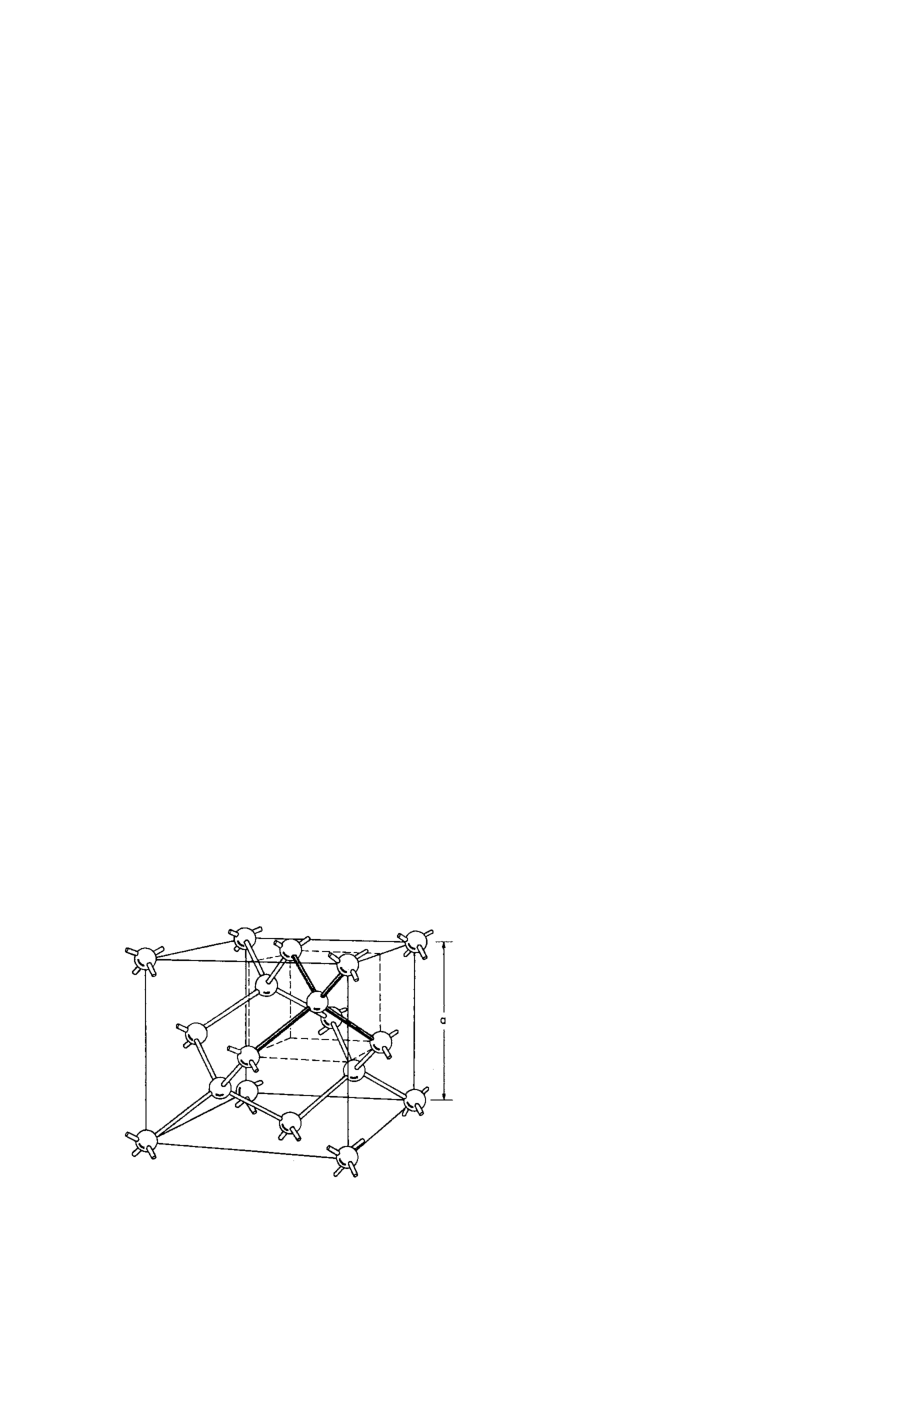
\includegraphics{diamondLattice.pdf} % requires the graphicx package
   \caption{\label{fig:diamondLattice}Diamond (a) and zinc blend (b) lattice. (After~\cite{Lutz:411172})}
\end{figure}

Due to the Pauli exclusion principle, electrons in crystals are organised in energy bands, 
each one containing many closely spaced levels; Figure~\ref{fig:EnergyLevels} helps in picturing 
the situation for diamond lattice. At very large distances each atom has the same two energy levels; 
the energy levels are $N$-fold degenerate ($N$ being the number of atoms), they indeed split 
into $N$ closely spaced levels when the atoms are brought close together. 
For $N\to\infty$, one speaks of energy bands, rather than levels, and these bands broaden, merge 
and split again with even closer spacing~\cite{Lutz:411172}.

\begin{figure}[htbp]
   \centering
   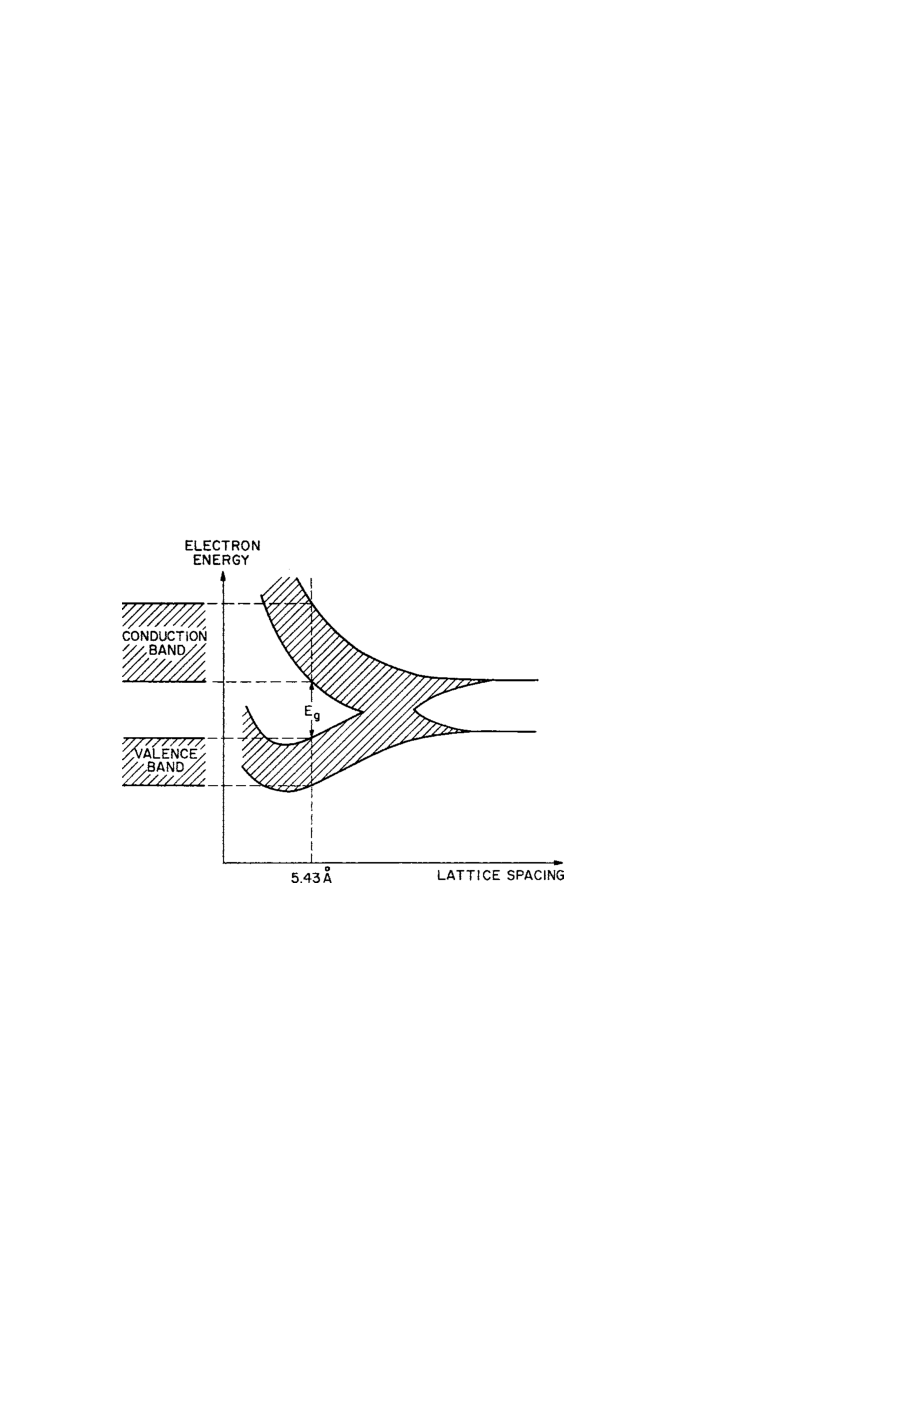
\includegraphics{EnergyLevels.pdf} % requires the graphicx package
   \caption{\label{fig:EnergyLevels}Energy levels of silicon atoms arranged in a diamond structure, as a function of lattice spacing. (After~\cite{Lutz:411172})}
\end{figure}

The spacing corresponding to silicon is indicated in Figure~\ref{fig:EnergyLevels} and corresponds to 
the minimum total energy of the electrons and the lattice, not very far from the minimum energy of
 the electrons in the filled valence band. 
 At low temperature one has a completely filled valence band and an empty conduction band; at room 
 temperature the thermal energy is high enough to lift a few electrons to the conduction band, thus 
 creating a weak conductivity due to free electrons and electrons vacancies, {\it i.e.} holes.
In Figure~\ref{fig:EnergyBandGap} the energy band structures of several materials are reported, 
including semiconductors.

 
 \begin{figure}[htbp]
   \centering
   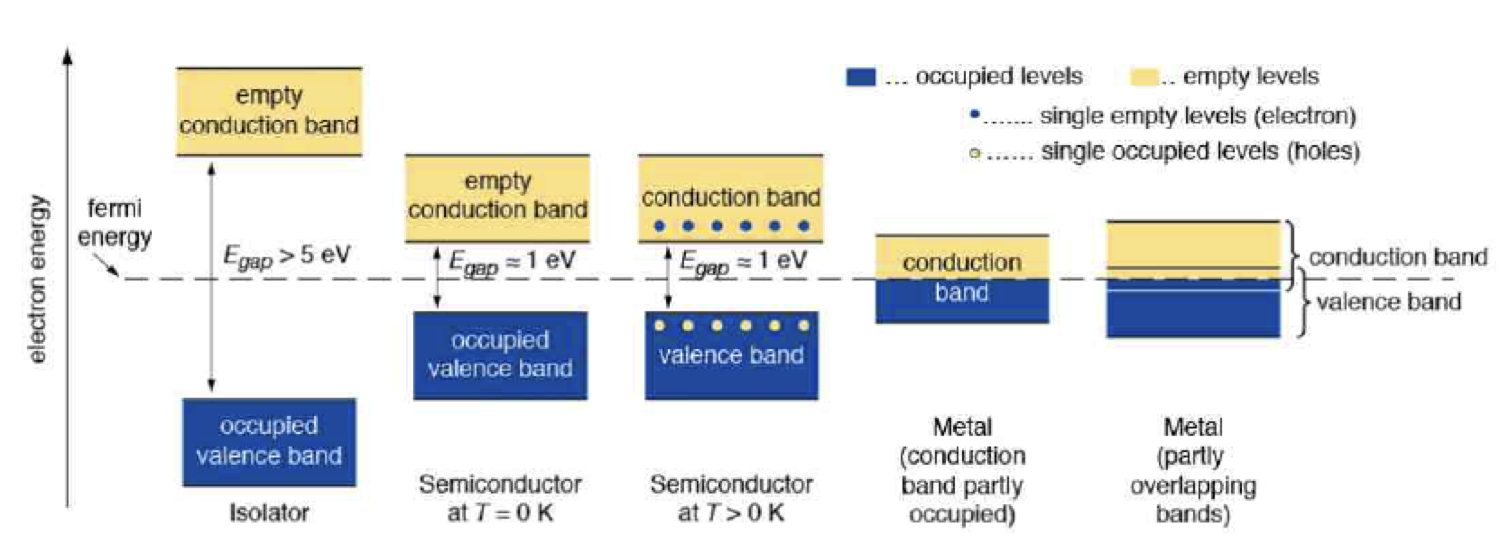
\includegraphics[width=0.8\textwidth]{EnergyBandGap.png} % requires the graphicx package
   \caption{\label{fig:EnergyBandGap}Energy band structure of several materials. For 
   semiconductors the  $T=0$~K and $T>0$~K situations are reported; for metals two 
   possible band configurations are represented (After~\cite{Krammer}).}
\end{figure}


 The structure of an isolator, or insulator, is similar to that of a semiconductor,  except that the band gap is much larger so that 
 the occupation probability of states in the conduction band is zero.   Conductors may either have 
 overlapping valence and conduction bands  or a partially filled conduction band. 
 We can conclude that the main difference between conductors, semiconductors and insulators 
 is the value of the band gap energy $E_g$.
 
 \begin{figure}[htbp]
   \centering
   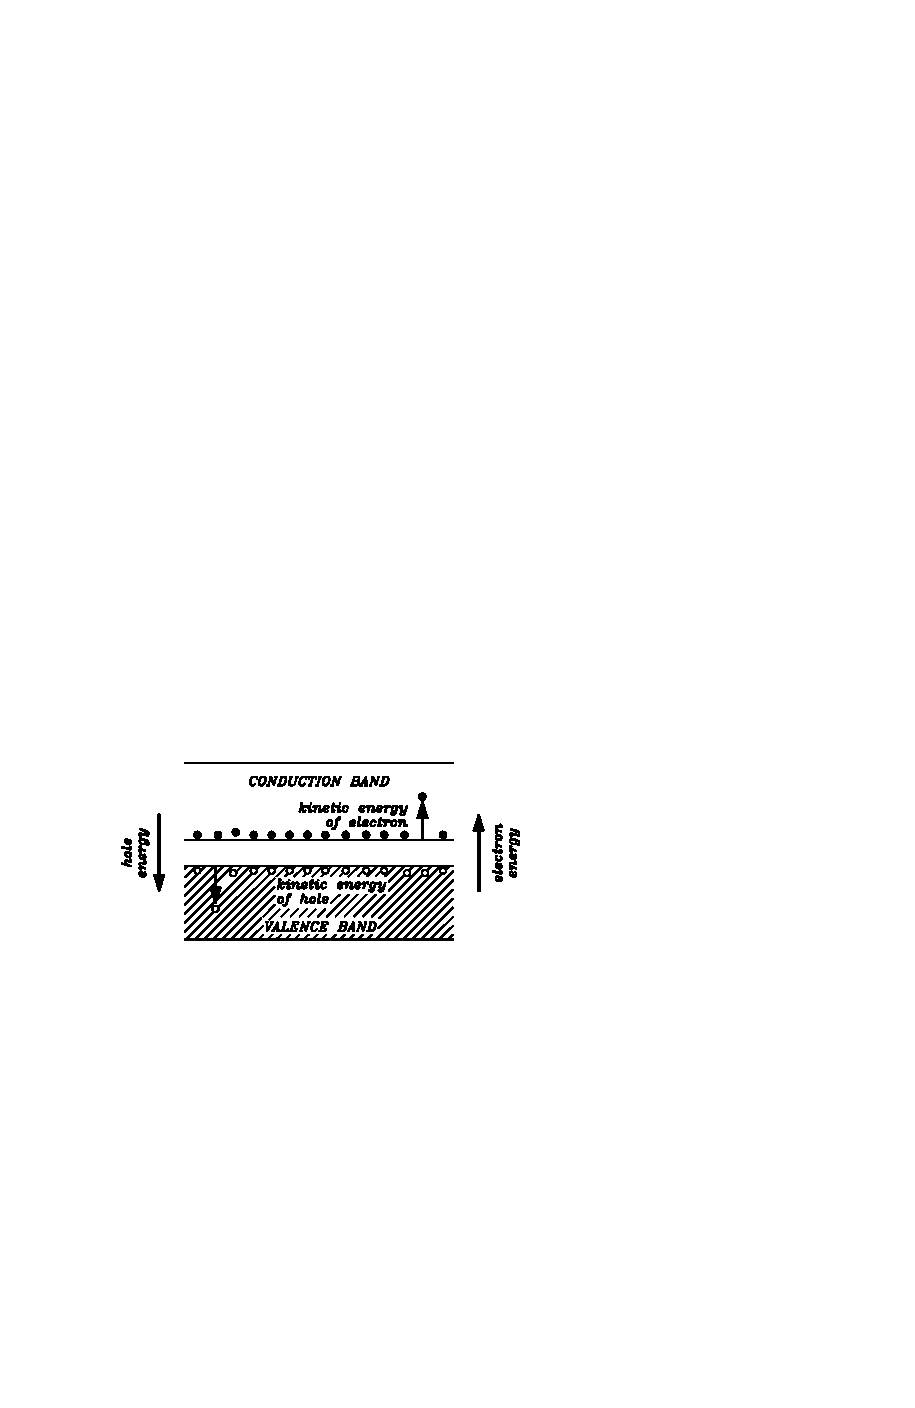
\includegraphics[width=0.55\textwidth]{KinEnergy.pdf} % requires the graphicx package
   \caption{\label{fig:KinEnergy}Potential and kinetic energy in the band 
   representation (After~\cite{Lutz:411172}).}
\end{figure}

Focusing on the dynamics of carriers in crystalline materials, it can be proven that  electrons in the 
conduction band and holes in the valence band are similar to free particles  but with an effective 
mass 
($m_n^*$, $m_p^*$) different from elementary electrons not imbedded in the lattice.
This mass is furthermore dependent on other parameters such as the direction of movement with 
respect to the crystal axis. The kinetic energy of electrons is measured from the lower edge of the 
conduction band upwards, that of the holes downward from the upper edge of the valence band; 
Figure~\ref{fig:KinEnergy} presents the energy diagram for free electrons and holes in lattice.

This simplified picture presents important limitations; in particular it neglects the relative position 
in lattice reciprocal space of the minimum conduction band and the maximum of the valence band. 
If there is no difference among the two positions then the semiconductor is said to have ``direct'' 
bandgap; otherwise it is an indirect semiconductor. Figure~\ref{fig:bandStructures} shows the difference 
between indirect semiconductors, like Silicon and Germanium, and direct ones, like Gallium Arsenide. 


 \begin{figure}[htbp]
   \centering
   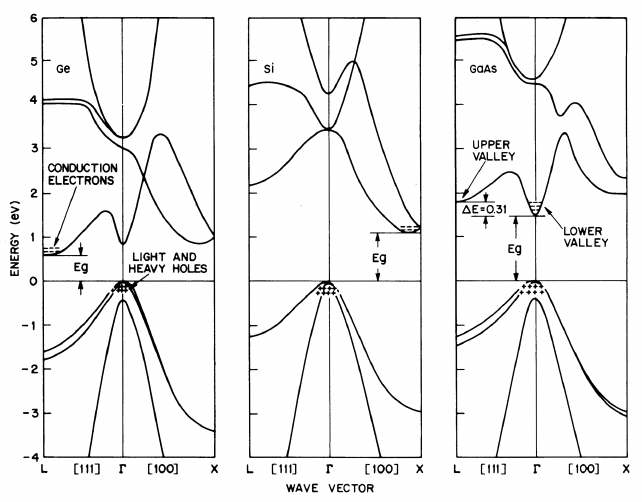
\includegraphics[width=0.55\textwidth]{bandStructures.jpg} % requires the graphicx package
   \caption{\label{fig:bandStructures}Germanium (left), Silicon (center) and Gallium Arsenide (right) band structures. (Bottom) valence bands; (top) conductive bands.}
\end{figure}

For indirect semiconductors, the process of creation or annihilation of an electron-hole pair requires 
not only a quantum of energy, like a photon, but also a net lattice momentum transfer, thanks to 
phonons. In Silicon at room temperature the bandgap energy value is of about $E_g\sim1.12$~eV, 
while the mean ionisation energy $\epsilon$ is $\sim$~3.6~eV: the difference is due to the distance in the 
lattice reciprocal space of the edge of the conductive and the valence band. 

\subsection{Extrinsic Semiconductors and Doping}

Intrinsic semiconductors contain a very limited number of impurities  compared with the number of 
thermally generated electrons and holes. 
Electron states with energy $E$ are occupied following the Fermi-Dirac statistics:
\begin{equation}
F(E)=\dfrac{1}{1+\exp{\Bigg(\dfrac{E-E_F}{kT}}\Bigg)}
\label{eq:FermiDirac}	
\end{equation}
where $E_F$, the Fermi energy, is the energy at which the occupation probability of a (possible) 
state is one half, $k$ is the Boltzmann constant and $T$ is the absolute temperature. 
In Intrinsic semiconductors electrons and holes exist on account of thermal creation of electron-hole 
pairs, so we have:

\begin{equation}
p=n,
\label{eq:n=p}
\end{equation}
{\it i.e.} the concentration of electrons $n$ equals that of holes $p$. 
We will assert the mass action law for semiconductors:
\begin{equation}
np=n_i^2
\label{eq:massLawAction}
\end{equation} 
where $n_i$ is the {\it intrinsic carrier concentration}. The intrinsic carrier concentration depends only 
on the temperature $T$, the effective mass of the carriers $m^*$ 
and the band gap energy 
$E_g$~\cite{Lutz:411172}.


Intrinsic semiconductors are rarely used in semiconductor 
devices since it is extremely difficult to obtain sufficient purity in the material. Moreover, in most cases 
one intentionally alters the property of the material by adding small fractions of specific impurities. 
This procedure is called {\it doping}. 
 Doping is the replacement of a small number of atoms in the lattice by 
atoms of neighbouring columns from the atomic table (with one valence electron more or less compared 
to the basic material). Depending on the type of added material, one obtains $n-$type 
semiconductors with an excess of electrons in the conduction band or $p-$types with additional holes in 
the valence band. 

Doping Silicon with an element of the V group (P, As, Sb) leaves a valence electron of dopant atom 
loosely bound; those atoms are identified  
as {\it donor} dopants. The energy level of the donor is just below the edge of the conduction band; 
at room temperature most electrons are raised from the donor dopant to the conduction band.  
The doping with donors  is illustrated in Figure~\ref{fig:nDoping}. A semiconductor doped with 
donors is called a $n-$type semiconductor. There is an imbalance between 
electrons over holes in $n$-type semiconductors; electrons are the majority carriers, while holes the
minority ones. 

 \begin{figure}[htbp]
   \centering
   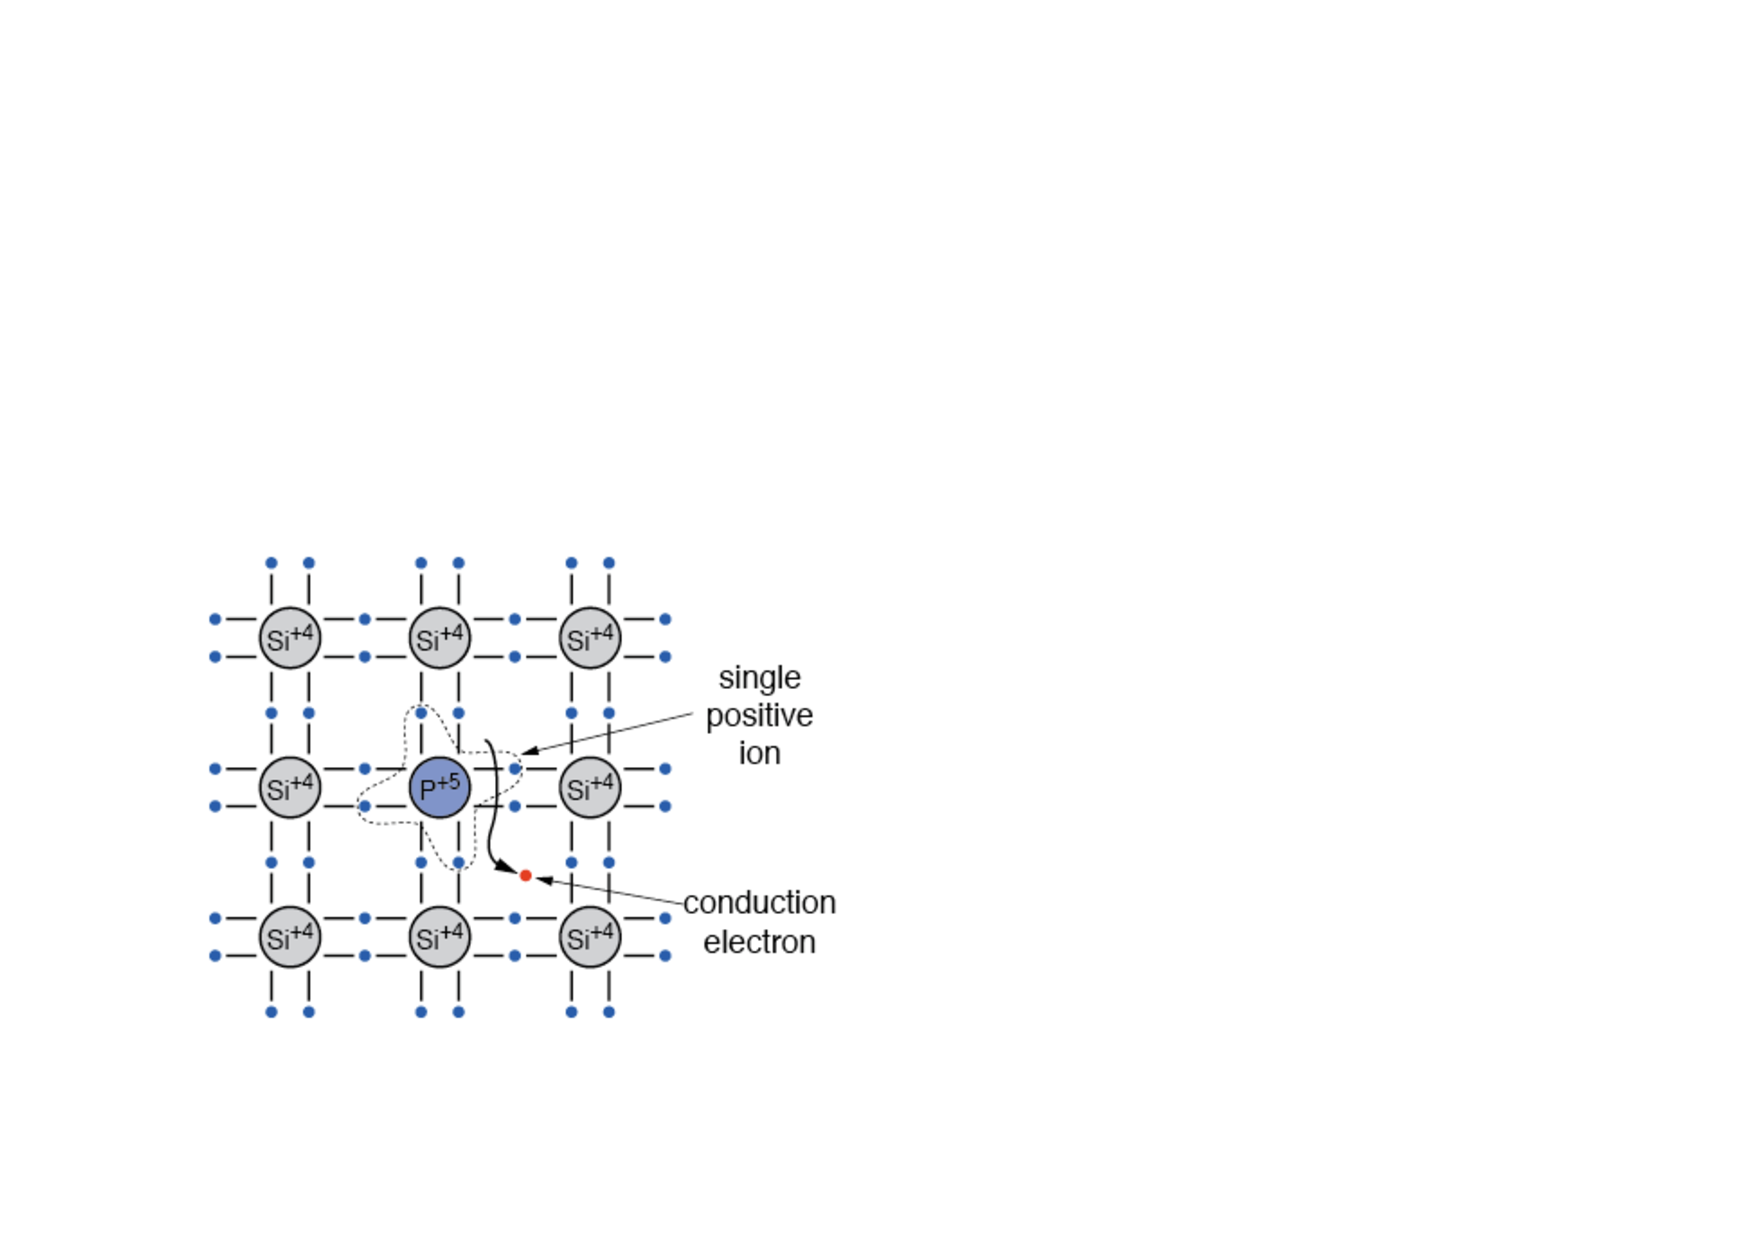
\includegraphics[width=0.45\textwidth]{nDopingBonds.pdf} 
   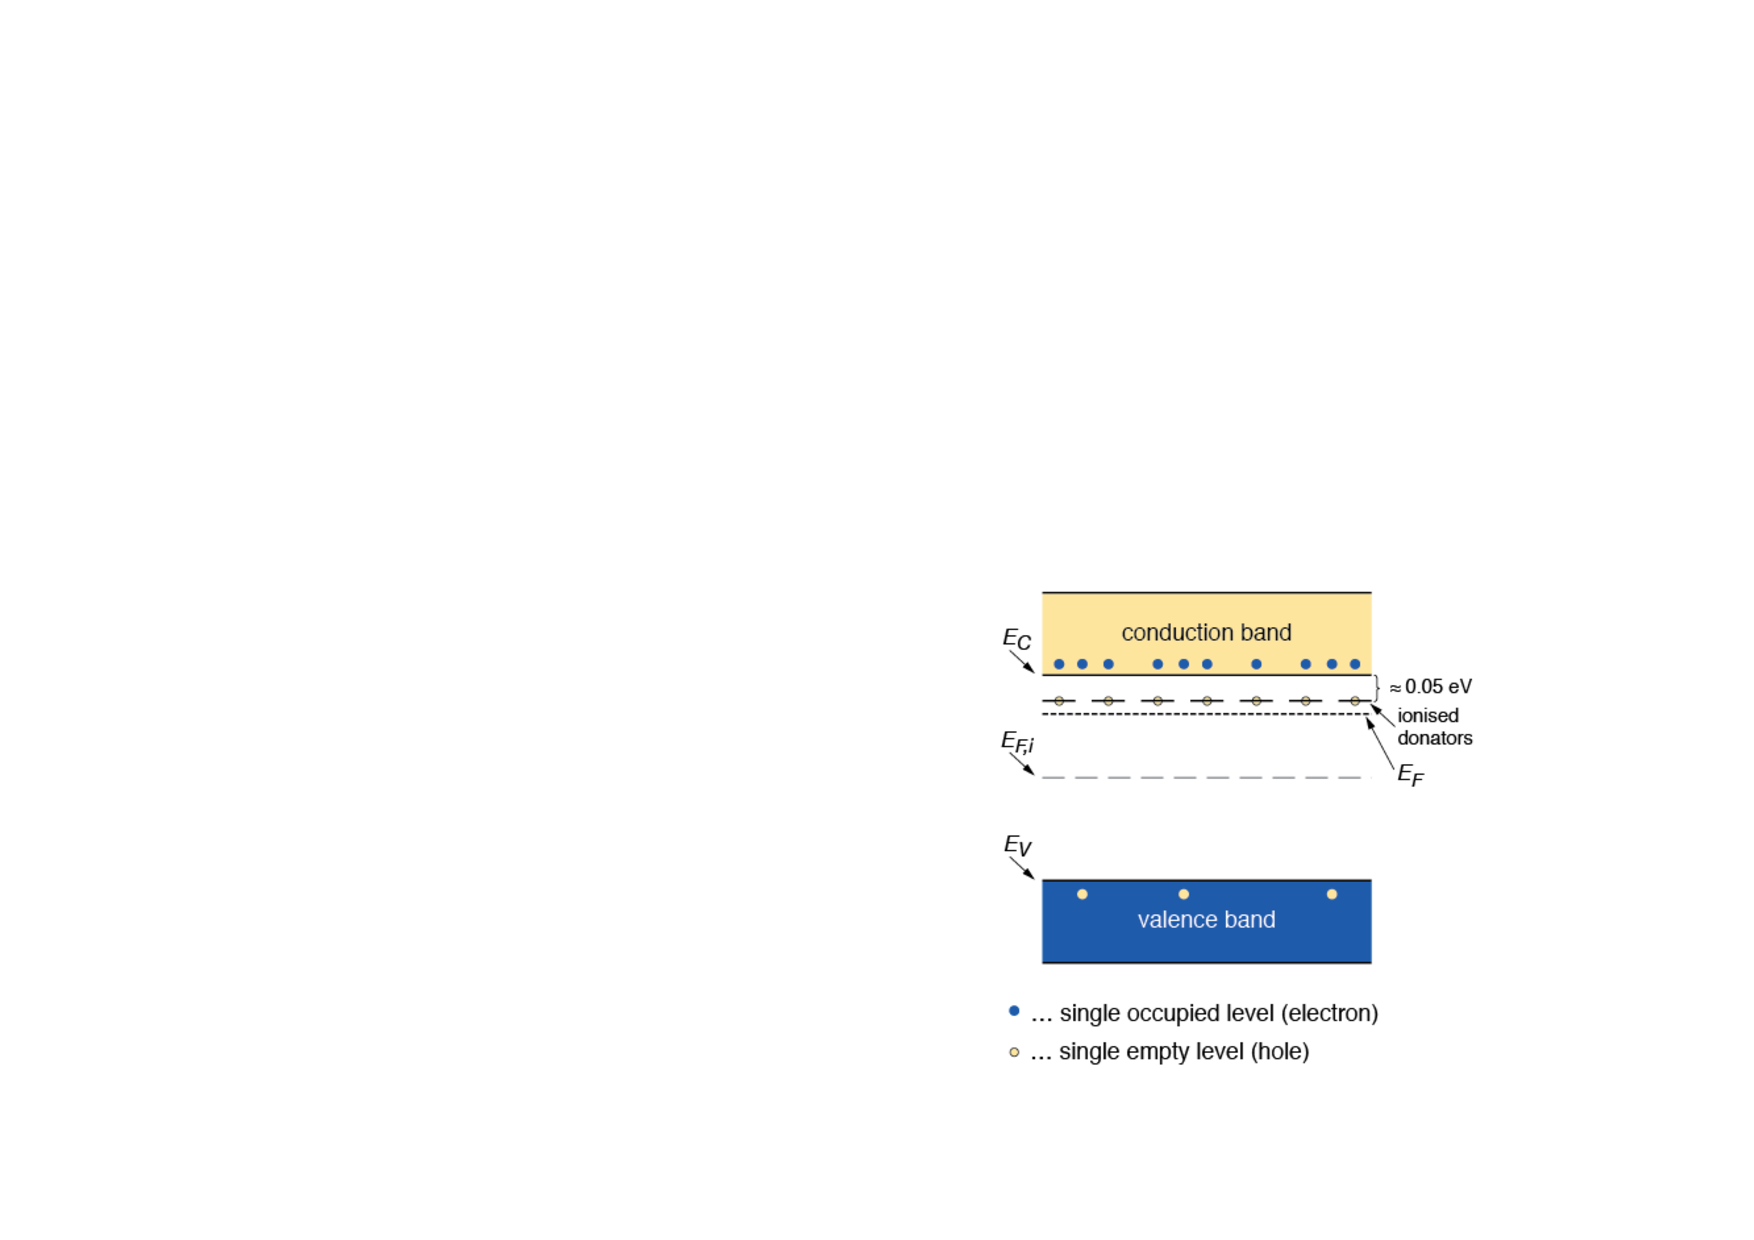
\includegraphics[width=0.35\textwidth]{nDopingBands.pdf} 
   \caption{\label{fig:nDoping}Doping Silicon with donor atoms. (Left) atom bonds with donor dopant; 
   (right) energy bands diagram after donor doping. (After~\cite{Krammer})}
\end{figure}

Doping Silicon with an element of the III group (B, Al, Ga, In) leaves one valence bond open; 
those atoms are identified  as {\it acceptor} dopants. 
The energy level of the acceptor is just above the edge of the valence band; 
at room temperature most levels are occupied by electrons leaving holes in the valence band.  
The doping with acceptors  is illustrated in Figure~\ref{fig:pDoping}. A semiconductor doped with 
acceptors is called a $p-$type semiconductor. There is an imbalance between 
holes over electrons in $p$-type semiconductors; holes are the majority carriers, while electrons the
minority ones.



 \begin{figure}[htbp]
   \centering
   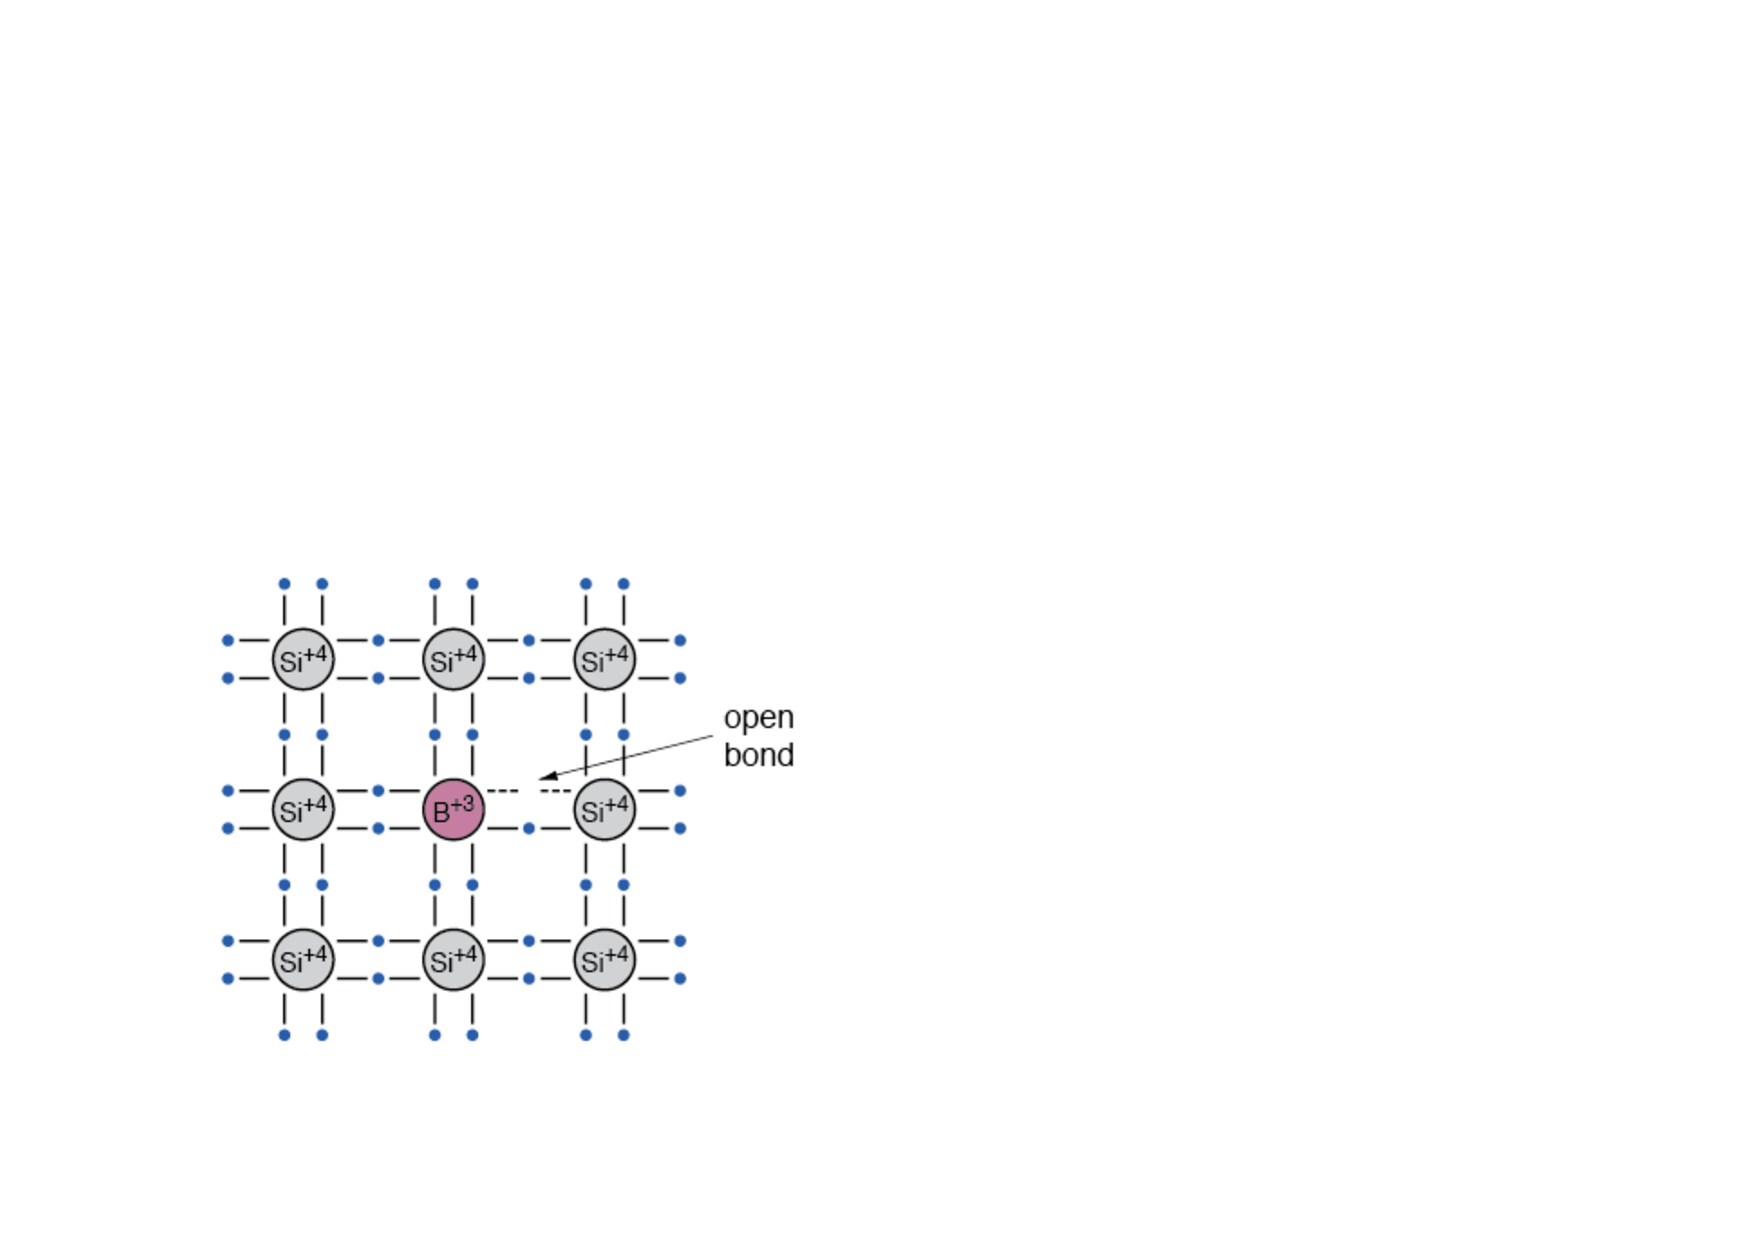
\includegraphics[width=0.45\textwidth]{pDopingBonds.pdf} 
   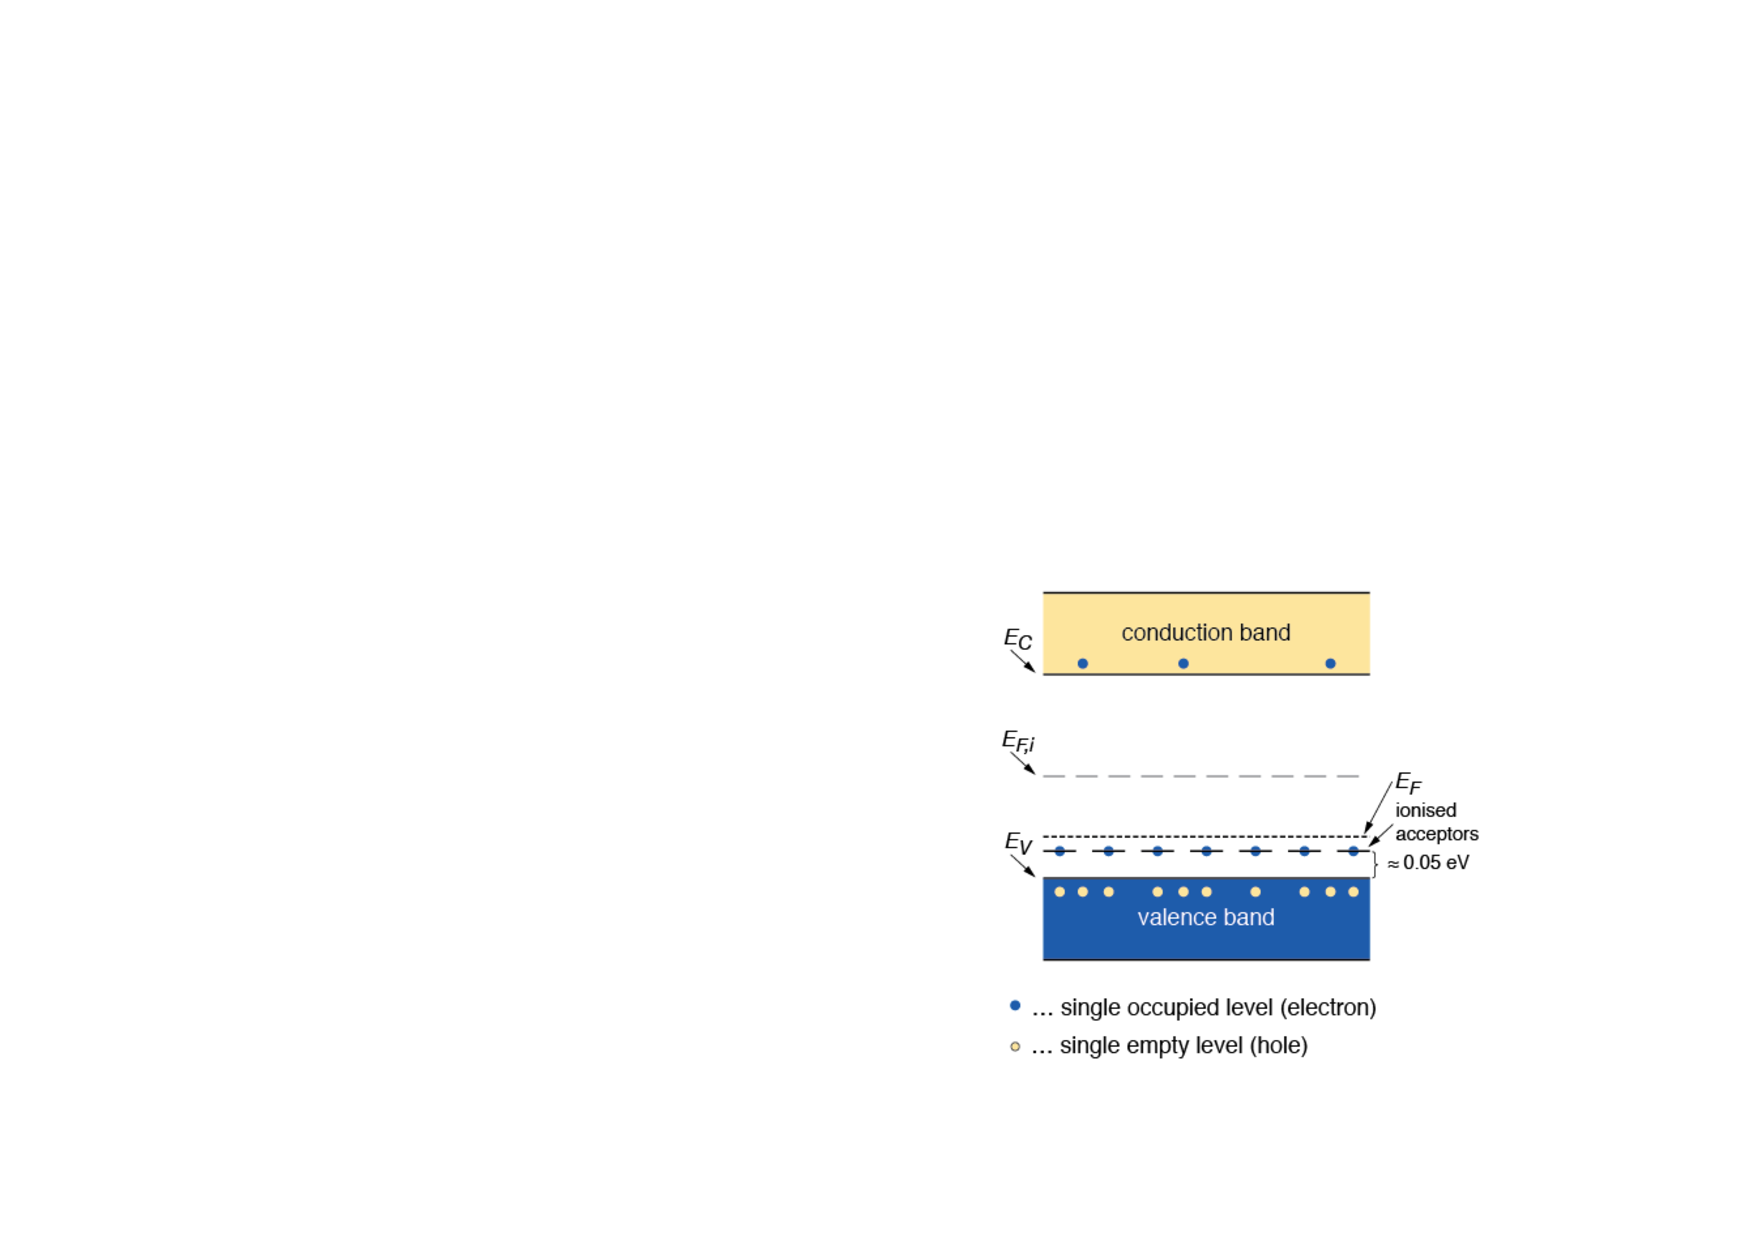
\includegraphics[width=0.35\textwidth]{pDopingBands.pdf} 
   \caption{\label{fig:pDoping}Doping Silicon with acceptor atoms. (Left) atom bonds with acceptor 
   dopant; (right) energy bands diagram after acceptor doping.(After~\cite{Krammer})}
\end{figure}
In a doped semiconductor the relation $n=p$ does not hold, while the mass action law  
(Eqution~\ref{eq:massLawAction}) still does. Semiconductors where $n\neq p$ are called
 {\it extrinsic}.
In a doped semiconductor electrons are merely redistributed among the various energy states, 
but not taken out of or put into the semiconductor itself, the crystal remains electrically neutral. 
The equation that states this charge-neutrality condition reads:

\begin{equation}
n+N_a^-=p+N_d^+,
\label{eq:chargeNeutrality}
\end{equation}

where $N_{a(d)}^{-(+)}$ represent the charge density of ionised acceptors (donors) respectively. 
At room temperature dopants are normally ionised so it is safe to assume that $N_a^-\simeq N_a$ 
and $N_d^+\simeq N_d$, hence $n-p=N_d-N_a$. From charge neutrality and mass action law  
it can be easily shown that for an $n$-type semiconductor the concentration of electrons $n$ is 
equal to that of the donor dopants $N_d$ to a very good level; with the same reasoning in a 
$p$-type semiconductor the concentration of holes $p$ is equal to that of the acceptor 
dopants $N_a$. 

The Fermi level for the intrinsic semiconductor $E_i$ lies very close to the middle of the bandgap.
 When 
impurity atoms are introduced, the Fermi level must adjust itself to preserve charge neutrality. 
We assert that the in an $n$-type semiconductor where the donors concentration is $N_d$ the 
Fermi level at temperature $T$ is:

\begin{equation}
E_F=E_C-kT\ln\Big(\dfrac{N_c}{N_d}\Big)
\label{eq:nEF}
\end{equation}
where $N_c$ is the effective density of states in the conduction band. 
Similarly, in a $p$-type semiconductor where the acceptors concentration is $N_a$ the 
Fermi level at temperature $T$ is:

\begin{equation}
E_F=E_V+kT\ln\Big(\dfrac{N_v}{N_a}\Big)
\label{eq:pEF}
\end{equation}
where $N_v$ is the effective density of states in the valence band. 

The Equations~\ref{eq:nEF}~and~\ref{eq:pEF} can be expressed also as a function of the 
electrons and holes thermal equilibrium concentration $n,p$, and the intrinsic carrier concentration 
$n_i$, to evaluate  the distance of the Fermi level $E_F$ from the intrinsic value $E_i$ 
in an extrinsic semiconductor:

\begin{align}
E_F&=E_i+kT\ln\Big(\dfrac{n}{n_i}\Big)\label{eq:nEini}\\
E_F&=E_i-kT\ln\Big(\dfrac{p}{n_i}\Big)\label{eq:pEini}
\end{align} 




\subsection{Carrier Transport in Semiconductors and Continuity Equations}

So far only semiconductors in equilibrium have been considered. We will now deal with 
semiconductors out of equilibrium through the application of an external voltage or because 
hit by light. These conditions will lead to an inhomogeneous distribution of charge carriers that 
we will describe through the {\it continuity equations}. But before
 getting to the continuity equations let's 
review very briefly the mechanisms of transport of the 
carriers, the drift and the diffusion.

If an electric field is present the charge carriers will be accelerated in between random collisions  
with the lattice 
(the typical time between collisions $\tau_c$ is of about 10$^{-12}$~s), 
in a direction determined by the electric field and a net average drift velocity will be obtained, 
equal to:
\begin{align}
\vec{v}_n=-\dfrac{q\tau_c}{m_n}\vec{E}&=-\mu_n\vec{E}\label{eq:nDrift}\\
\vec{v}_p=\dfrac{q\tau_c}{m_p}\vec{E}&=\mu_p\vec{E}\label{eq:pDrift}
\end{align}
where $\vec{v}_n$ and $\vec{v}_p$ are the drift velocities.
The parameters $\mu_n,\mu_p$ are the electrons and holes mobilities, respectively. 
For fields small enough the mobilities are constant, while at large fields the carrier velocities 
reach their saturation values $v_{s,n}$ and $v_{s,p}$. Other than on the electric field mobilities depend on 
temperature, and doping levels too.

If we now consider an inhomogeneous distribution of free charge carriers in a semiconductor crystal 
and neglect all effects that are due to electric fields it can be shown that there is a net flow 
of charges that smooths the charge distribution. This effect is called diffusion and it is mathematically 
described by the diffusion equation:
\begin{align}
\vec{F}_n=-D_n\nabla{n}\label{eq:nDiff}\\
\vec{F}_p=-D_p\nabla{p}\label{eq:pDiff}
\end{align}
Here $\vec{F}_{n,p}$ are the fluxes, $D_{n,p}$ the diffusion constants and 
 $n,p$ the carrier concentrations,  of electrons and holes respectively.

Combining the effects of drift and diffusion, one obtains the current densities:
\begin{align}
\vec{J}_n=q\mu_nn\vec{E}+qD_n\nabla{n}\label{eq:nCurrf}\\
\vec{J}_p=q\mu_pp\vec{E}-qD_p\nabla{p}\label{eq:pCurr}
\end{align}
$q$ is the absolute value of the charge of the electron.

Mobility and diffusion are related to each other by the Einstein equation:

\begin{align}
D_n=\dfrac{kT}{q}\mu_n\label{nEinst}\\
D_p=\dfrac{kT}{q}\mu_p\label{pEinst}
\end{align}

In a semiconductor, electrons and holes are constantly generated by thermal excitation of electrons 
form the valence band to the conduction band. We call $G$ the  generation rate per unit of 
volume and $R$ the  recombination rate per unit of volume. 
The generation process is counterbalanced, under 
thermal equilibrium, by a recombination process in which electrons and holes annihilate each other. 
When excess carriers are present the recombination process outweighs the generation one. 
There are two basic processes by which electrons and holes may recombine with each other. In the 
first process electrons from the conduction band make direct transition to vacant states in the valence 
band. In the second process electrons and holes recombine through intermediary states known as 
{\it recombination centers}. The recombination centers are usually impurities and lattice imperfections 
of some sort. 
We define the recombination lifetime $\tau_r$ the average time it takes for a minority carrier to 
recombine. 


Now we can write the continuity equations which will describe the change in carrier concentration 
as the result of the drift, diffusion, generation and recombination phenomena:

\begin{align}
\dfrac{\partial n}{\partial t}&=\dfrac{1}{q}\nabla\cdot\vec{J}_n+G_n-R_n\label{eq:nCont}\\
\dfrac{\partial p}{\partial t}&=\dfrac{-1}{q}\nabla\cdot\vec{J}_p+G_p-R_p\label{eq:pCont}
\end{align}

The electric field $\vec{E}$ is linked to the charge distribution $\rho$ by the Poisson's equation:

\begin{equation}
\nabla\cdot\vec{E}=\dfrac{\rho}{\epsilon_{sc}\epsilon_{0}},
\label{eq:Poisson}
\end{equation}
where $\epsilon_{sc}$ is the relative permittivity of the semiconductor.
%\showthe\font



If in addition of an electric field a magnetic field is present too 
the path followed by electrons and holes is (on average) no longer parallel 
to the electric field. The movement of electrons and holes in the simultaneous presence of an electric and magnetic field is shown diagramatically in Figure~\ref{fig:LorentzAngle} 
(in Silicon $\vec H\sim\vec B/\mu_0$, where $\mu_0$ is the vacuum permeability).
\begin{figure}[htbp]
   \centering
   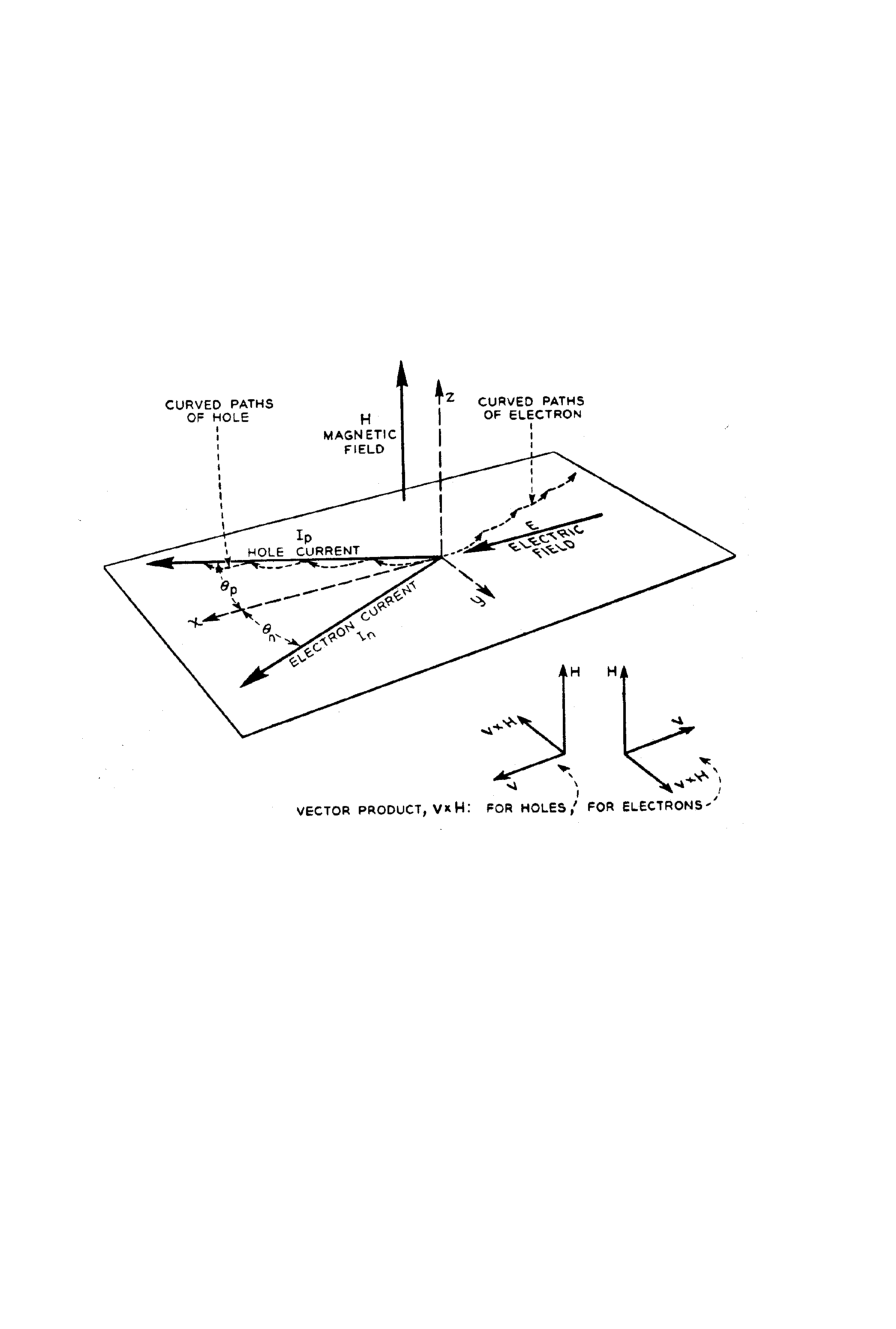
\includegraphics[width=0.55\textwidth]{LorentzAngle.pdf} 
   \caption{\label{fig:LorentzAngle}Electron and hole current in relation to electric and magnetic field. 
   (After~\cite{Shockley}).}
\end{figure}
The angular deviation $\theta_{n,p}$ from the electric field direction is called ``Lorentz angle''; its value 
is related to the 
magnitude of the magnetic field $B$ and the Hall mobilities $\mu_{n,p}^H$\footnote{they differ from 
the drift mobilities}:

\begin{equation}
\tan{\theta_{n,p}}=\mu_{n,p}^HB
\label{eq:LorentzAngle}
\end{equation}

\section{The p-n Junction}
\label{sec:pnjunction}

At the interface of an $n$-type and $p$-type semiconductor the difference in the Fermi levels cause 
diffusion 
of surplus carries to the other material until thermal equilibrium is reached. At this point the Fermi 
level 
is equal. The remaining ions create a 
space charge and an electric field stopping further diffusion. 
The stable space charge region is free of charge carries and is called the depletion zone. 
In Figure~\ref{fig:pnJunction} a p-n junction in thermal equilibrium, before and after its parts are 
brought in contact.

\begin{figure}[!htbp]
   \centering
   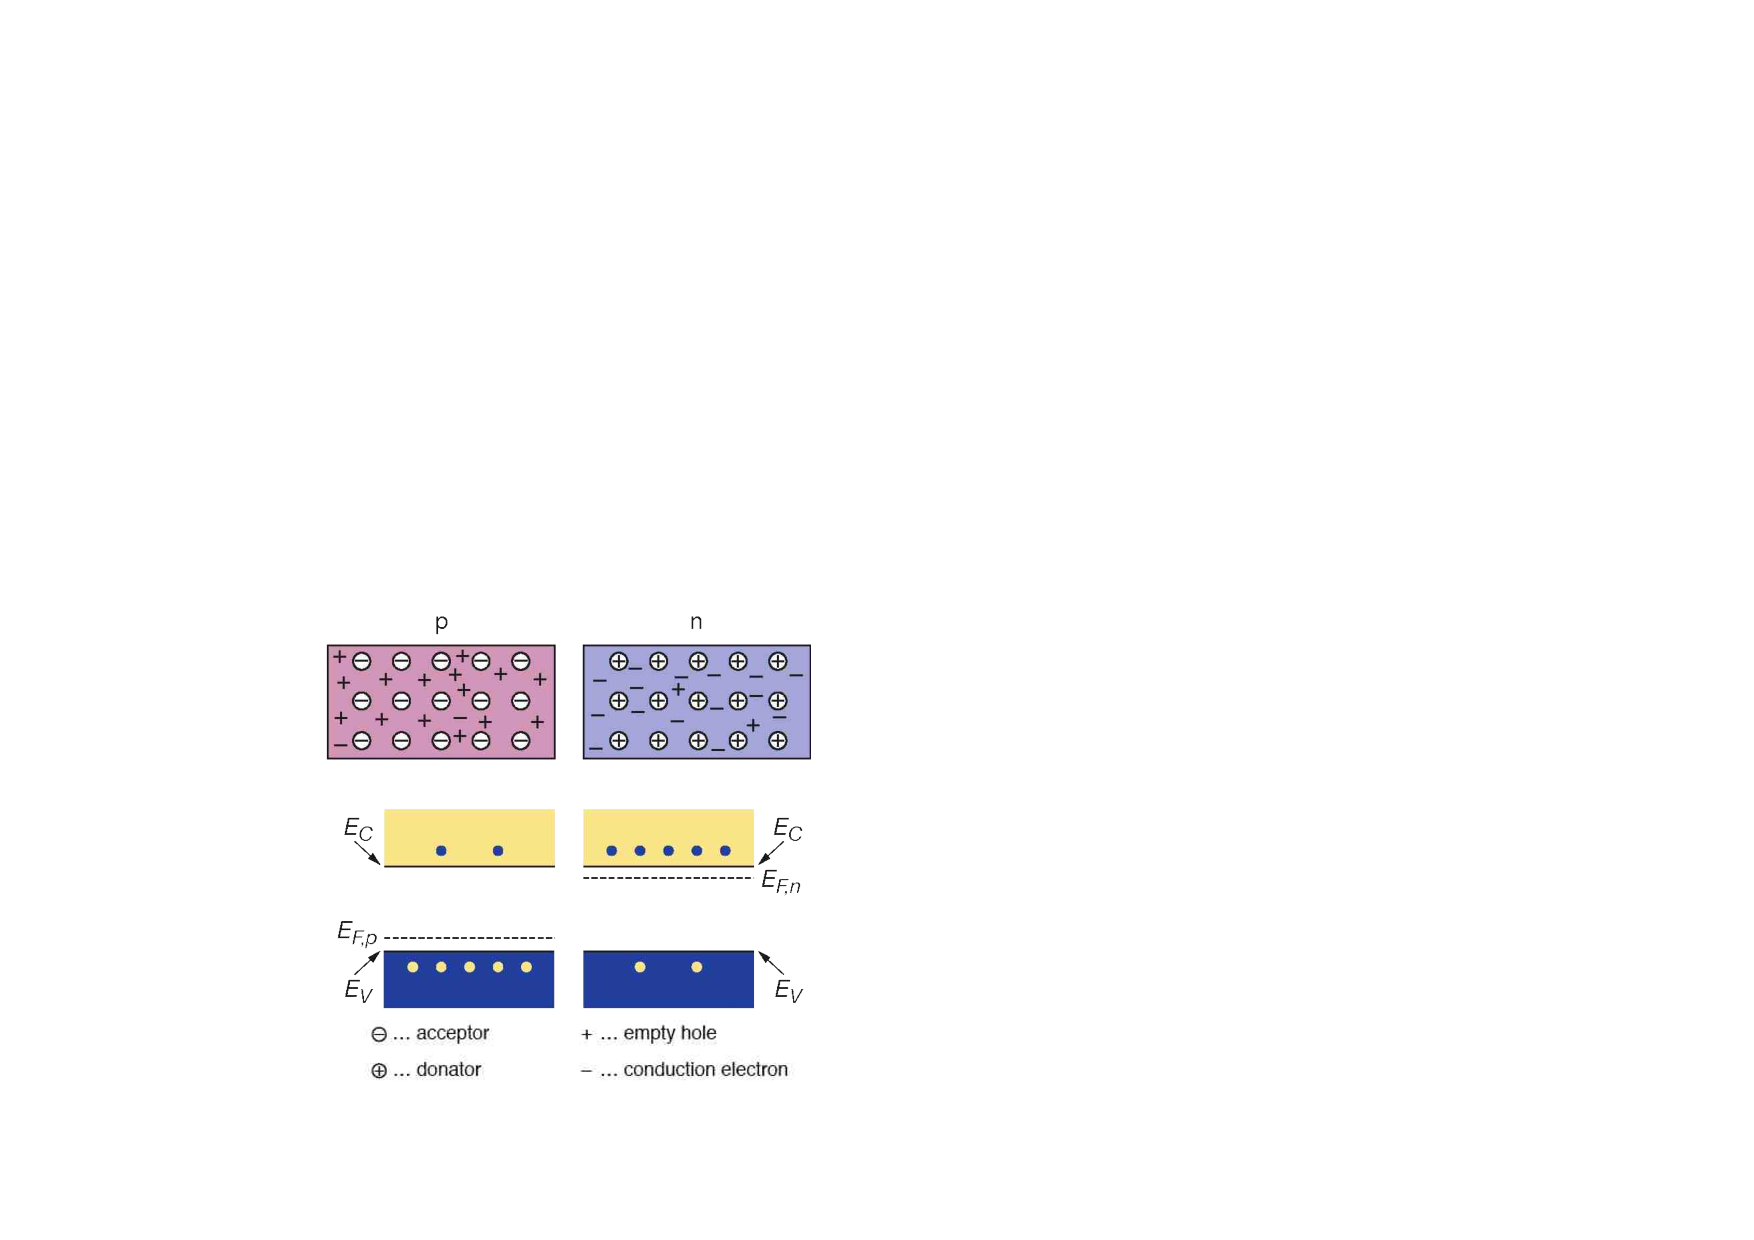
\includegraphics[width=0.45\textwidth]{p_close_to_n.pdf} 
   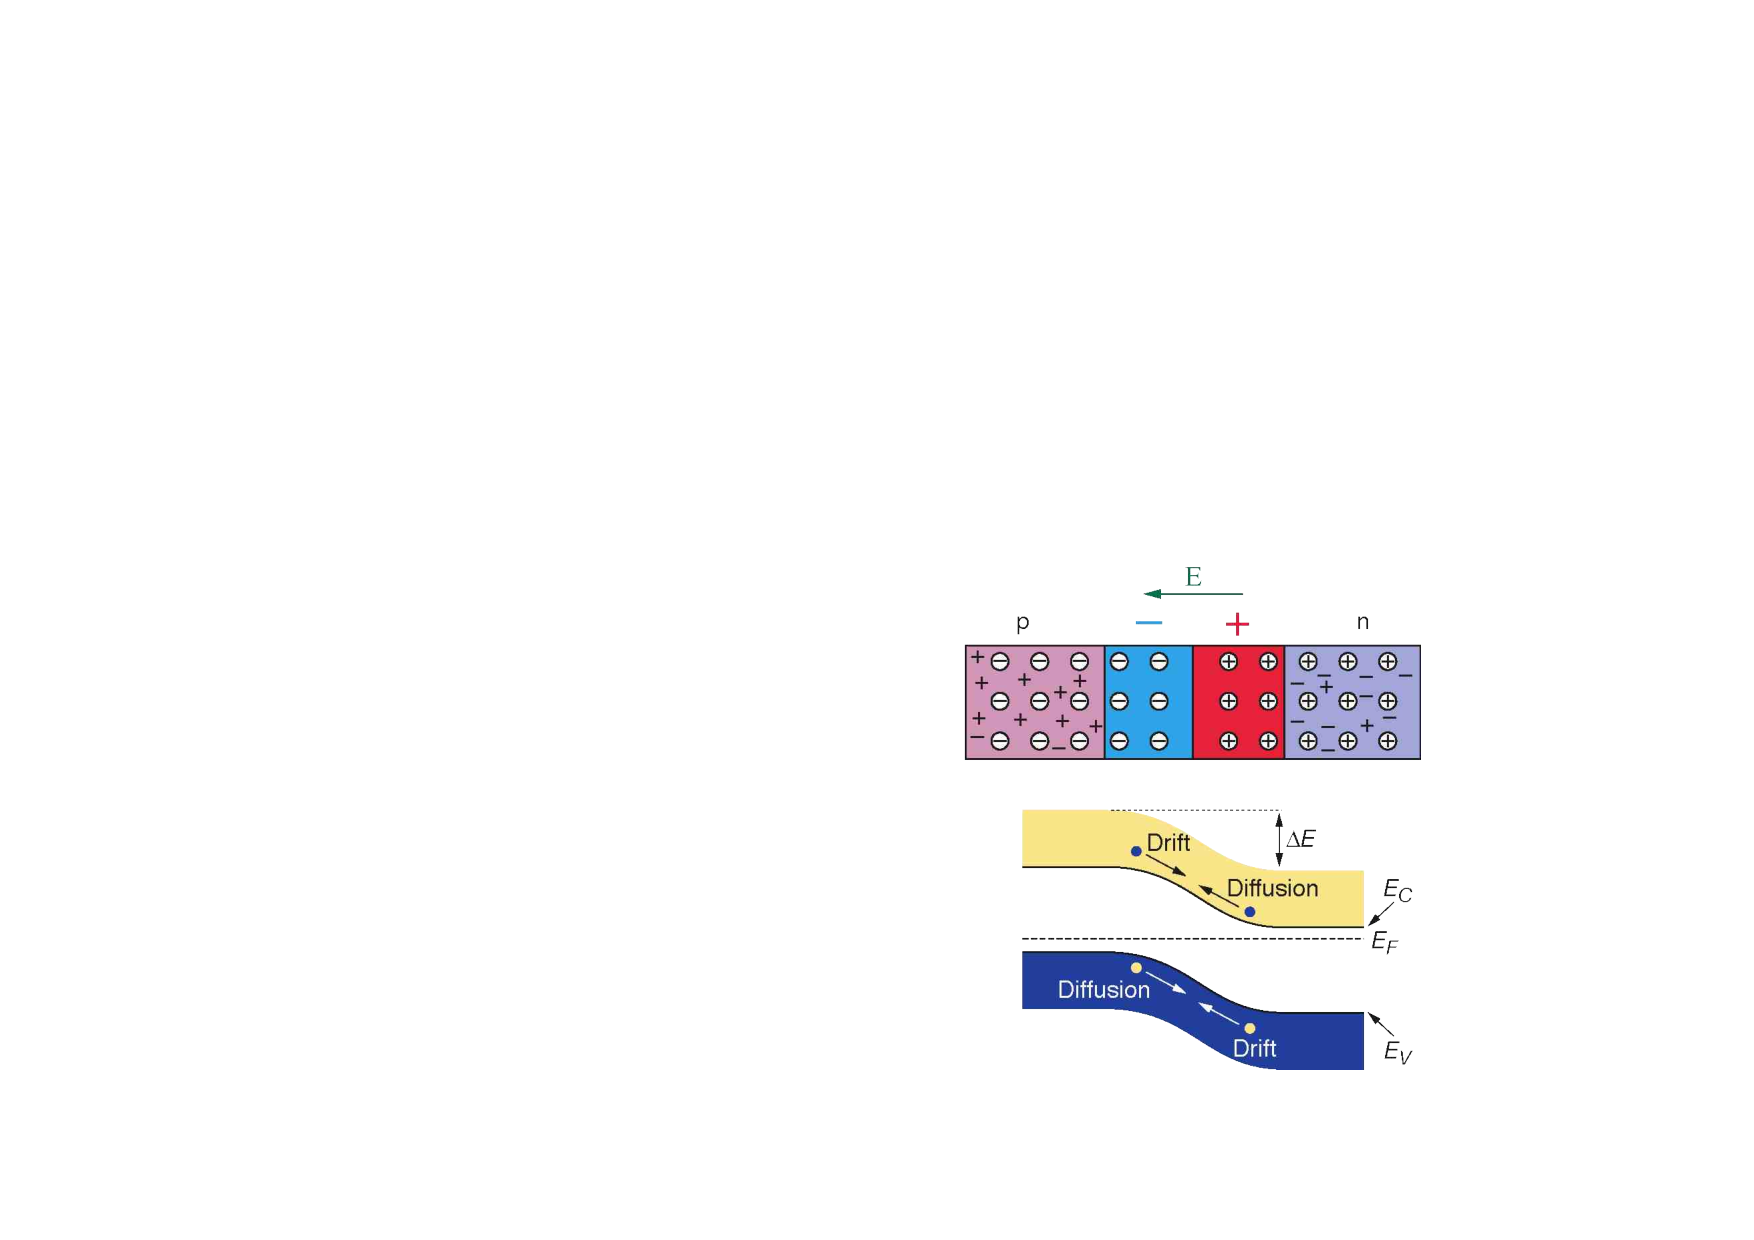
\includegraphics[width=0.45\textwidth]{pn_junction.pdf} 
   \caption{\label{fig:pnJunction}P-n junction formation. (Left) Two oppositely doped semiconductors 
   are compared. (Rigth) The p-n junction is formed. (After~\cite{Krammer}).}
\end{figure}



By applying an external voltage the depletion zone can be shrunk or enlarged. For particle detection 
purpose we are interested in maximising the depletion zone: within it there are virtually no 
free carriers and there is an electric field 
allowing the collection of the free carriers created by the ionising particles. 

By looking at Figure~\ref{fig:pnJunction} it is clear that to deplete more the junction volume 
a potential more positive on the $n$-side than on the $p$-side should be applied; we will refer 
to this polarisation as {\it reverse bias}~voltage.

In the following we will restrict ourselves to abrupt junctions, {\it i.e.} when the doping of both $p$- 
and $n$-type sides of the junction are uniform. Moreover we will consider only the case of 
asymmetric junctions, where one of the two sides is heavily doped, much more doped than the 
other one\footnote{The way in which these junctions are fabricated is beyond the scope of this 
report}. The heavily doped side is usually indicated with a $+$, hence we will talk of 
$p^+-n$ and $n^+-p$ junctions. In Figure~\ref{fig:AAJunction} the charge distribution of 
an abrupt asymmetric $n^+-p$ junction is depicted; the dopant concentration, the 
resulting bulk effective doping concentration and the bulk thickness are indicated too.

\begin{figure}[htbp]
   \centering
   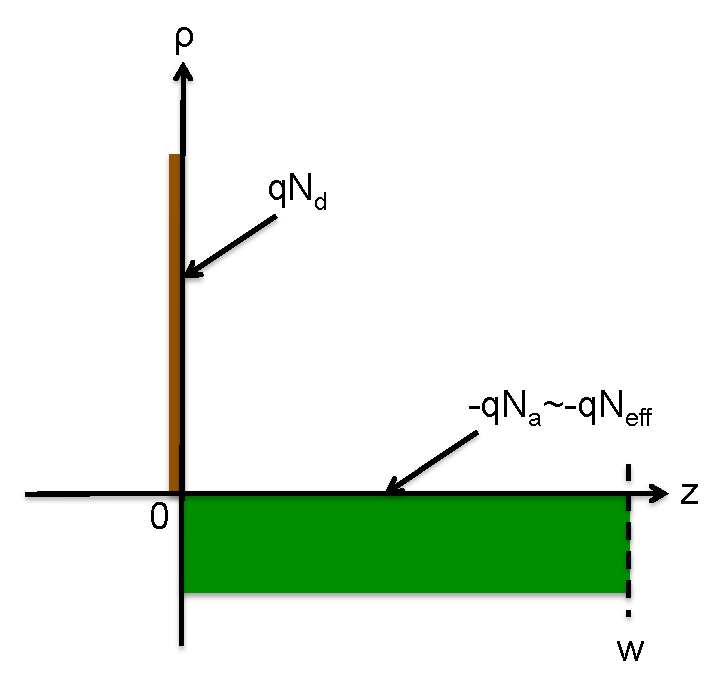
\includegraphics[width=0.45\textwidth]{Abrupt_Junction.pdf} 
      \caption{\label{fig:AAJunction}Charge distribution in an abrupt asymmetric $n^+-p$ junction.}
\end{figure}

To estimate the voltage needed to completely deplete the junction bulk we introduce the concept 
of {\it effective doping concentration} $N_{eff}$:

\begin{equation}
N_{eff} = N_d-N_a
\label{eq:Neff}
\end{equation}
which will reduce to simply $N_d$ for $p^+-n$ junctions and $-N_a$ for $n^+-p$ junctions.
By integrating twice the Poisson's equation over the semiconductor thickness we get 
the voltage needed to achieve the complete depletion of the 
junction volume, the so-called {\it depletion voltage} $V_{depl}$, whose absolute value is equal to:
\begin{equation}
V_{depl}=\dfrac{q|N_{eff}|w^2}{2\epsilon_{sc}\epsilon_0}
\label{eq:vdepl}
\end{equation} 
 where $w$ is the total thickness of the lightly doped semiconductor volume. We stress 
 the fact that the depletion voltage $V_{depl}$ depends linearly on the effective doping 
 concentration $N_{eff}$ and quadratically on the semiconductor volume $w$.

Particle detectors exploiting the $p-n$ junction properties are labelles according to the type 
of the bulk: $p$-type detectors feature a $p$-type bulk, the opposite goes for $n-$type detectors.

If the applied voltage is less than the depletion one we can evaluate the depletion extension 
$d_{depl}$
using again the Poisson's equation. It is instructive to express the result using the {\it resistivity} 
$\varrho$ of the doped semiconductor:

\begin{equation}
\varrho^{-1}=q(N_a\mu_p+N_d\mu_n)\simeq qN_{eff}\mu
\label{eq:resisitivity}
\end{equation}

In Equation~\ref{eq:resisitivity} first the most general expression is presented (under the assumption 
that the carriers concentrations are dominated by the dopants), then the approximated value for an 
abrupt and asymmetric junction is given; $\mu$ is the mobility of the majority carriers.
We can then express the depletion extension $d_{depl}$ as:

\begin{equation}
d_{depl} = \sqrt{2\epsilon_{sc}\epsilon_{0}\mu\varrho|V|}
\label{eq:depletion}
\end{equation}

Comparing Equations~\ref{eq:vdepl}~and~\ref{eq:depletion} a useful relation for under-depleted 
semiconductor bulks can be found:

\begin{equation}
d_{depl} = \sqrt{\dfrac{V}{V_{depl}}}w
\label{eq:dunderdepleted}
\end{equation}
where $V(<V_{depl})$ is the absolute value of the applied bias voltage.

In nowadays trackers for experiments at high energy colliders
 high resistivity materials are used ($\varrho\sim$
 serveral k$\Omega$cm); hence, for thicknesses $w$ of few hundreds of microns depletion voltages of 
 (far) less than 100~V are achieved.

In $p-n$ junctions under reverse bias an electric field is present; if we refer to the case represented 
in Figure~\ref{fig:AAJunction} the electric field distribution at depletion voltage along the bulk is like 
the one shown in Figure~\ref{fig:AAEField}.
\begin{figure}[!htbp]
   \centering
   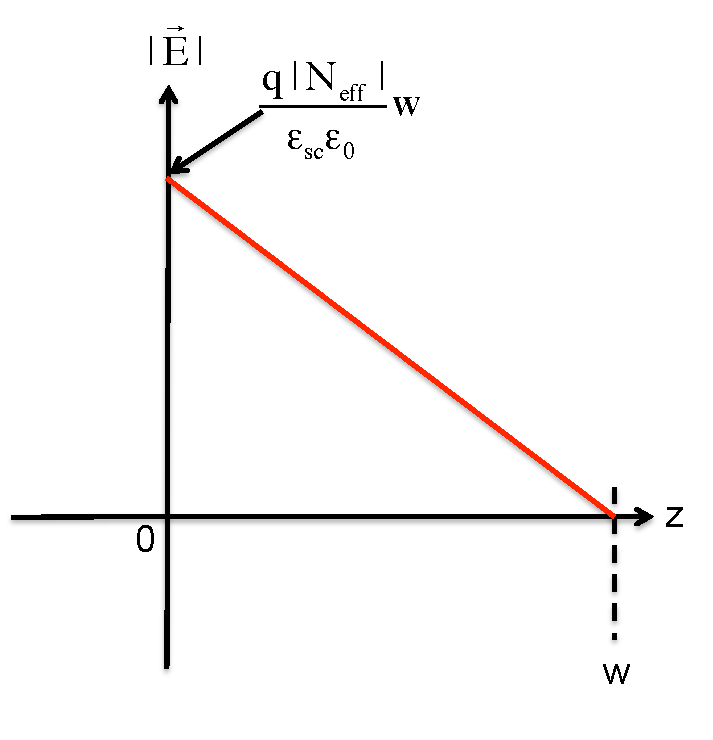
\includegraphics[width=0.45\textwidth]{E_Abrupt_Junction.pdf} 
    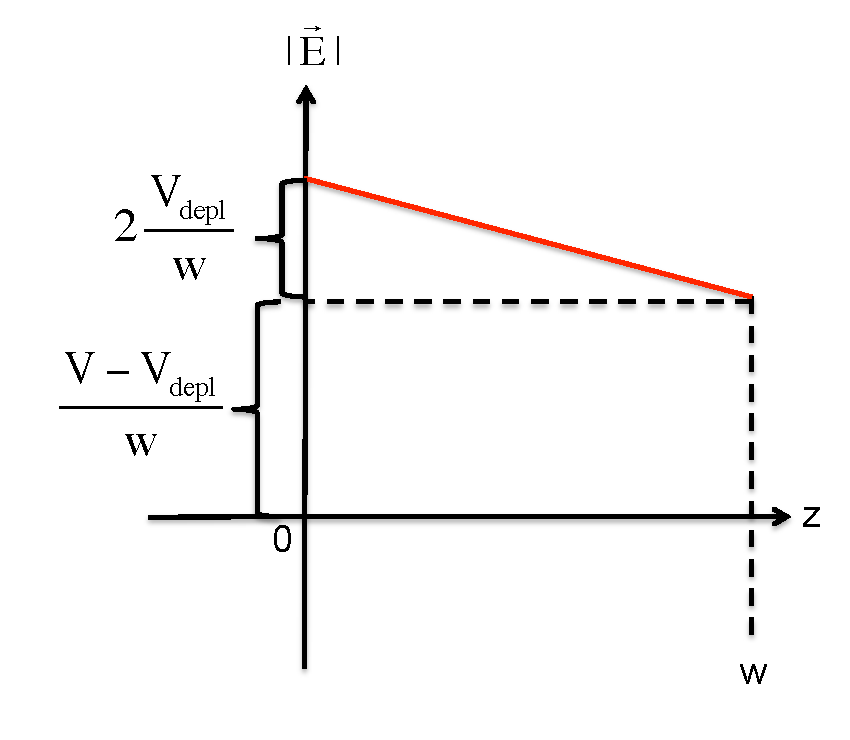
\includegraphics[width=0.45\textwidth]{Overdepleted_E_Abrupt_Junction.pdf}
   \caption{\label{fig:AAEField}Electric field profiles in an abrupt asymmetric $n^+-p$ junction.
   A doping profile like the one reported in Figure~\ref{fig:AAJunction} is assumed. 
   Electric field profile (left) at 
   depletion voltage; (right) in over depletion.}
\end{figure}
The electric field depends linearly on the bulk depth $z$, with a maximum at the 
junction; the maximum value is proportional to the effective doping concentration.

Still referring to Figure~\ref{fig:AAEField}, if a bias $V$ greater than the depletion 
voltage $V_{depl}$ is applied the electric field will 
have the following dependence on bulk depth $z$:

\begin{equation}
|\vec{E}(z)|=\dfrac{2V_{depl}}{w}\Big(1-\dfrac{z}{w}\Big)+\dfrac{V-V_{depl}}{w}
\label{eq:EFz}
\end{equation}
 The relation between the magnitude of the electric field and the position along the bulk is still 
 linear but now the electric field is non-zero everywhere. The bulk is said to be over-depleted.
 
 We have seen that the depleted region thickness $d_{depl}$ grows proportionally to the square root of 
 the applied (reverse) voltage $V$ (Eq.~\ref{eq:dunderdepleted}). A partially depleted 
 abrupt asymmetric junction can be modelled as  a parallel plate capacitor where 
 metallic plates are separated by $d_{depl}$. In the limit when $V<V_{depl}$
 it's then easy to derive the junction capacitance $C$:
 
 \begin{equation}
 C=\dfrac{A\epsilon_0\epsilon_{sc}}{w}\sqrt{\dfrac{V_{depl}}{V}}=A\sqrt{\dfrac{qN_{eff}\epsilon_0\epsilon_{sc}}{2}\dfrac{1}{V}}
 \label{eq:CV}
 \end{equation}
 where $A$ is the surface of the $p-n$ junction. Equation~\ref{eq:CV} is used to extract the 
 depletion voltage $V_{depl}$ and the effective doping concentration $N_{eff}$ in real 
 $p-n$ junctions. An example of a  $C^{-2}$ vs V plot for an $n-on-p$ diode is shown  in 
 Figure~\ref{fig:CV}. 
    
  
\begin{figure}[!htbp]
\centering
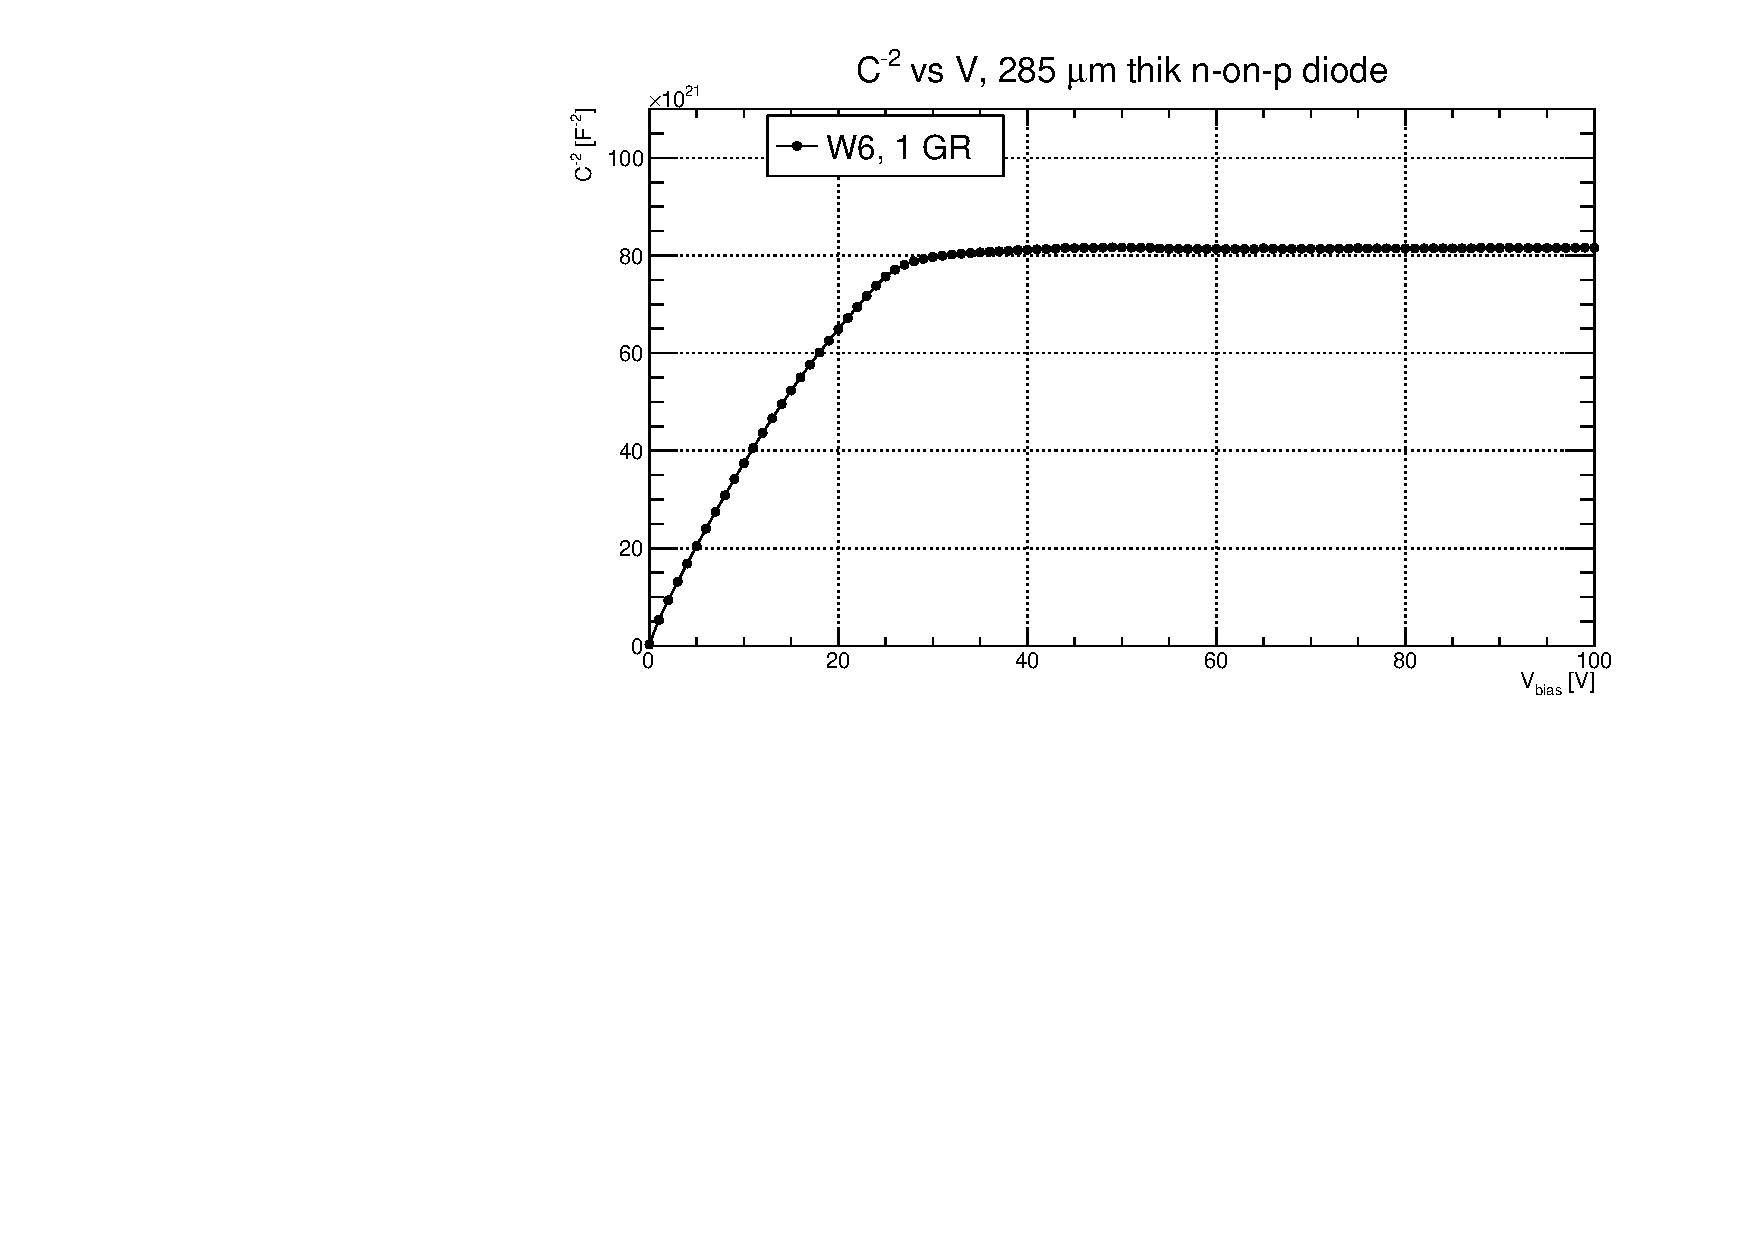
\includegraphics[width=0.5\textwidth]{C2V-n-in-p-291920-6-1GRs-GR1atGND-110704.pdf}
\caption{\label{fig:CV} $C^{-2}$~vs~V of a 285~$\mu$m thick $n-on-p$ diode.}
\end{figure}  
  
The bulk depletion corresponds to a linear increase of   $C^{-2}$, up to a ``kink'', after which the 
capacitance C is basically constant. The voltage at which the ``kink'' happens is a good estimate 
of the depletion voltage $V_{depl}$.
  
The depleted region of a $p-n$ junction is out of equilibrium; in particular, since $pn<n_i^2$, in the 
depleted region  the generation process is dominant over recombination. Thermally generated 
electron-hole paris are separated by the electric field and so they cannot recombine. A net 
flow of current appears, carriers will be collected at the ends of the semiconductor volume. 
If we assume a constant generation rate $G$ the generated current for a depleted semiconductor 
of area $A$ and thickness $w$ is equal to:

\begin{equation}
I_{leak}=\dfrac{qwA}{2}G
\label{eq:Ileak1}
\end{equation}
The subscript {\it leak} in Equation~\ref{eq:Ileak1}  stands for {\it leakage}: the current resulting 
from thermally generated carriers in the depleted region is dubbed as {\it leakage current}.

Equation~\ref{eq:Ileak1} can be rewritten introducing the concept of {\it generation lifetime} 
$\tau_g=n_i/G$:

\begin{equation}
I_{leak}=\dfrac{qn_iwA}{2\tau_g}
\label{eq:Ileak2}
\end{equation}
Nowadays Silicon material for ionising particle detectors can reach generation lifetimes  $\tau_g$
up to 1~s, for a current density $J$ of few pA/cm$^2$.

The leakage current of a depleted $p-n$ junction depends quite strongly on temperature: 
leakage current roughly doubles every seven degrees. The formula relating leakage 
current at different temperatures is the following:

\begin{equation}
\dfrac{I(T)}{I(T_0)}=\dfrac{T^2}{T_0^2}exp\Big[-\dfrac{E_a}{2k}\Big(\dfrac{1}{T}-\dfrac{1}{T_0}\Big)\Big]
\label{eq:IleakT}
\end{equation}
where $E_a$ is the equivalent of an activation energy (the experimental value of~$E_a$~for Silicon 
is~$\sim$1.21~eV~\cite{Chilingarov_tscale}) and
$k$ the Boltzmann constant.



In Figure~\ref{fig:IV_LPNHE5} the measured leakage current as a function of reverse bias voltage for 
a pixel detector. The pixels sensor was an $n-on-p$, 200~$\mu$m thick; the measurement was 
taken at room temperature.
\begin{figure}
\centering
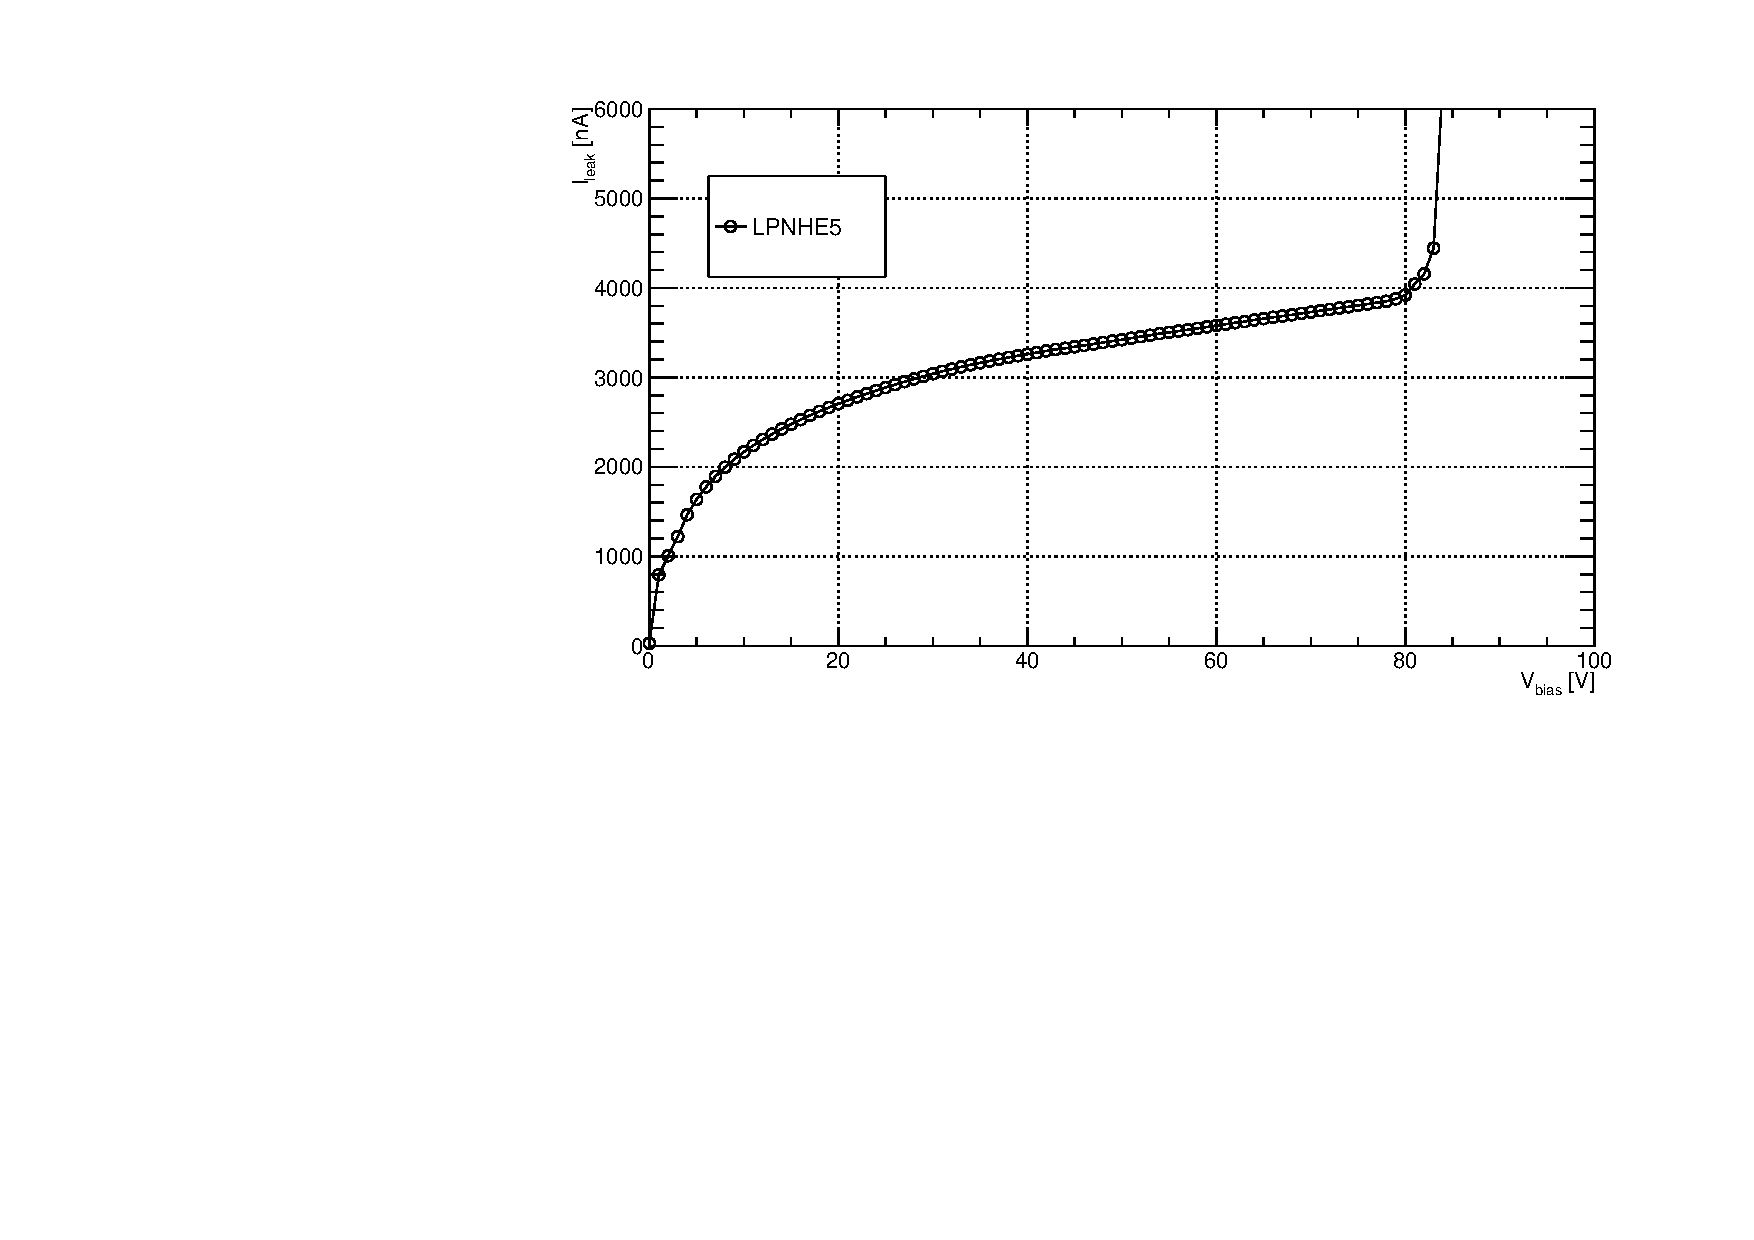
\includegraphics[width=0.55\textwidth]{IV_LPNHE5.pdf}
\caption{\label{fig:IV_LPNHE5}Leakage current as a function of reverse bias voltage for 
a pixel detector. See~\cite{bib:nim2012,2013arXiv1311.1628B}.}
\end{figure}
From Figure~\ref{fig:IV_LPNHE5} it can be seen that a kind of plateau in the current is reached 
between 20 and 80~V; after that voltage the increase in current is huge. Indeed around 80~V 
an {\it avalanche breakdown} occurred. If an electron or hole is created in, or moved into, a high-field 
region inside a semiconductor, it may be accelerated strongly enough in between collisions to obtain 
sufficient energy for the creation of an electron-hole pair: an avalanche may thereafter 
develop~\cite{Lutz:411172}.
Fields higher or of the order of 3$\times$10$^5$~V/cm trigger a multiplication regime that gives rise to a 
breakdown. The voltage at which the phenomenon occurs is called {\it breakdown voltage}.

\section{Why Use Silicon}
\label{sec:Silicon}
Let's know focus only on Silicon. Silicon detectors replaced the  gas based detectors in the tracking systems, since they offer a much
 better position information and an improved energy resolution. The reasons for this are to be found 
in the large density of silicon at room temperature, in the relatively low mean ionisation energy and 
in the possibility of use photolithography to realise charge collecting electrodes. 
These three characteristics allow to have large signals with a small active thickness and 
excellent spatial resolution. Some of the Silicon properties that are relevant for high energy 
physics applications are summarised in Table~\ref{tab:SiProperties}.


% Requires the booktabs if the memoir class is not being used
\begin{table}[htbp]
   \centering
   %\topcaption{Table captions are better up top} % requires the topcapt package
   \begin{tabular}{@{} lcr @{}} % Column formatting, @{} suppresses leading/trailing space
      \toprule
      \multicolumn{3}{c}{Silicon} \\
      \cmidrule(r){1-3} % Partial rule. (r) trims the line a little bit on the right; (l) & (lr) also possible
      Feature    & Value & Comments \\
      \midrule
      \midrule
      Density  $\rho$    & 2.33~g/cm${^3}$ & compact and thin detectors  \\
      Energy bandgap $E_g$ & 1.12~eV & non-cryogenic operation \\
      Mean ionisation energy $\epsilon$ & 3.6~eV & large signals\\
      Radiation length $X_0$      &  9.37~cm & thin detectors to minimize  \\
                                       &                 & multiple scattering \\
      Electron mobility  $\mu_e$     & $\sim$1350 cm$^2$V/s  & fast charge collection \\
      Saturation velocity $v_{sat}$ & $\sim$10$^{7}$ cm/s & fast charge collection \\
      \bottomrule
   \end{tabular}
   \caption{\label{tab:SiProp}Summary of silicon properties relevant for high energy physics applications~\cite{Lutz:411172}.}
   \label{tab:SiProperties}
\end{table}

Other important characteristics that can explain the success of silicon are its large abundance, 
the possibility of changing its properties by doping, the existence of a natural oxide, 
and thanks to its stiffness it does not a container, in contrast to 
gases~\cite{Hartmann2012}.

\section{Silicon Detectors}
\label{sec:Trackers}
We now focus on Silicon ionising particle detectors. They are all based on depleted $p-n$ junctions.  
We will first review the formation of signals and then the different detectors that were and are used 
in high energy physics, in particular those relevant to this report.

\subsection{Signal Formation}
\label{sec:SigForm}

A charged particle traversing the silicon sensor bulk produces electron holes pairs with a most 
probable value (MPV) of 80 pairs per $\mu$m (the energy loss
probability distribution is  described by the  Landau distribution~\cite{Landau:1944if}). 
Because of the sensor's reverse
polarization, the created charge carriers drift toward the sensor electrodes under the influence of
the electric field present in the depleted region. This movement of the charge carriers in the electric 
field induces signals on the readout electrodes.
To calculate the induced signal on the electrodes by the charge carriers drift the Shockley-Ramo 
theorem~\cite{ShockleyPot,Ramo,HE2001250} can be used.
The theorem states that the current $i$ on an electrode induced by a moving point 
charge $q$ is given by:
\begin{equation}
  i(t) =q\vec{v}\cdot\vec{E}_{w}(\vec{r}) 
\end{equation}
where $\vec{v}$ is the instantaneous velocity of charge $q$. $\vec{E}_{w}$ is  the 
electric field that would exist at the instantaneous position $\vec{r}$ of $q$ under the 
following circumstances: the selected electrode at unit potential, all other electrodes at zero potential 
and all charges removed. $\vec{E}_{w}$ is called Ramo field or {\it weighting field}.

The sum of all the induced currents gives the total instantaneous current $I(t)$:
\begin{equation}
I(t) = \sum i(t)=\sum q\vec{E}_w(\vec{r})\cdot\vec{v}_{e,h}(t,\vec{r})
\label{eq:current}
\end{equation}
where the carrier drift velocity is the product of the drift electric field $\vec{E}(\vec{r})$ with the carrier mobility $\mu_{e,h}$:
\begin{equation}
\vec{v}_{e,h}(t,\vec{r})=\mu_{e,h}(\vec{E},T)\vec{E}(\vec{r})
\label{eq:carrierV}
\end{equation}
%As shown in Equation~\ref{eq:carrierV}, the carrier mobility $\mu_{e,h}$ depends on the electric field, the temperature, and the nature of the carrier. 
%Conveniently for the digitizer calculations, the calculation of the induced signal for each charge carrier is completely independent from all the other carriers (see Section~\ref{sec:Athena}).
A carrier that completes its path to the collecting electrode by moving from the position $\vec{r}_i$ where it was created to the
final (electrode) position $\vec{r}_f$ induces the total charge $Q$ given by the Ramo theorem, where 
$V_w(\vec{r})$ represents the {\it weighting} (or Ramo) potential evaluated at the position $\vec{r}$ :
\begin{equation}
Q = - q\left(V_w(\vec{r}_f)-V_w(\vec{r}_i)\right)
\label{eq:signal}
\end{equation}
The relation between the weighting potential and field is of course:

\begin{equation}
\vec{E}_w = - \nabla V_w
\label{eq:weightrel}
\end{equation}

A carrier $q$ that is produced at position $\vec{r}_i$ and trapped at position $\vec{r}_f$, before 
reaching the electrode, induces a smaller charge $Q$ on the electrode by the same formula 
(carrier trapping will be presented in detail in Section~\ref{sec:trapping}). It has to be noticed that both 
trapped electrons and trapped holes reduce the final signal amplitude.

\subsection{Pad detectors}
\label{sec:pads}

We now consider $p-n$ junction {\it diodes}.
A single p-n diode in reverse bias is the simplest silicon radiation detector; 
often it is called {\it pad} diode. Ionising  particles interacting with  the detector material 
produce electrons and holes in the depleted bulk volume; those carriers drift toward 
the collecting electrodes which are placed at the edge of the detector $p-n$ junction. 
To ensure 
a good ohmic contact heavily doped implants are present on both sides of the detector. 
In Figure~\ref{fig:pad} the schematic representation  of a n-on-p pad diode silicon detector is 
shown. External voltage to ensure sensor bulk depletion is also indicated.  


\begin{figure}[!htbp]
   \centering
   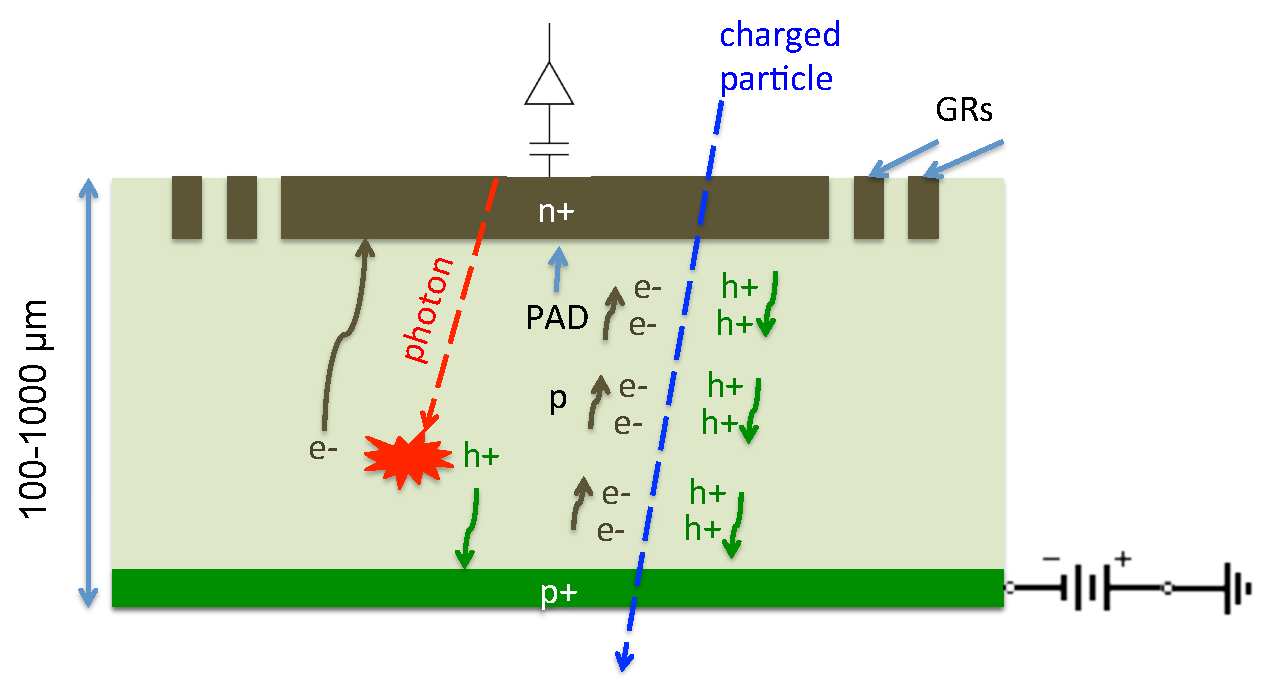
\includegraphics[width=0.5\textwidth]{pad.pdf} 
  % 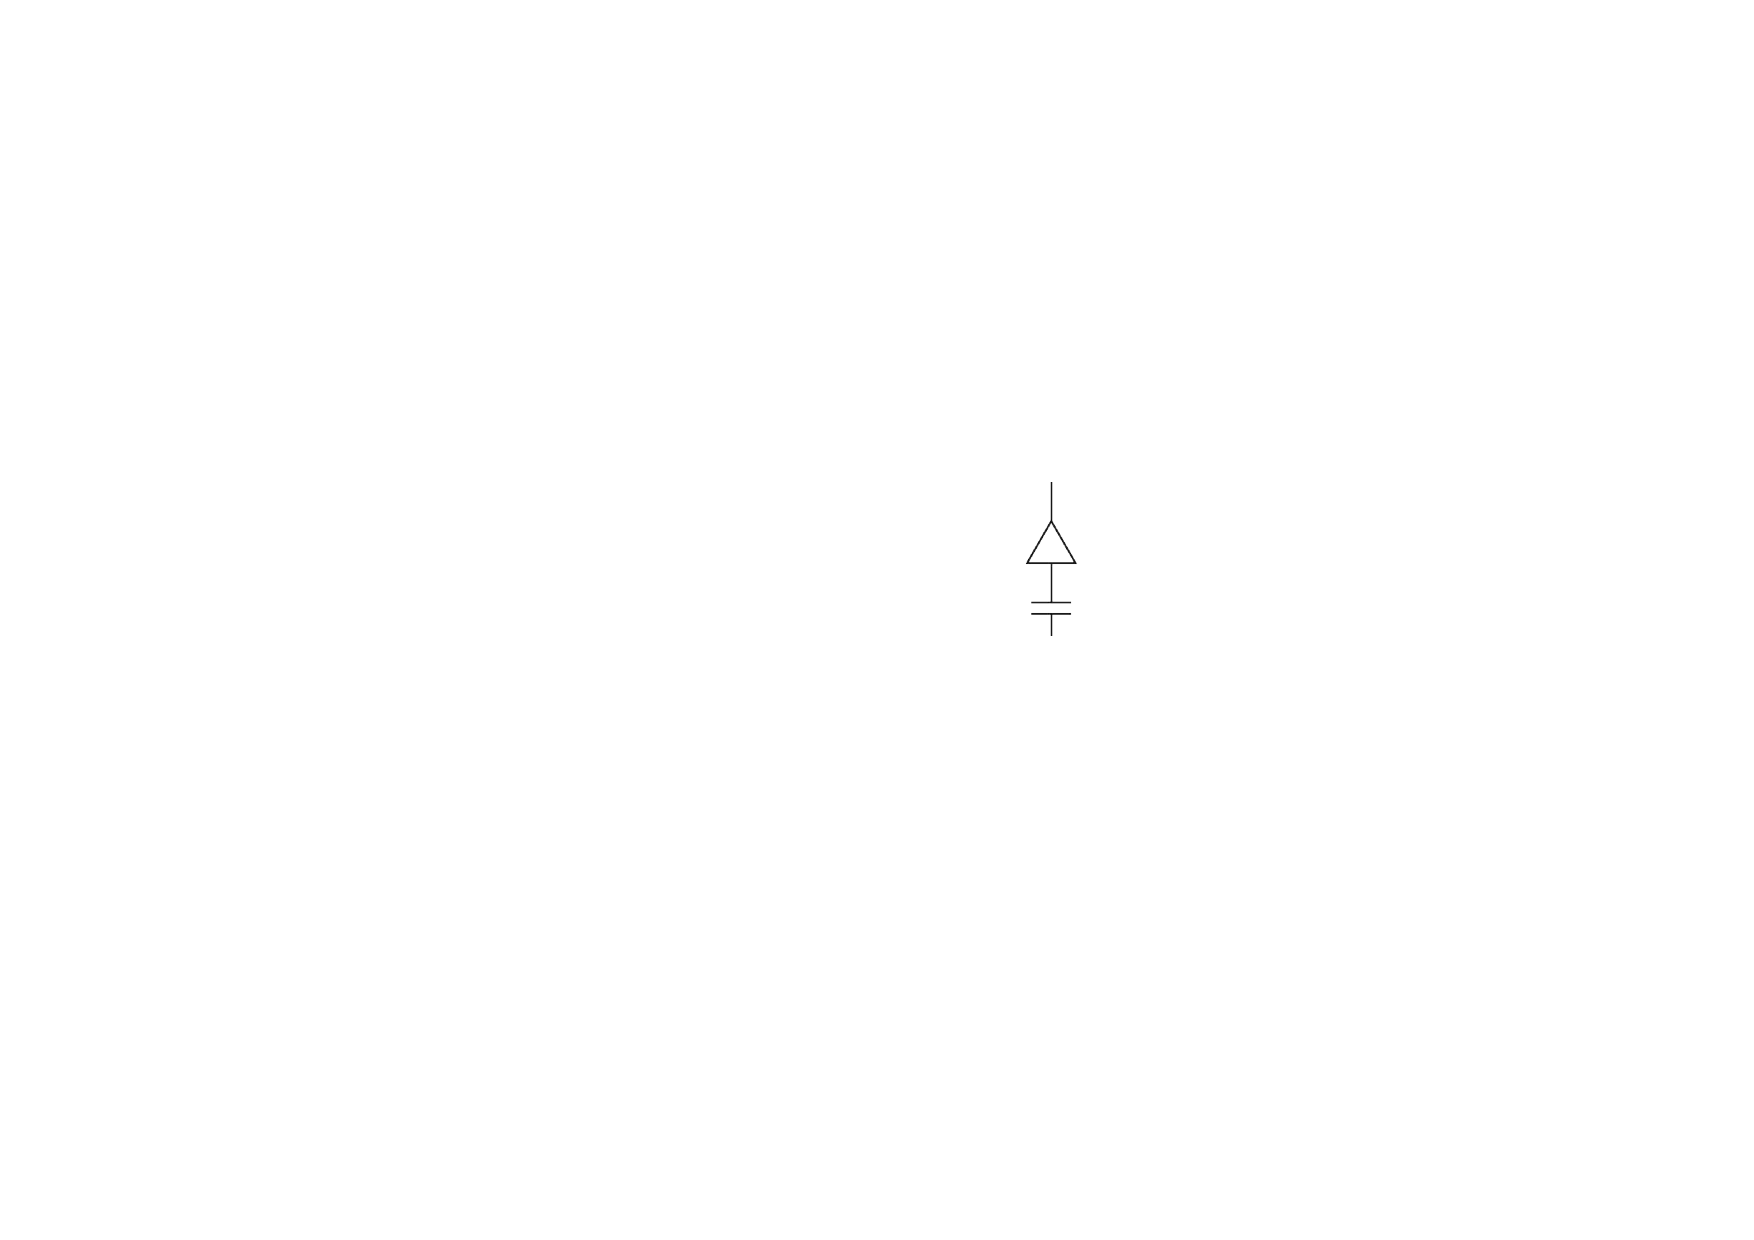
\includegraphics[width=0.07\textwidth]{ro.pdf} 
      \caption{\label{fig:pad} Silicon pad detector. Detector polarisation and carrier drift due to 
      ionising particles is indicated too. The symbol on top of the $n^+$ implant is used to indicate the 
      readout electronics.}
\end{figure}
%Charged particles at the minimum of ionisation creates about 100 electron-hole pairs per $\mu$m of 
%traversed Silicon. The drift of these charges induce a signal into the electrodes. 
The size of pad detectors varies between few mm$^2$ to few cm$^2$,
including Guard Rings (GRs).  GRs, placed all
around the pad area, can help to improve the voltage-handling capability, since they act as a 
voltage divider, assuring a smooth transition of the voltage drop between one side 
and the other of the junction. 
Normally in pad diodes signals are read-out only from one side of the junction; it is customary 
to call that side as {\it frontside}, the other being the {\it backside}. 
For example, in Figure~\ref{fig:pad} the 
frontside is the $n^+$ one.

The pad side from which the depletion volume grows is called {\it junction} side; the other 
one is indicated as the {\it ohmic} side.

\subsection{Microstrip detectors}
\label{sec:microstrips}
The spatial resolution of pad detectors is roughly the size of the pad itself.
 It can be greatly improved by segmenting the electrodes, just one of 
them or both. 
  Historically the first segmented silicon detector for high energy physics purpose was created by 
 aluminum strips deposited on a silicon wafer~\cite{Amendolia}. 
Nowadays so called {\it microstrip} detectors are realised by creating an array of heavily doped 
strips crossing the surface 
 of the lightly doped silicon bulk. Each strips is read independently as shown in Figure~\ref{fig:strips}.
 
 \begin{figure}[htbp]
   \centering
   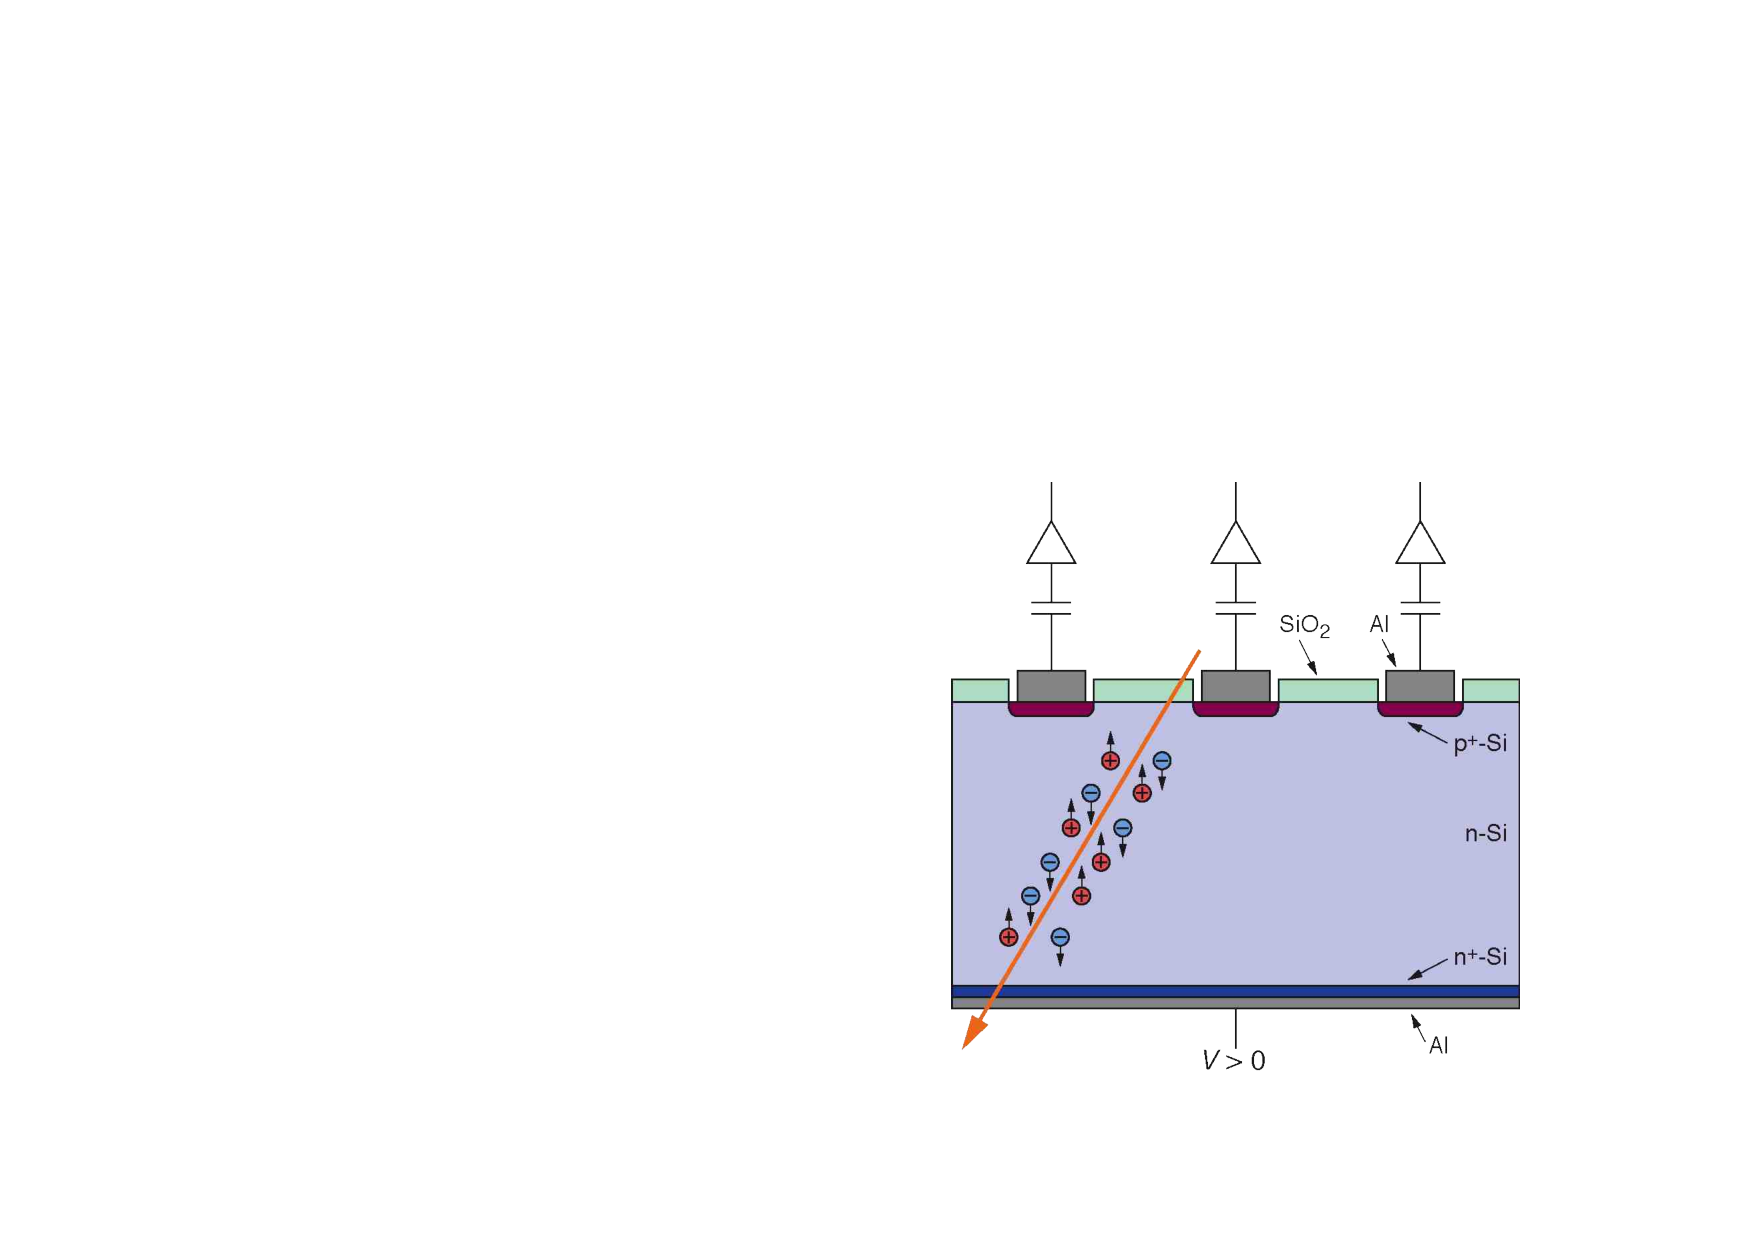
\includegraphics[width=0.4\textwidth]{Strips.pdf} 
      \caption{\label{fig:strips} Silicon microstrip p-on-n detectors sketch. (After~\cite{Krammer})}
\end{figure}
 
 The typical spatial resolution of these detectors is of the order of (a fraction of) the strips pitch 
 (50-80~$\mu$m nowadays).
 Adding one floating strip ({\it i.e.} not connected to a readout channel) can greatly 
 improve the spatial resolution without increasing the number of channels to be 
 readout~\cite{TURCHETTA}. We will come back to the strip detectors and their spatial resolution in 
 more detail in 
 Section~\ref{sec:striplets_res}.
 
 Microstrip detectors where  the ohmic side is segmented too  are called {\it double-sided microstrip 
 detectors} (DSSDs); a scheme presenting the salient features of the DSSDs is shown in 
 Figure~\ref{fig:DSSD}
  \begin{figure}[htbp]
   \centering
   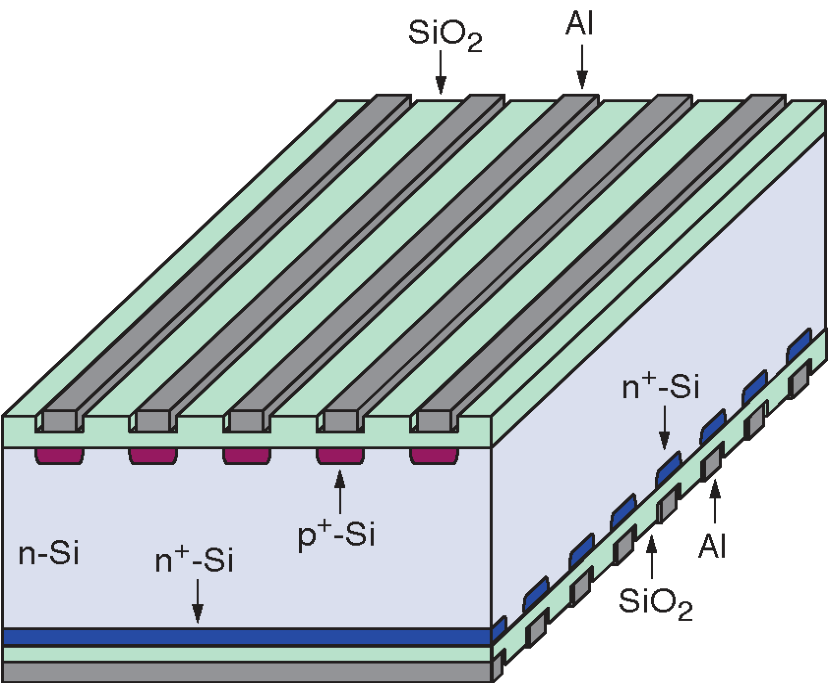
\includegraphics[width=0.35\textwidth]{DSSD.pdf} 
  % 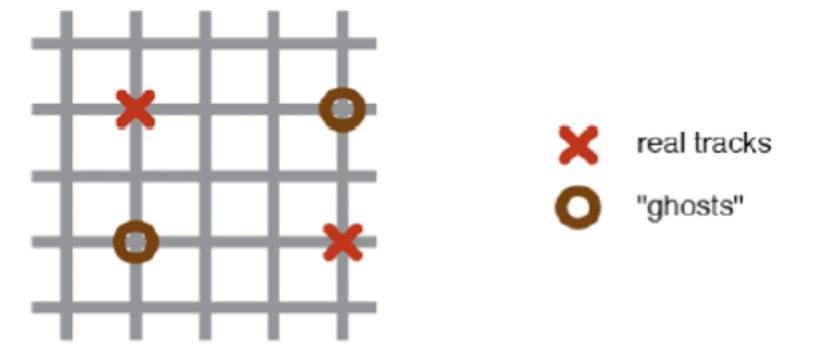
\includegraphics[width=0.5\textwidth]{DSSD_and_Ghosts.pdf} 
      \caption{\label{fig:DSSD} Schematic representation of a DSSD. (After~\cite{Krammer})}
\end{figure}

  DSSDs allow the reconstruction of two coordinates in one detector layer; 
 this is very important to avoid deteriorating too much the spatial resolution 
 due to the multiple scattering. 

One important limitation of the DSSDs is the non unambiguous particle position measurement when 
more than one track is hitting the detector at the same time. As shown in the example 
in Figure~\ref{fig:ghosts}, when two tracks hit the detector two valid but spurious combinations 
appear (``ghosts''),  other than the two ``true' valid positions due to the real tracks.

  \begin{figure}[htbp]
   \centering
  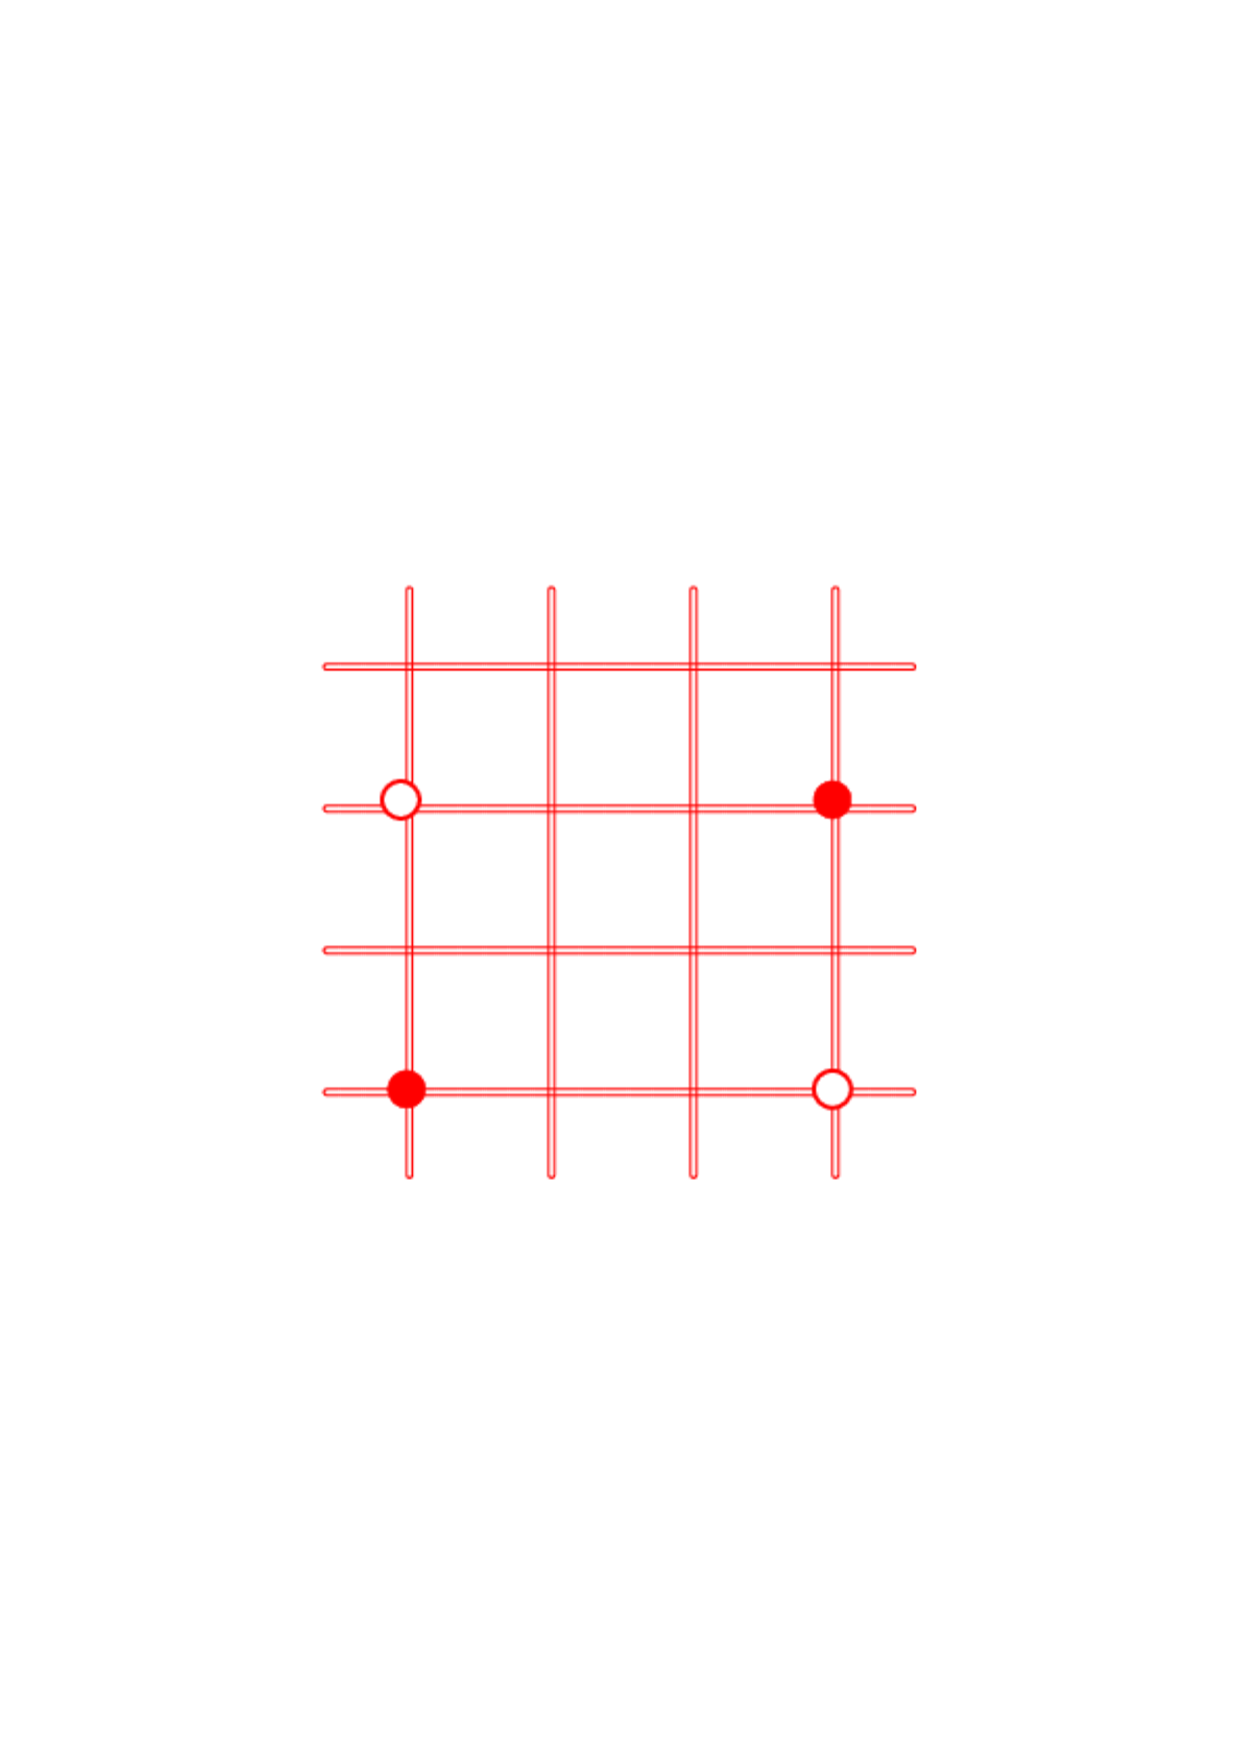
\includegraphics[width=0.35\textwidth]{ghosts.pdf} 
      \caption{\label{fig:ghosts} Schematic representation of the formation of ghost hits in 
     DSSDs. The incidence positions of two particles are indicated as  red 
      crossed. Two additional valid combinations of the 1D information of both sides are indicated 
      as brown open circles. Strips in red are those who recorded a signal. (After~\cite{Krammer})}
\end{figure}


\subsection{Pixel detectors}
\label{sec:pixels}
To measure unambiguously the position where the tracks cross the detector a detector capable 
of delivering both coordinates in one single measurement is needed: a {\it pixel} detector~\cite{Pixels}.
The concept of {\it hybrid pixels} detectors (HPDs) is presented in Figure~\ref{fig:pixels}. 
 \begin{figure}[htbp]
   \centering
  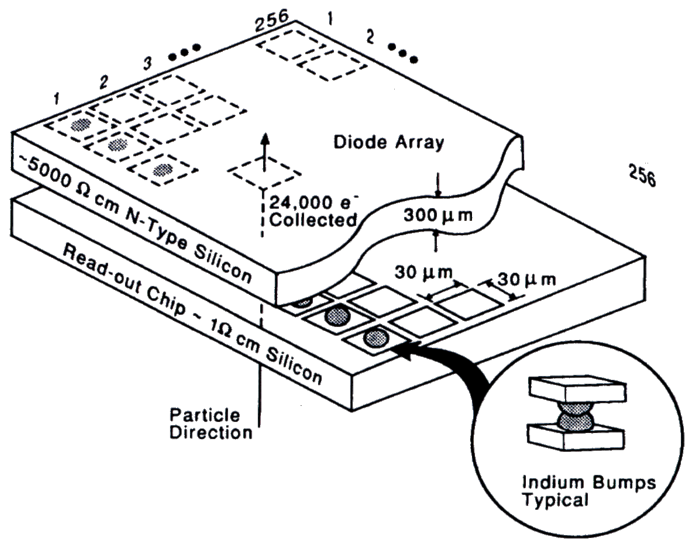
\includegraphics[width=0.35\textwidth]{HPD.pdf} 
    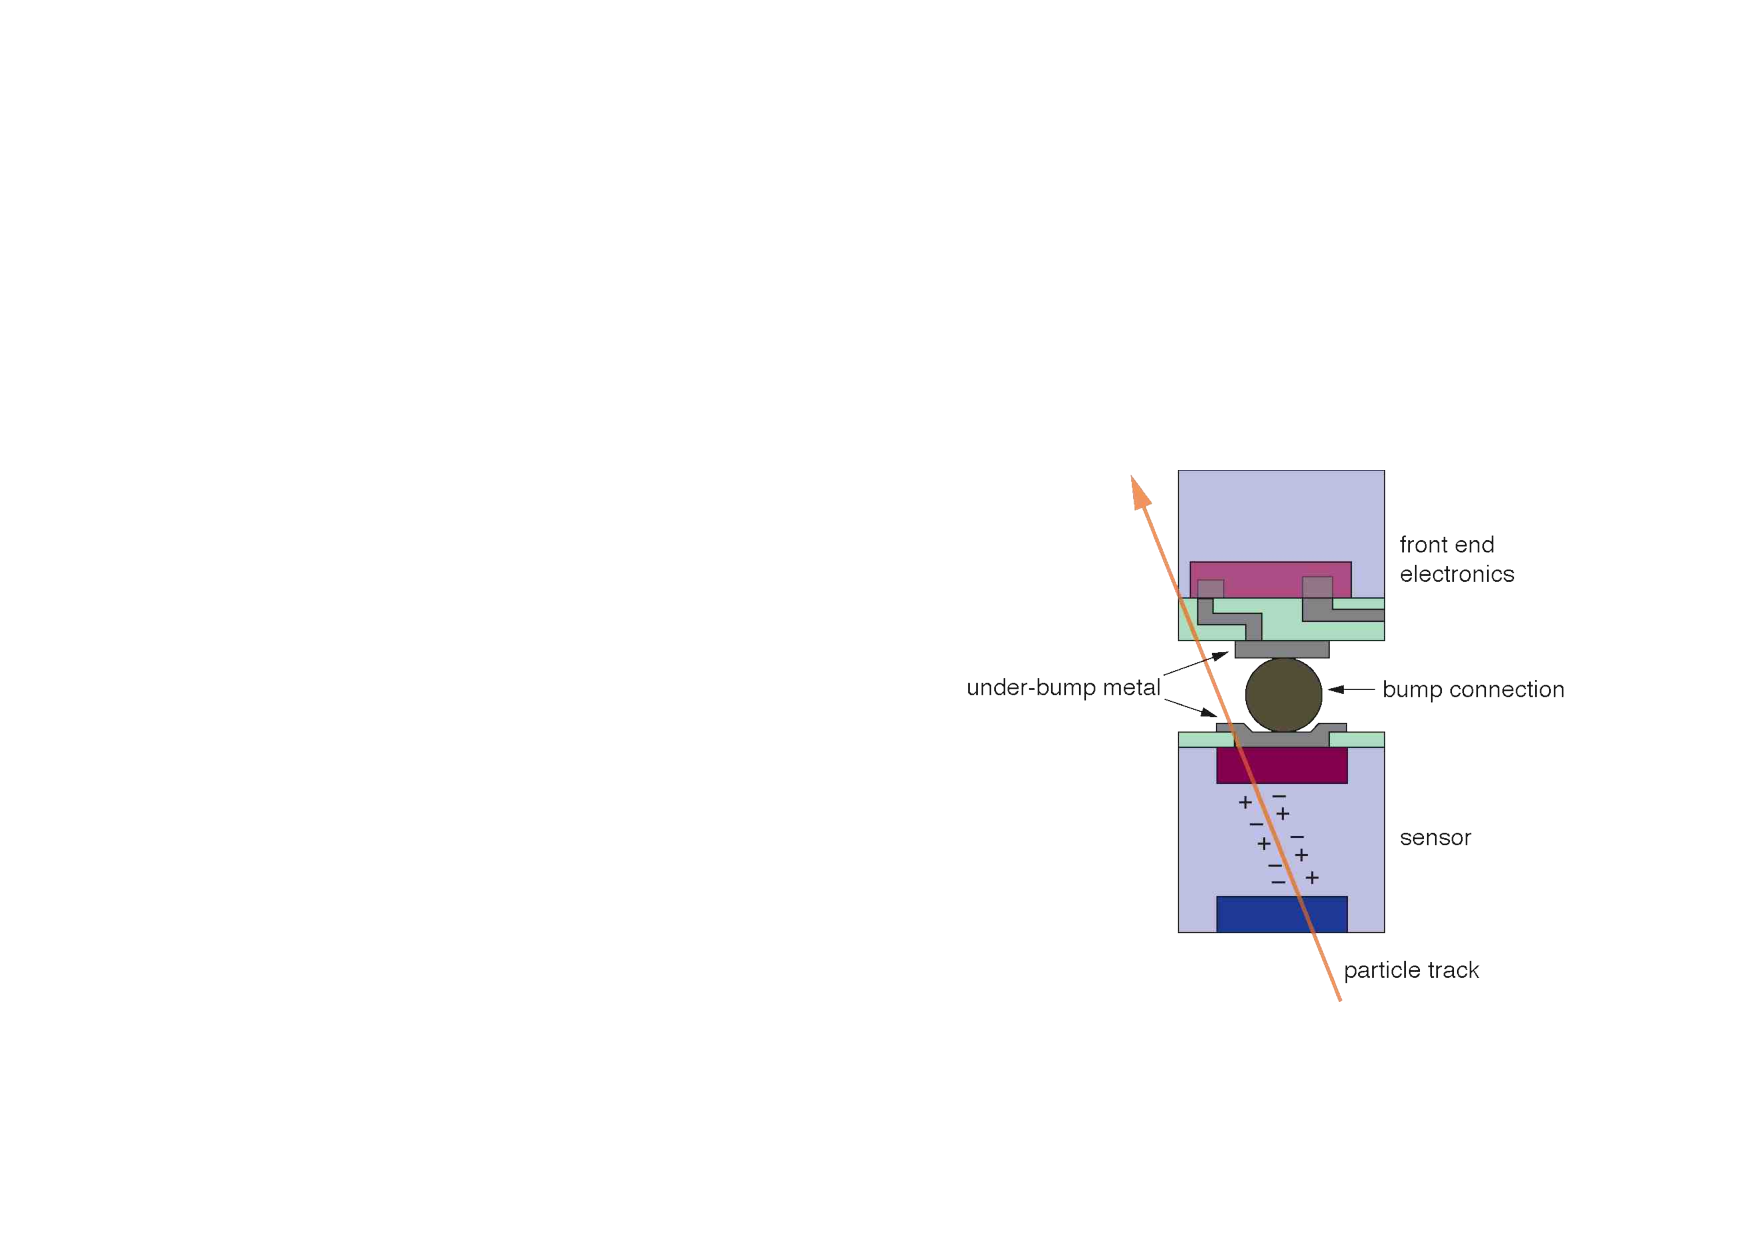
\includegraphics[width=0.35\textwidth]{pixel_bb_roc.pdf} 
      \caption{\label{fig:pixels} Schematic representations of an hybrid pixels detector. (Left) array 
      of silicon $p-n$ diodes organised into a pixel detector. Each pixel cell is readout by a dedicated 
      channel of the front-end electronics.(Right) detail of one pixel sensor cell connected via bump 
      bonding to its front end electronics channel. (After~\cite{Pixels,Pixels2003})}
\end{figure}
A two dimensional array of $p-n$ diodes are organised in a matrix; each $p-n$ junction is readout 
by a dedicated  readout integrated circuit (ROIC), providing the functionality of a hybrid pixel assembly; 
hence sensor and readout electronics are physically separated 
and linked by a {\it bump bonding}. The term {\it hybrid} refers to the fact that sensor and electronics 
are built onto separate substrates then joint together indeed by means of the bump bonding technique.
The typical pitches of nowadays HPDs are of the order of 
 $50$~$\mu$m in the direction perpendicular to the magnetic field (``bending plane'') and 
 a couple of times larger in the beam direction.
 

 
 HPDs, other than unambiguous position measurement, compared to DSSDs offer 
 smaller leakage current (few pA) and smaller capacitance (few fF) per channel, 
 given the much smaller size of the 
 fundamental sensor cell; both aspects help in keeping the level of electronic noise small, hence 
 to preserve high detector efficiency and spatial resolution.
 The main limitation of HPDs is the elevated number of channels to be readout ({\it e.g.}$\sim$27000 
 in $\sim$ 4~cm$^2$~\cite{IBLTDR}). 
 The high number 
 of readout channels gives rise to complex solutions for sensor-electronics connection and 
 large power consumption (0.1-1 W/cm$^2$~\cite{IBLTDR}).

A variation of the sensor of HPDs are the so-called 3D-silicon sensors. 3D-silicon sensors have been 
developed since the late 1990s~\cite{PARKER1997328} 
featuring columnar electrode implants driven into the Si substrate perpendicular to the sensor surface 
(Figure~\ref{fig:tredi}).

 \begin{figure}[htbp]
   \centering
  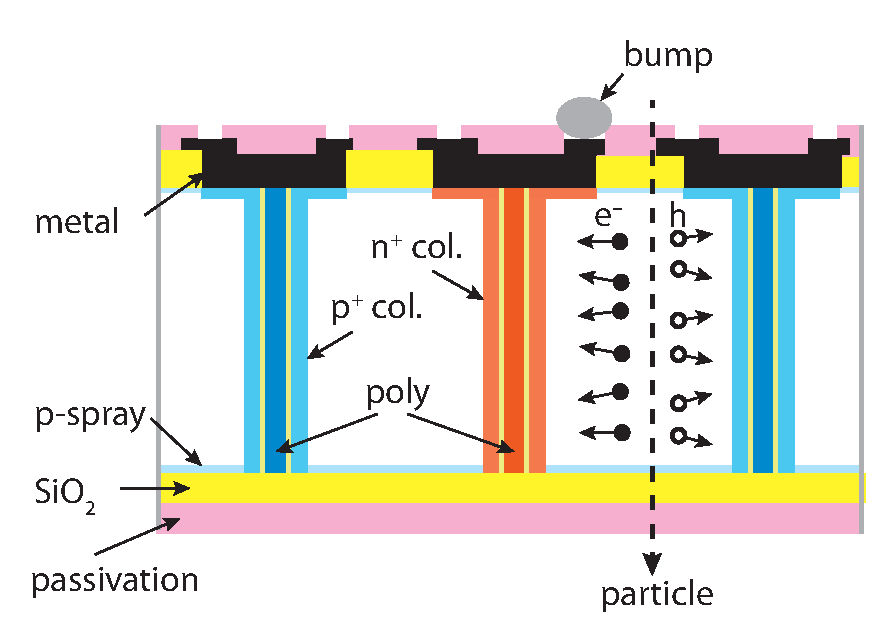
\includegraphics[width=0.45\textwidth]{tredi.pdf} 
      \caption{\label{fig:tredi}Single sided 3D-Si sensors with columns going completely through the 
      sensor bulk. (After~\cite{Garcia-Sciveres:2017ymt})}
\end{figure}
The electrode distance is made smaller (50~$\mu$m) than the typical sensor thickness 
(200-250~$\mu$m), thus rendering a shorter average drift distance for particles impinging on the sensor 
face than in the case of planar sensors. In addition high drift fields are obtained with still moderate bias 
voltages. Both these facts result in an increased radiation tolerance due to a reduced trapping 
probability (see~\ref{sec:trapping}).

\subsection{Monolithic Pixel Detectors}
\label{sec:MAPS}
The high number of interconnections and the total material budget are the main limitations imposed 
by the HPDs. One solution is to have on the same substrate the sensor and the  frontend electronics: 
 simple electronics circuits, like the first stage of the amplifier of each pixel, are integrated on the 
 same silicon substrate. 
 One example of sensor and frontend electronics integrations are the Monolithic Active Pixel Detectors 
 (MAPS~\cite{CLAUS2001120}), which are realised  in  
 commercial CMOS technology (for CMOS technology see for example~\cite{Lutz:411172}).  
 The detector is realised on a thin layer of low-resistivity $p$-doped silicon, which is optimal for complex 
 electronics design but does not allow having large depletion volumes and fast charge 
 collection~\cite{rossi2006pixel}. The conceptual drawing of an example of MAPS is presented 
 in~\ref{fig:maps}.
 \begin{figure}[htbp]
   \centering
  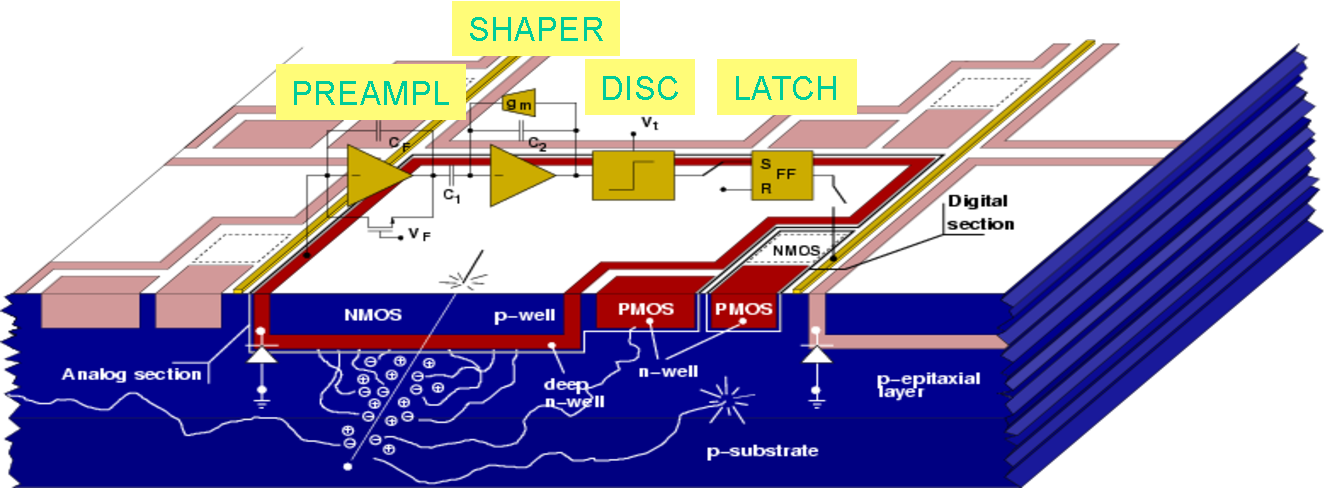
\includegraphics[width=0.55\textwidth]{maps.pdf} 
      \caption{\label{fig:maps} Conceptual drawing of an example of MAPS (After~\cite{ReApsel})}
\end{figure}
The $p-n$ junction is realized between the n-well and the $p-$type epitaxy\footnote{epitaxy is 
semiconducting material made by epitaxial growth}, but, because of the low resistivity, the depletion is 
partial even on the very thin ($\approx$10~$\mu$m) epitaxy layer and the collected charge is small 
($\approx$1000e). The 
charge collection from the epitaxial layer to the n-well/p-epi diode happens through drift and diffusion of 
the carriers and takes about 100~ns, {\it i.e.} 10 times longer than in the approaches based on 
high-resistivity silicon.

%Even as monolithic solutions mature, hybrid technology with special purpose ROICs will continue to be 
%necessary for the highest rate capability and the implementation of new functionality, such as fast 
%timing. Looking to industry we find that the monolithic CMOS sensors in modern smartphones are 
%actually 3D integrated devices~\cite{Garcia-Sciveres:2017ymt}. 

Modern CMOS imaging sensors make use of 3D integration to combine high resistivity and 
fully depleted charge collection layers with high density CMOS circuitry, in order to achieve high speed 
and high collection efficiency (for low light operation). Such a combination of fully depleted high 
resistivity silicon with CMOS readout sounds like a requirement from particle physics, not from 
consumer electronics, but smartphone image sensors have independently evolved in this 
direction. Recently depleted monolithic active pixel sensors 
(DMAPS) started to be developed; they exploit medium to high (>100$\Omega$cm) resistivity 8" silicon substrate wafers. A depletion layer develops due the high resistivity with only moderate bias voltages applied from the electronics side or a (specially processed) backside 
contact~\cite{Garcia-Sciveres:2017ymt}.

\section{Radiation Damage}
\label{sec:RadDam}

Silicon detectors are at the core of the modern High Energy Physics (HEP) experiments at colliders. 
High collision rates 
and high track densities translate into fluence of particles of several $10^{11}$ per square centimetre 
per hour for the detector layers closest to the interaction point~\cite{rossi2006pixel}. This flux of 
particles is responsible for damage to the sensor and to the electronics. 

Radiation-induced effects (radiation damage) are usually divided into bulk and surface defects. The 
former are caused by the displacement of crystal atoms while the latter include all effects in the 
covering dielectrics and the interface region. The most important surface effect is the increase of the 
oxide charge which saturates after some kilograys to values of about 10$^{12}$~cm$^{-2}$~\cite{Oldham}. 
At higher hadron fluence, bulk damage also becomes important. The main effects are: increase of 
leakage current, change of the operational voltage and reduction in signal amplitude. 
The following is a short description of the microscopic defects and the induced macroscopic effects.

\subsection{Microscopic description}
Inelastic collision between an incident particle and the silicon lattice can produce a displacement 
of an atom from its lattice site. This event creates an interstitial site and a vacancy, which 
collectively is called a {\it Frenkel defect}. An illustration of these defects, called also {\it point defects}, 
is give in Figure~\ref{fig:Interstitial}.


\begin{figure}[!htbp]
\centering
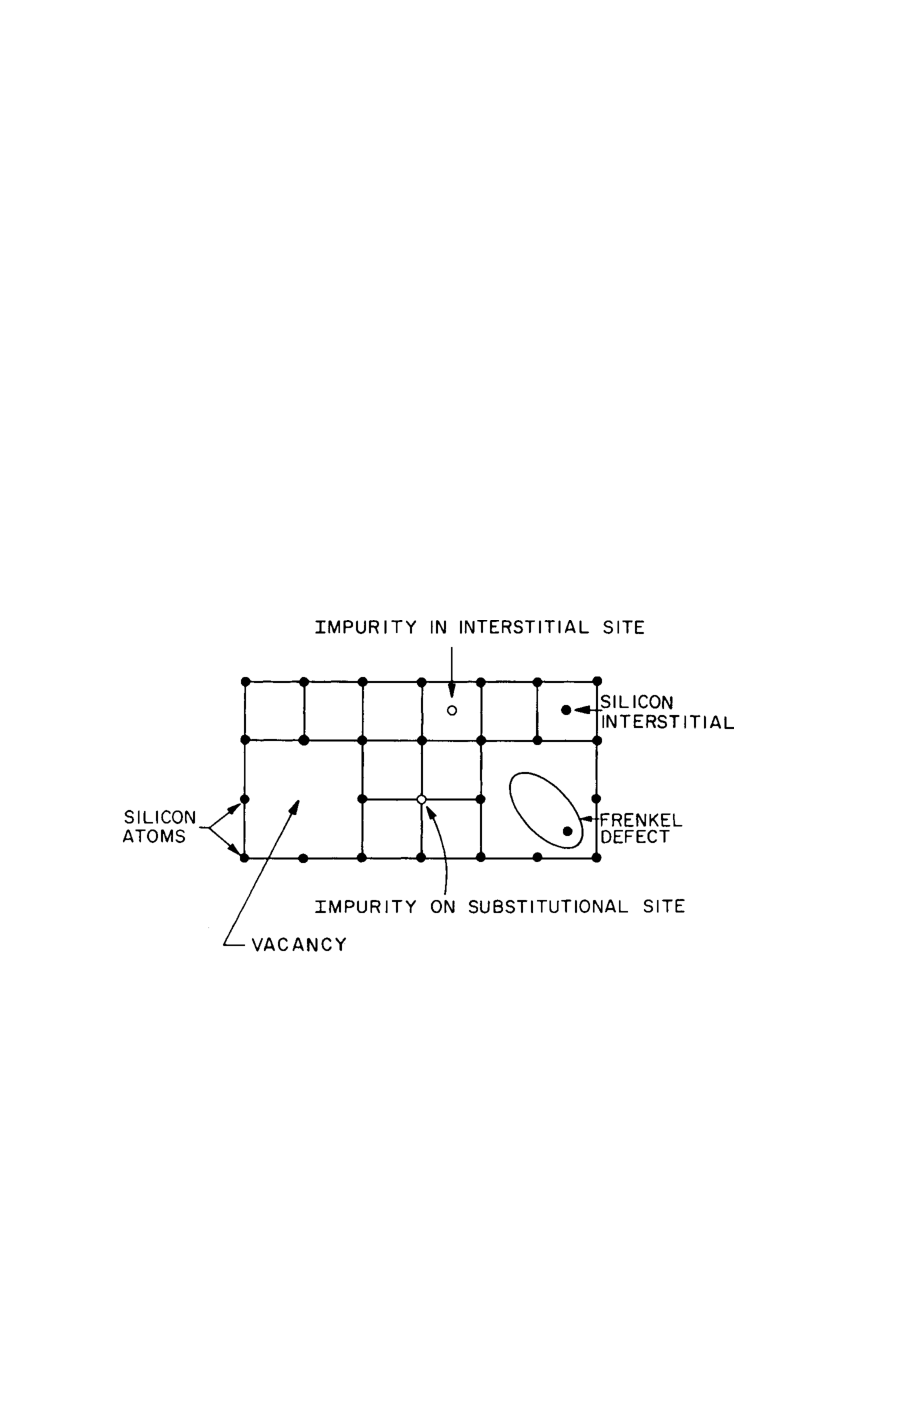
\includegraphics[width=0.5\textwidth]{Interstitial.pdf}
\caption{\label{fig:Interstitial}Types of point defects in a simple lattice. After~\cite{Lutz:411172}.}
\end{figure}


Several point defects can group together to form a cluster; the probability 
depends on the incident particle type and its energy. 
An electron whose kinetic energy is above 255~keV produce a Frenkel pair; above 8~MeV it 
produces a cluster. For neutrons the thresholds are of 185~eV and 35~keV, 
respectively~\cite{moll-thesis}. In Figure~\ref{fig:clusters} the results of a Monte Carlo simulation 
for the recoil of an atom with a primary energy $E_R$ of 50~keV; this is the average energy imparted 
to a lattice atom from a 1~MeV neutron~\cite{moll-thesis}.


\begin{figure}[!htbp]
\centering
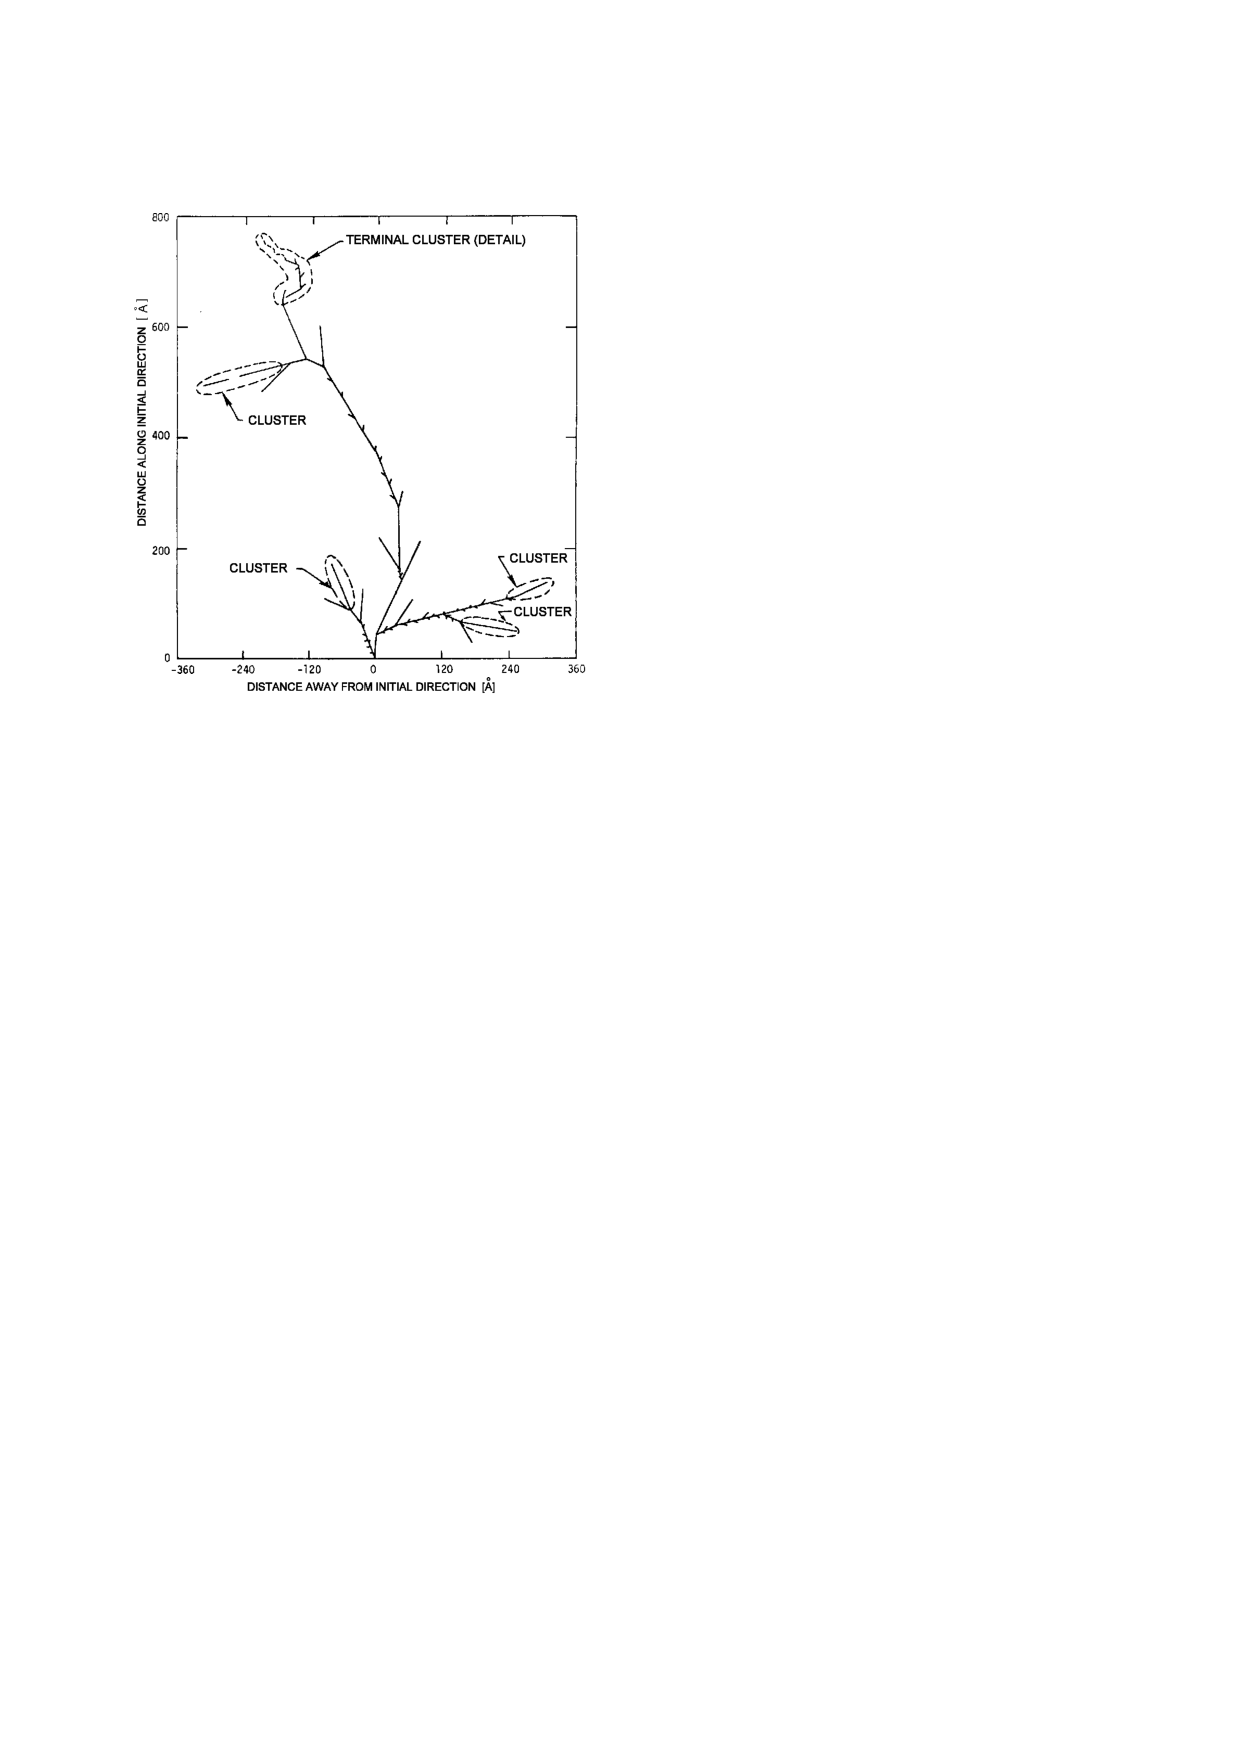
\includegraphics[width=0.5\textwidth]{clusters.pdf}
\caption{\label{fig:clusters}Monte Carlo simulation of a recoil-atom track with a primary energy $E_R$
of 50~keV. After~\cite{van1980mechanisms}.}
\end{figure}

To be able to compare the damage caused by the different types of particles with different energies, 
radiation damage is scaled with the non-ionizing energy loss (NIEL). This quantity summarises all 
energy deposited in the crystal which has not been used for the fully reversible process of ionisation. 
Neutrons of 1~MeV are used as reference particles~\cite{astm}. The fluence $\Phi_{\rm phys}$ of an arbitrary type 
of particle causes the same NIEL as the fluence $\Phi_{\rm eq}$ of 1~MeV neutrons.
The energy-dependent hardness factor $\kappa$ of a certain type of particle which converts the 
``physical'' fluence $\Phi_{\rm phys}$ into the neutron equivalent fluence $\Phi_{\rm eq}$ can be 
evaluated experimentally via the normalisation of the leakage 
current~\cite{MOLL2002100,rossi2006pixel}. In the following text all fluences are given in units of neutron equivalent fluence, n$_{\rm eq}$/cm$^2$. 

The primary defects caused by irradiation, silicon vacancies, and interstitials are not stable; {\it i.e.}, 
they 
are able to move through the crystal. This movement can lead to an {\it annealing} if defects 
meet during 
their migration through the crystal. But also secondary point defects with other defects already present 
in the crystal can be formed, which might be stable and display different electrical properties. Point 
defects in general cause energy levels in the band gap whose position can be measured by different 
spectroscopic methods. They can be charged and, depending on the position of their energy levels, 
have an impact on the space charge in the depletion zone. As the mobility of the defects is strongly 
temperature-dependent it is clear that radiation-induced changes of sensor properties show a complex 
annealing behaviour due to the many possible secondary defects~\cite{rossi2006pixel}.


Among several defects detected with various techniques, there are some that prove to have a significant impact
on the silicon diodes, being charged at ambient temperatures and thus, directly influencing the 
effective doping concentration $N_{eff}$. Their electrical parameters, energy level $E_a$ 
and capture cross section $\sigma$ are given in Figure~\ref{fig:Defects}~\cite{DefectsVertexing2016}.

\begin{figure}
\centering
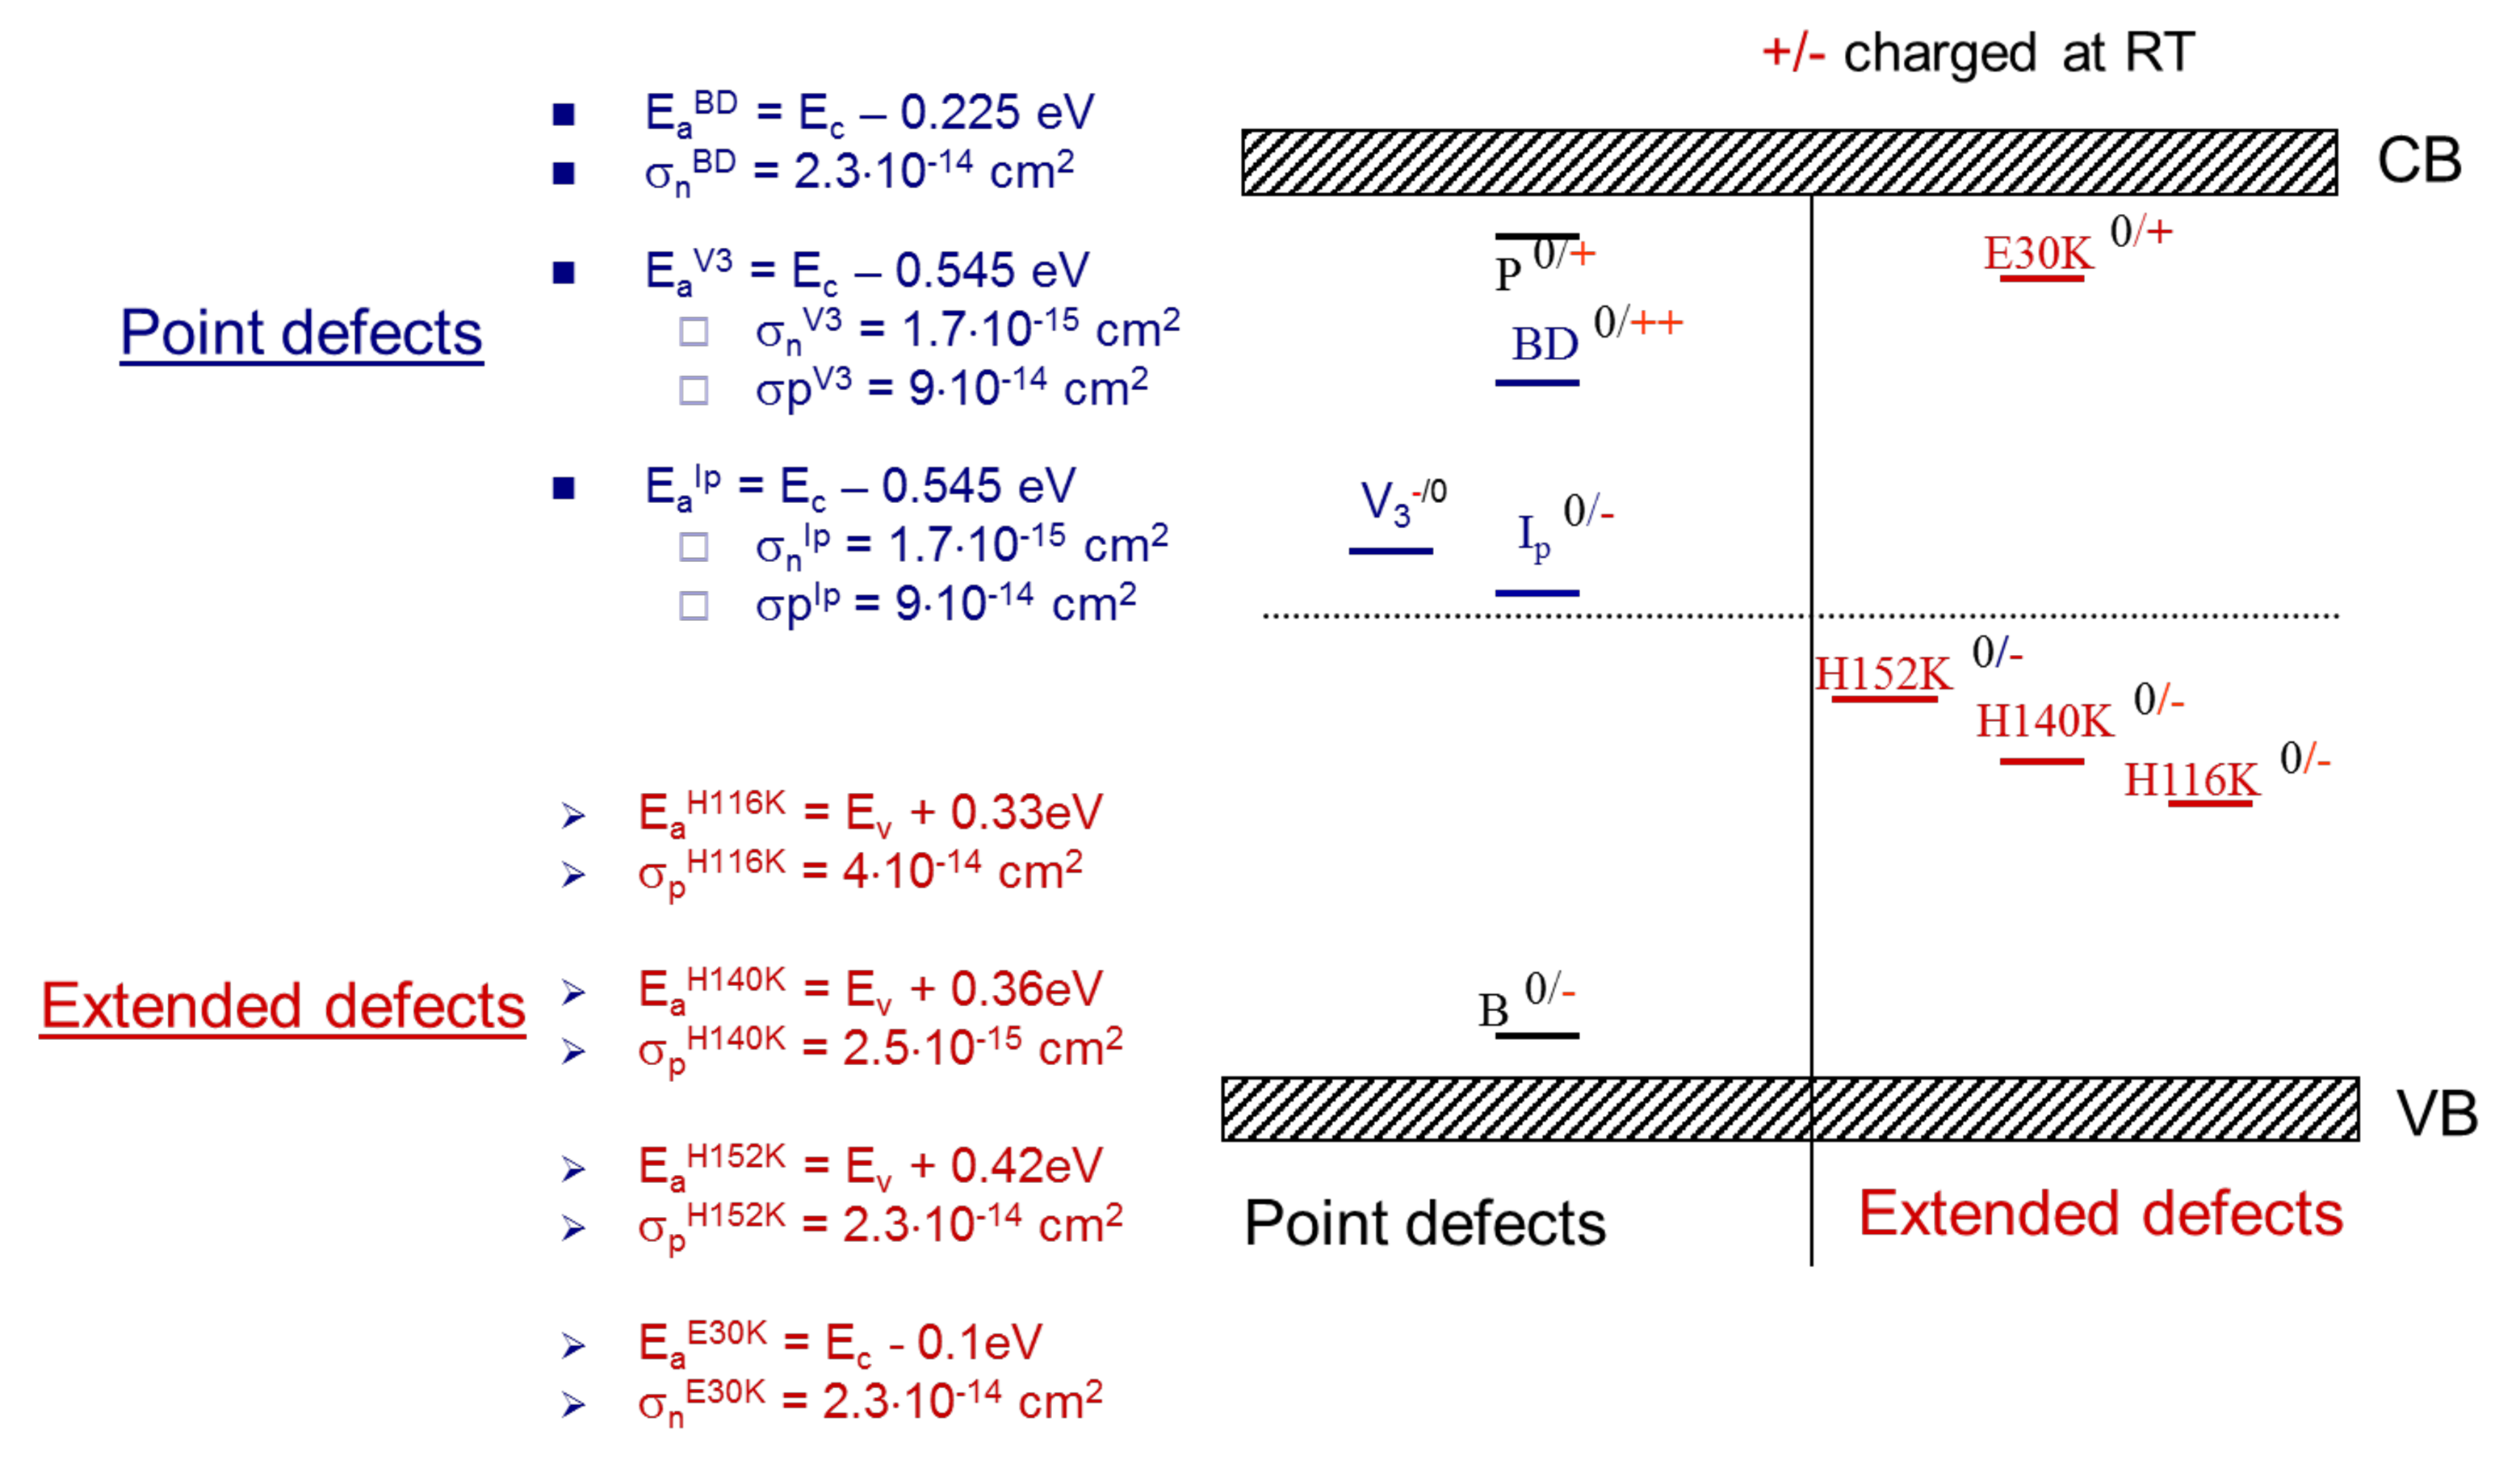
\includegraphics[width=0.65\textwidth]{Defects.pdf}
\caption{\label{fig:Defects}Radiation induced defects in silicon influencing  the  effective doping 
concentration $N_{eff}$ and the leakage current. $P$ and $B$ are the doping impurities
used to fabricate the silicon $p-n$ junctions. $CB$ and $VB$ stand for conduction and valence bands, 
respectively. (After~\cite{DefectsVertexing2016})}
\end{figure}

The radiation induced defects, primary or not, are responsible for macroscopic effects, like: the increase 
of leakage current, since they can act as generation centers; the change in operational voltage, as they 
can be charged; and, the most important effect after $\Phi$=$10^{15}$~n$_{\rm eq}$/cm$^2$, the 
reduction of the signal amplitude, since they act as trapping centers. Let's now review some details 
of these macroscopic effects.

\subsection{Leakage Current Increase}
The energy levels in the band gap caused by the crystal defects act as generation-recombination 
centers. 
They lead to a decrease of the generation lifetime $\tau_g$, hence to an increase of the leakage 
current $I_{leak}$ generated in the volume. The rate of increase of leakage current $\Delta I$ per unit of 
fluence $\Phi$ and per unit of volume $V$ is called $\alpha$:

\begin{equation}
\alpha = \dfrac{\Delta I}{V\Phi}
\label{eq:alpha}
\end{equation}
 
 The typical value of the normalised rate of increase of leakage current $\alpha$ right after irradiation is of several units of $10^{-17}$~A/cm. After 
 irradiation the leakage current anneals with time as shown in Figure~\ref{fig:alpha_annealing}.
 
 \begin{figure}[!htbp]
 \centering
 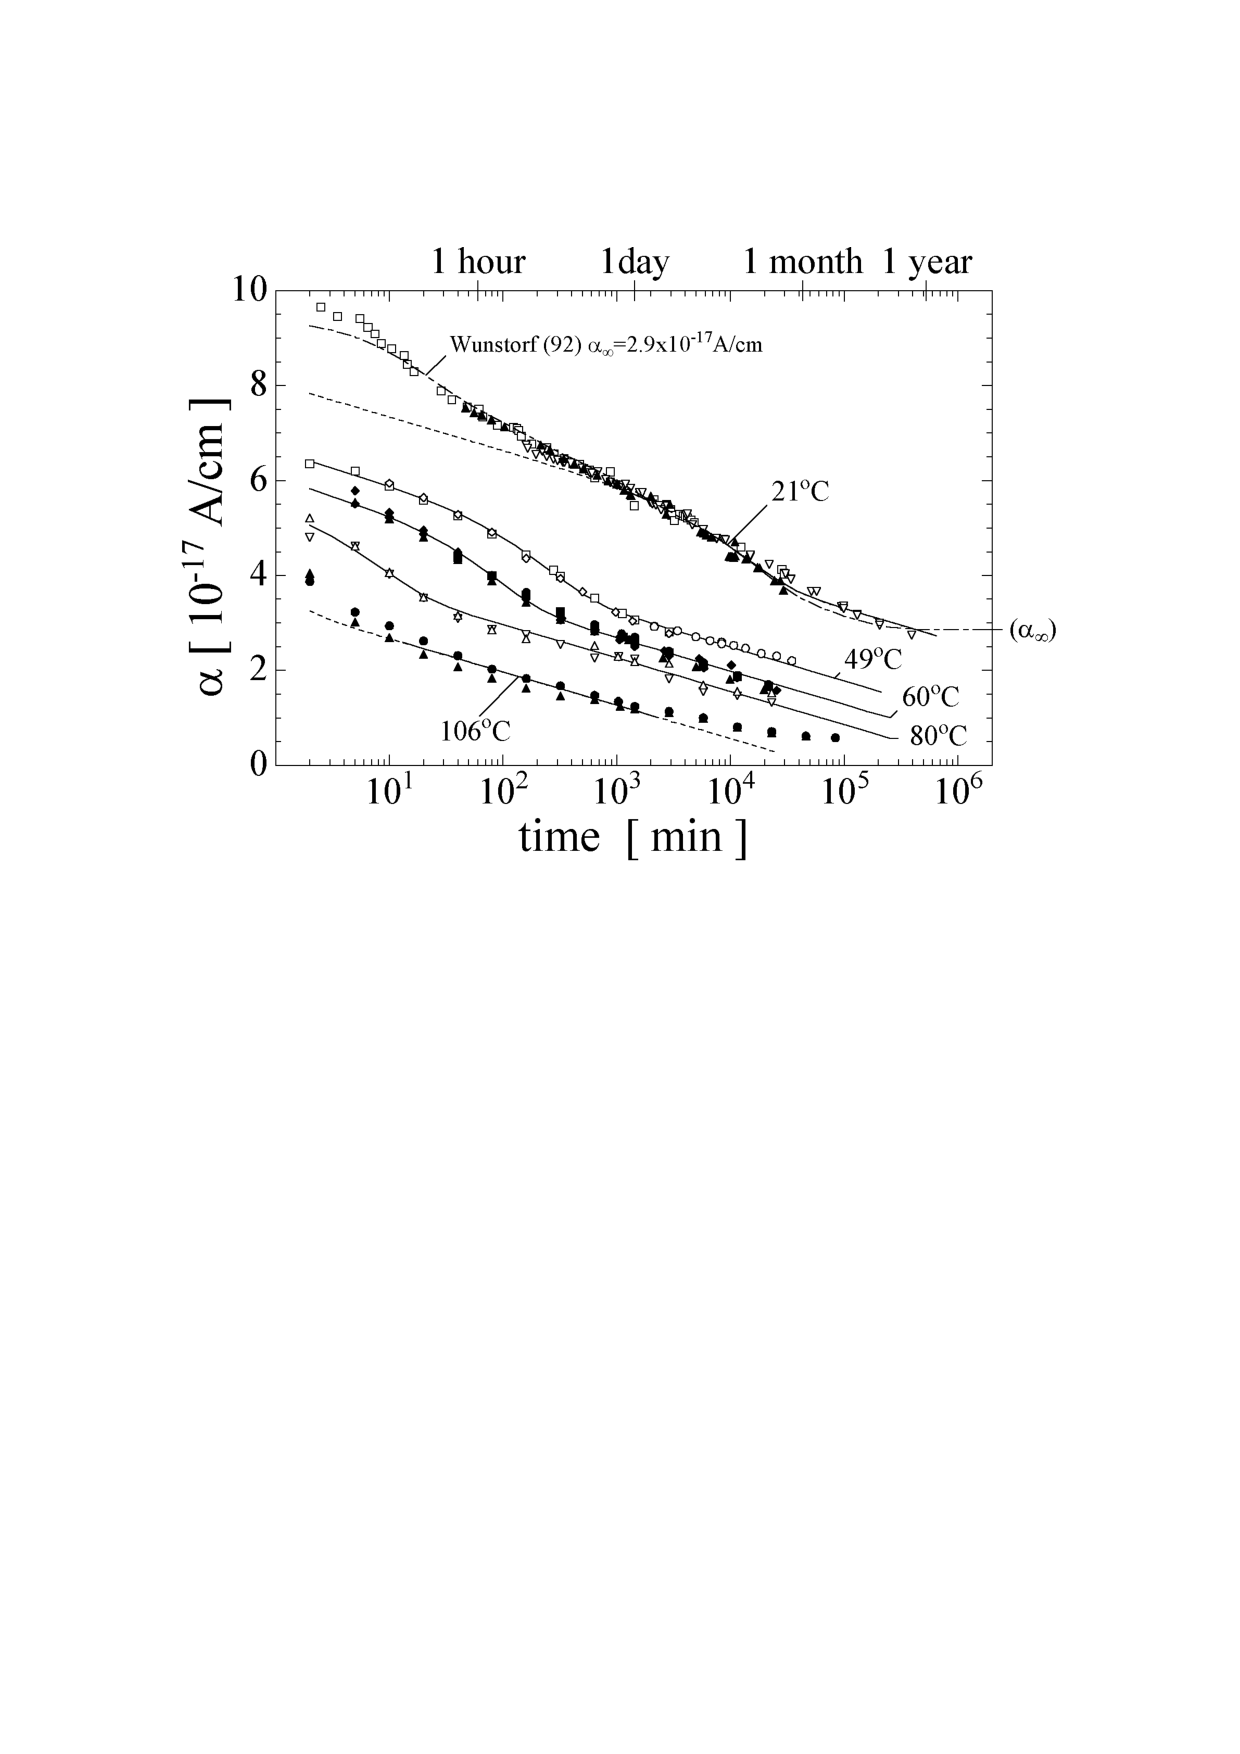
\includegraphics[width=0.5\textwidth]{alpha_annealing.pdf}
 \caption{\label{fig:alpha_annealing}The normalised rate of increase of leakage current $\alpha$ as 
 function of the cumulated annealing time. (After~\cite{moll-thesis}).}
 \end{figure}
 The trends shown in Figure~\ref{fig:alpha_annealing} can be parametrised for a time $t$ at constant 
 temperature $T$ after an instantaneous irradiation with fluence $\Phi$ by~\cite{moll-thesis}:
 
 \begin{equation}
\alpha = \left(\alpha_Ie^{-t/\tau}+\alpha_0-\beta\log(t/t_0)\right)
\label{eq:alpha_annealing}
\end{equation}
 
 \noindent  where $\alpha_I=(1.23\pm0.06)\times 10^{-17}\text{ A}/\text{cm}$, $\tau$ follows an Arrhenius equation $\tau^{-1}=(1.2^{+5.3}_{-1.0})\times 10^{13}\text{ s}^{-1}\times e^{(-1.11\pm 0.05)\text{ eV}/k_BT}$, $\alpha_0=-(8.9\pm1.3)\times 10^{-17}\text{ A}/\text{cm}+(4.6\pm0.4)\times10^{-14}\text{ AK}/\text{cm}\times 1/T$, $\beta=(3.29\pm 0.18)\times 10^{-18}\text{ A}/\text{cm}$ , and $t_0=1\;$min.
 
 It has to be mentioned that other formulations of~\ref{eq:alpha_annealing} are possible, 
 suggesting the annealing to be a 
 first-order process\footnote{First-order process involves only one defect; second-order processes 
 depend the interplay between two defects~\cite{Lutz:411172}} with a temperature-independent $\alpha_0$.
 
It has been measured that after 80 minutes at 60$^\circ$C the $\alpha$ value is very close to
 4$\times10^{-17}$~A/cm \cite{moll-thesis}; this value is often cited in literature as the 
 reference value for the normalised rate of increase of leakage current $\alpha$, 
 but one has to bear in mind that 
 it is the result of a particular annealing scenario.

It was shown~\cite{Chilingarov_tscale} that the scaling of leakage current with temperature 
reported in Equation~\ref{eq:IleakT} is adequate even after irradiation 
to fluences largely exceeding $\Phi$=$10^{15}$~n$_{\rm eq}$/cm$^2$.
 
\subsection{Operational Voltage Shifts}

There are several radiation-damage mechanisms that lead to a change in space charge and 
consequently to a change in the necessary operational voltage of detectors.

The original dopants such as Phosphorus or Boron may be captured into new defect complexes, 
thereby losing their original function as flat donors or acceptors. The new defect complexes may 
assume a charge state within the space-charge region different from the original 
dopants~\cite{Lutz:411172}.

The evolution of acceptors and donors with fluence can be explained by the removal of acceptors 
or donors, via the formation of defect complexes containing acceptors/donors, and by the 
creation of acceptors and donors, via the formation defect complexes assuming positive/negative 
charge states in the space-charge region.

The dependence of the effective doping concentration $N_{eff}$ (Eq.~\ref{eq:Neff}) on fluence is then 
expected to be the following:

\begin{equation}
N_{eff}=N_{d,0}e^{-c_d\Phi}-N_{a,0}e^{-c_a\Phi}+b_d\Phi-b_a\Phi
\label{eq:Neff_Fl}
\end{equation}
with $N_{d,0}$, $N_{a,0}$ donator and acceptor concentration before irradiation and $c_d$,
$c_a$, $b_d$, $b_a$ constants to be determined experimentally~\cite{Lutz:411172}.
 
 It has been observed that initial $n-$type material becomes $p-$type after moderate fluences 
 ($\Phi\sim2-5\times10^{12}$~n$_{\rm eq}$/cm$^2$); this phenomenon is called {\it type inversion}. 
 This is interpreted as donor removal and acceptor creation. The depletion voltage decreases rapidly 
 with fluence at 
 first and then it increases linearly, as it can be seen in Figure~\ref{fig:typeinversion}.
 
 \begin{figure}[htpb]
 \centering
 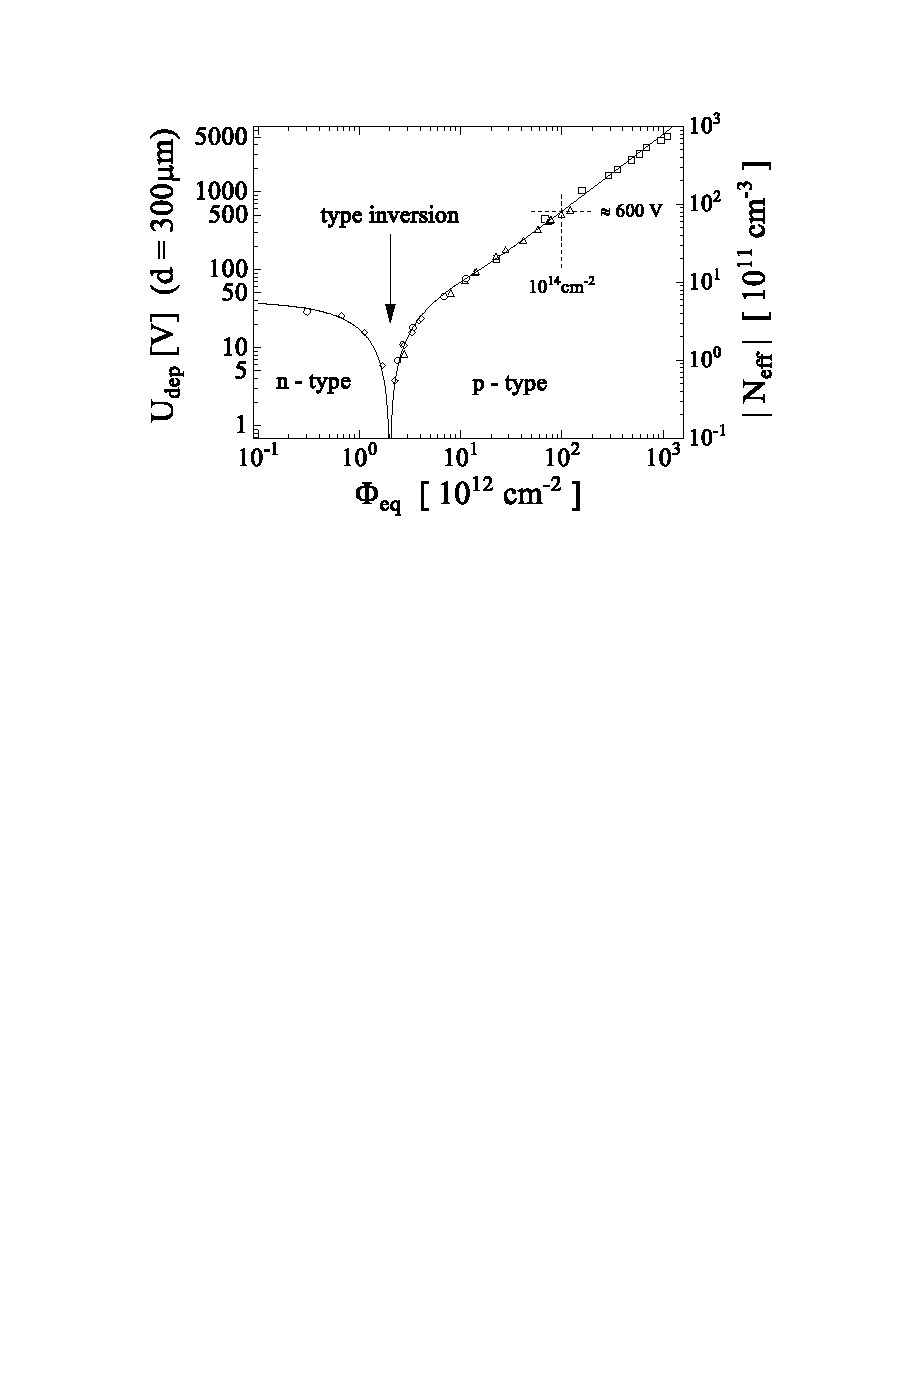
\includegraphics[width=0.5\textwidth]{typeinversion.pdf}
 \caption{\label{fig:typeinversion} Change of the full depletion voltage of a 300 $\mu$m-thick silicon 
 sensor and its absolute effective doping versus the normalized fluence, immediately after the irradiation (After~\cite{wunstors-thesis}.)}
 \end{figure}

For initial high resistivity $p-$type material the acceptor removal and donor creation effects can be 
safely neglected and the change of the effective doping concentration $N_{eff}$ has a simple linear 
dependence on the fluence $\Phi$.





\subsubsection{Annealing and Effective Doping Concentration}
%Here we will go back to a simplified scenario where  we assume a constant space charge as done 
%in the so-called ``Hamburg model''~\cite{moll-thesis}. Under this assumption we will briefly 
%describe the evolution 
%of the space charge density and the depletion voltage with time and temperature. 

 
As already mentioned in the discussion on the leakage current,  some defects can move freely 
through the crystal, they can anneal, {\it e.g.} a silicon interstitial 
could fill a vacancy in the lattice. The velocity of the annealing process depends on the average 
velocity of the movable defects, which in turn depends heavily on the temperature.
Here we give a first description of the phenomena of annealing for the space charge 
distribution in the irradiated bulk; we will come back on this topic in more detail in Chapter~\ref{chap:digi}.

With respect to the normalised rate of increase of leakage current $\alpha$, where the annealing 
is always {\it beneficial} ($\alpha$ is never increasing), the effective doping concentration $N_{eff}$
is subject to a {\it reverse} annealing too, which leads to an increase of $N_{eff}$
An example of the interplay of beneficial and reverse annealing on $N_{eff}$ is shown in 
Figure~\ref{fig:Neff_annealing}.

\begin{figure}[!htpb]
\centering
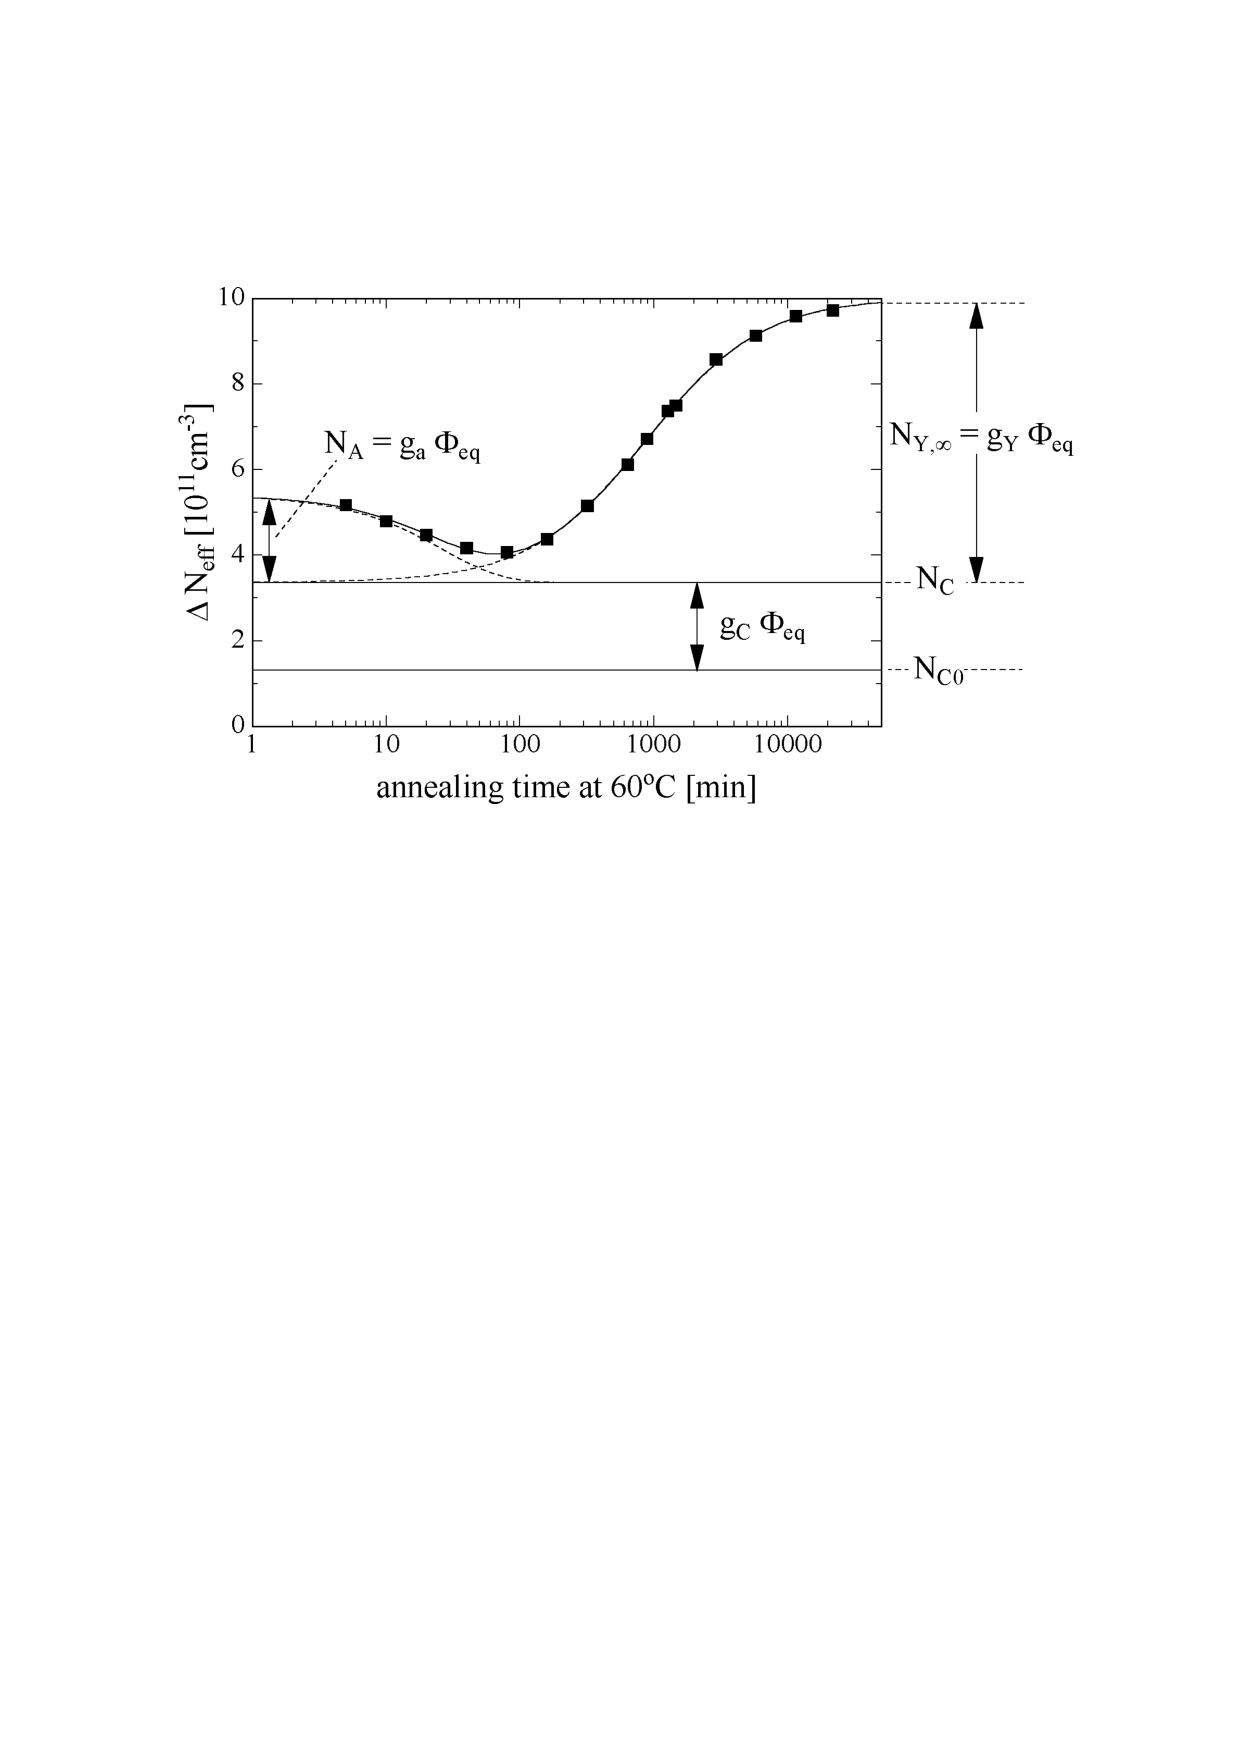
\includegraphics[width=0.5\textwidth]{Neff_annealing.pdf}
\caption{\label{fig:Neff_annealing}Annealing behaviour of the radiation induced change in effective 
doping concentration $\Delta N_{eff}$ at 60$^{\circ}$C. The shown example is a $n-$type high 
resistivity sample, neutron-irradiated with a fluence of 1.4$\times$10$^{13}$. 
(After~\cite{moll-thesis})}
\end{figure}


For the effective doping or the bias voltage respectively the annealing process is subdivided into 
two periods. 
The beneficial annealing period which extends roughly for the first 80 minutes at 60$^{\circ}$C; 
after the beneficial annealing period the effective doping concentration, hence the depletion voltage 
$V_{depl}$, is  reduced to a minimum. Afterwards, the reverse annealing process sets in and leads 
to an increase 
of the $V_{depl}$, exceeding the initial $V_{depl}$ directly after 
irradiation.

\subsubsection{Heavily Irradiated Silicon Detectors}

In the studies presented in the previous Sections the determination of the fluence and time 
dependence of the effective doping concentration  $N_{eff}$
simple unstructured diodes were used~\cite{moll-thesis} 
and the full depletion voltage was deduced from CV 
measurements (Eq.~\ref{eq:CV}). This method assumes a constant space charge which is not 
given 
for highly irradiated sensors where the field shows a double peak~\cite{Li1992}. This can be 
qualitatively explained by defects being filled by carriers drifting under reverse bias voltage. 
In a $n-on-n$ detector electrons will flow toward the $n^+$ electrode while holes toward the $p^+$ one. 
So the chances of having a negatively charged defect close to the   $n^+$ electrode  are higher 
than a positively charged one; the opposite goes for the defects close to the $p^+$ electrode. 
The mechanism was first proposed in~\cite{bib:DP};
 it is illustrated in Figure~\ref{fig:Chiochia2005DP}.
\begin{figure}[htpb]
 \centering
 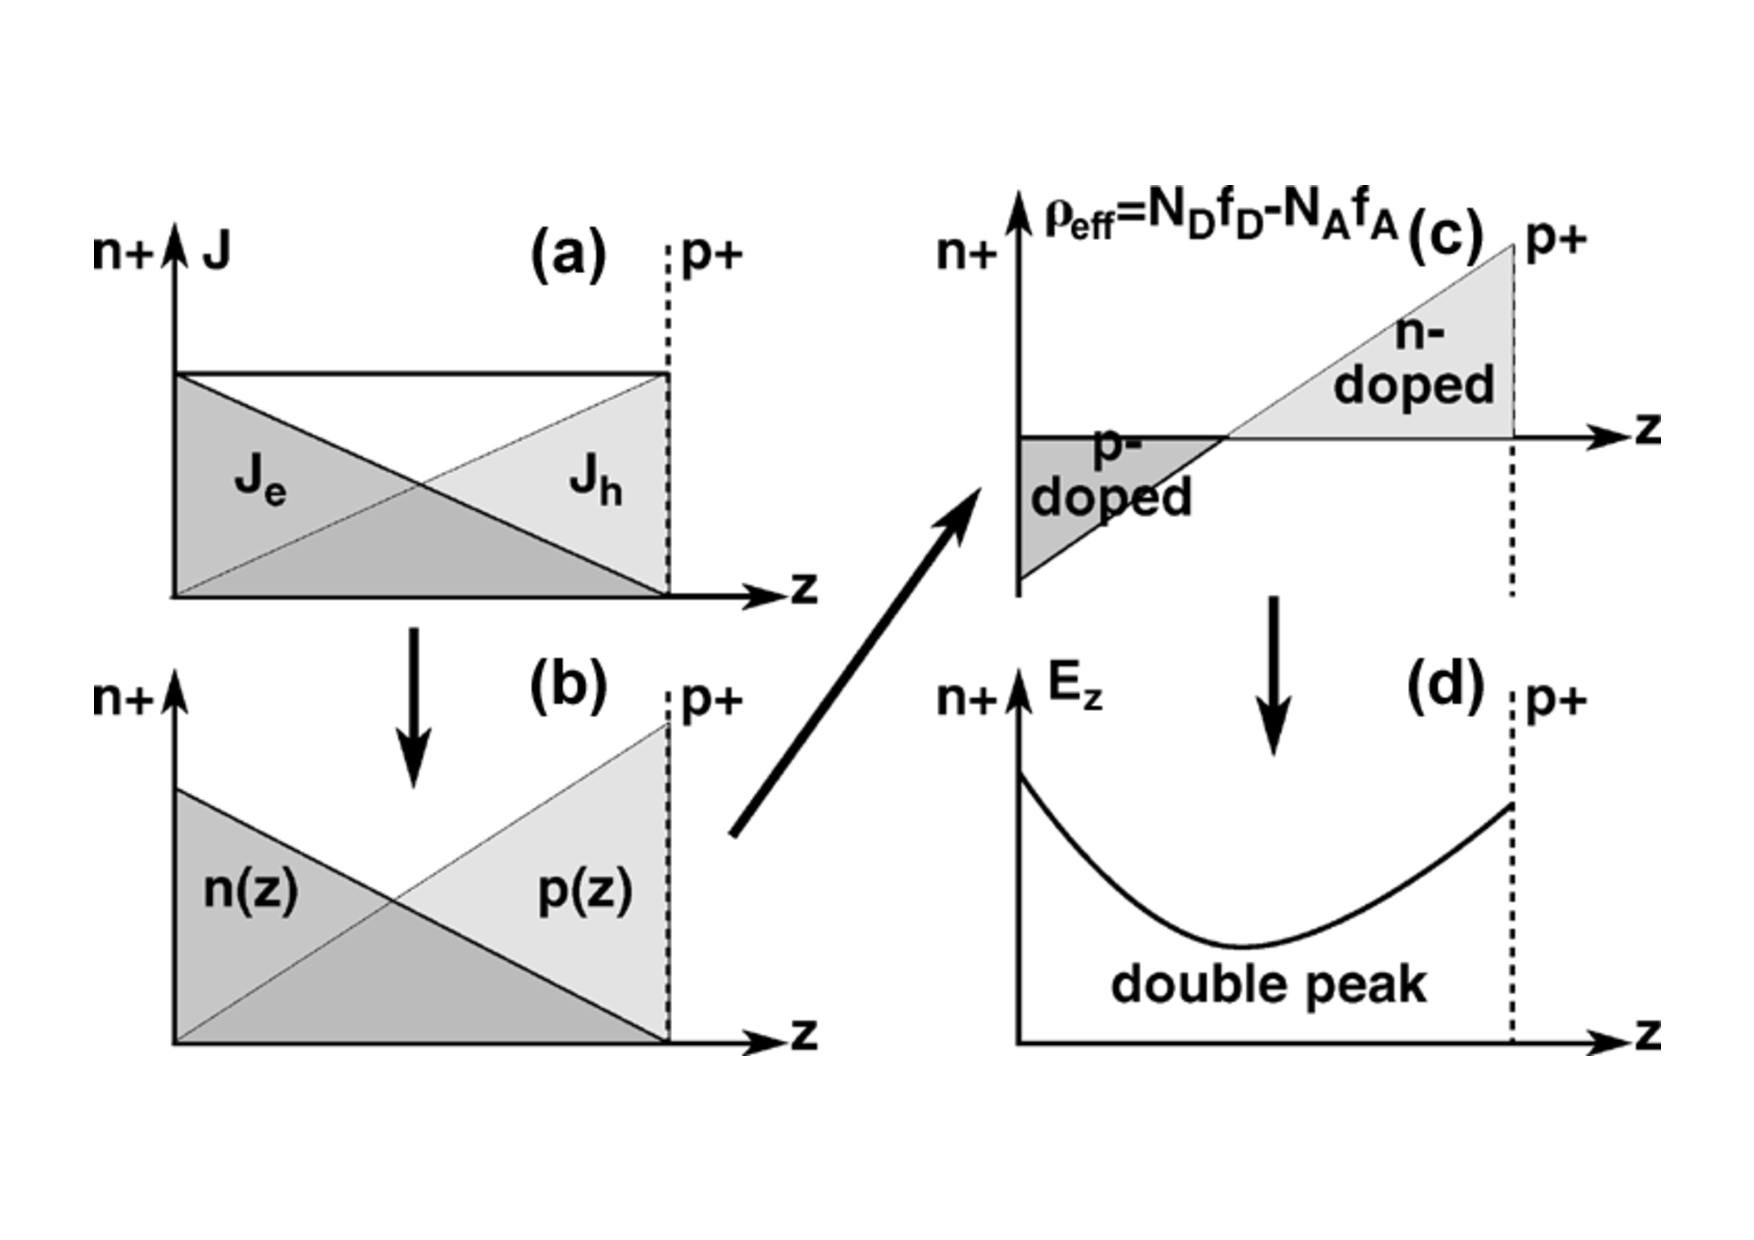
\includegraphics[width=0.5\textwidth]{Chiochia2005DP.pdf}
 \caption{\label{fig:Chiochia2005DP} An illustrative sketch of the explanation of the double peak effect in electric field  for a reverse biased irradiated device. (After~\cite{Chiochia2005})}
 \end{figure}

In case of double peak in the electric field distribution the numbers derived for depletion voltage and 
effective doping concentration form the CV measurements 
are effective or average numbers.

An example of a $C^{-2}$V measurement for an irradiated device is shown in Figure~\ref{fig:irrCV}.
\begin{figure}[htpb]
 \centering
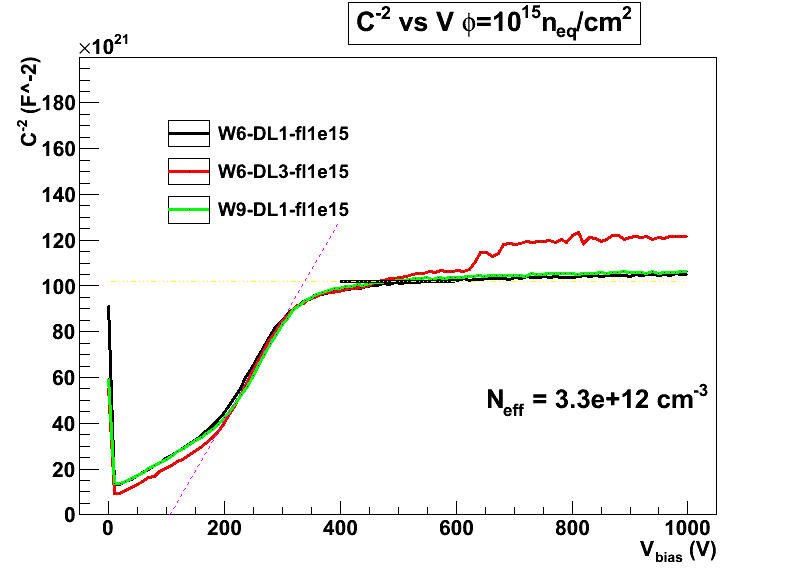
\includegraphics[width=0.5\textwidth]{irrad2011-fl1e15-best.png}
 \caption{\label{fig:irrCV} $C^{-2}$~vs~V of a 285~$\mu$m thick $n-on-p$ diode irradiated at CERN 
 with 24~GeV/c protons, with an integrated fluence of $\Phi=1\times10^{15}$~n$_{\rm eq}$/cm$^2$, 
 after having being annealed for 80 minutes at 60$^\circ$C. Results from three diodes, 
 coming from 2 different 
 wafers, and with different number of GRs are reported.}  
 \end{figure}
 
 The $C^{-2}$ vs V curves reported in Figure~\ref{fig:irrCV}, whose slope is proportional to the 
 effective doping concentration $N_{eff}$in un-irradiated material, show a change in slope around 
 200~V; the curves reach a pleateau around 300~V. These two slopes are connected with the 
 electric field setting on from both the front and the back side of the detector.


\subsection{Trapping}
\label{sec:trapping}
Radiation-induced defects are responsible not only for generation-recombination centers increasing 
the leakage current and charged defects with dramatic influence on the full depletion voltage but 
also for trapping centers. Traps are mostly unoccupied in the depletion region due to the lack of free 
charge carriers and can hold or trap part of the signal charge for a time longer than the charge 
collection time and so reduce the signal amplitude. 

The typical trapping time $\tau_{tr}$ gets shorter and shorter with larger and larger fluence $\Phi$; it 
has 
been found it is proportional to the inverse of fluence:

\begin{equation}
\tau_{tr}^{-1}=\beta\Phi
\label{eq:trappingtime}
\end{equation}

Measured values for $\beta$ are about $4-6\times10^{-16}$~cm$^2$/ns for electrons 
and $6-8\times10^{-16}$~cm$^2$/ns for holes~\cite{KRAMBERGER2002297}. Larger $\beta$ 
values for holes than for electrons mean that trapping is most severe for the former than the latter. 
It has also to be noticed that the hole mobility is about 1/3 of the electron one; so holes move 
slower and gets trapped more. Given these two conditions nowadays electrons collecting 
silicon detectors, like $n-on-n$ and $n-on-p$, are favoured over holes collecting ones, like
 $p-on-n$.  

Given that in the saturation regime carriers take about 1~ns to traverse 100~$\mu$m in Silicon, 
the trapping effect starts to be the most impacting radiation damage effect after fluences in excess of $
\Phi=1\times10^{15}$~n$_{\rm eq}$/cm$^2$. In Appendix~\ref{sec:CCEirr} some estimations 
for the expected charge collection efficiency (CCE) in irradiated silicon pads are presented. 
For example, after  $\Phi=1\times10^{16}$~n$_{\rm eq}$/cm$^2$ a 100~$\mu$m thick pad diode 
will be able to collect only about 27\% of the signal amplitude prior to irradiation.

After irradiation segmented detectors, like DSSDs and HPDs, will allow to achieve CCE higher than 
the one for pads thanks to the steeper slope of the Ramo potential close to the collecting electrode; 
this will be treated in Chapter~\ref{chap:digi}.

Trapping time $\tau_{tr}$ evolves with time and temperature as leakage current and depletion voltage 
do. In~\cite{KRAMBERGER2007762} it is shown that the trapping asymptotic probabilities  of
holes (electrons) will be around 30\% larger (15\% smaller)
than initial probabilities at the same total fluence.

\section{Summary}
\label{sec:SiliconSummary}

In this Chapter we reviewed the basics of semiconductor physics and the reasons for the 
success of silicon tracking sensors for HEP experiments. Advantages and limitations of the 
different silicon detectors were discussed. In the end radiation damage, one of the biggest challenges for 
actual and future silicon detectors at hadron colliders, was presented.
This introduction will serve as a base for the next chapters.


   
